%%____________________________________________________________________________||
\section{Characterisation of the signal and control regions}
\label{sec:yields}

%%____________________________________________________________________________||
\subsection{Distributions for key analysis variables \label{sec:mc-data-comp}}

The hadronic signal region selection and control regions are detailed in Sec.~\ref{sec:selection}. The relevant data/MC plots are presented here, corresponding to symmetric, asymmetric and monojet selection. The distributions help to understand the MC modeling of key variables. The MC distributions are normalised to their corresponding luminosities in Run 2015D. These luminosities are calculated  with the consideration of the HLT triggers used in each region. The data/MC scale factors are shown in all figures.

%%____________________________________________________________________________||
\begin{figure}
    \begin{center}
        \subfigure {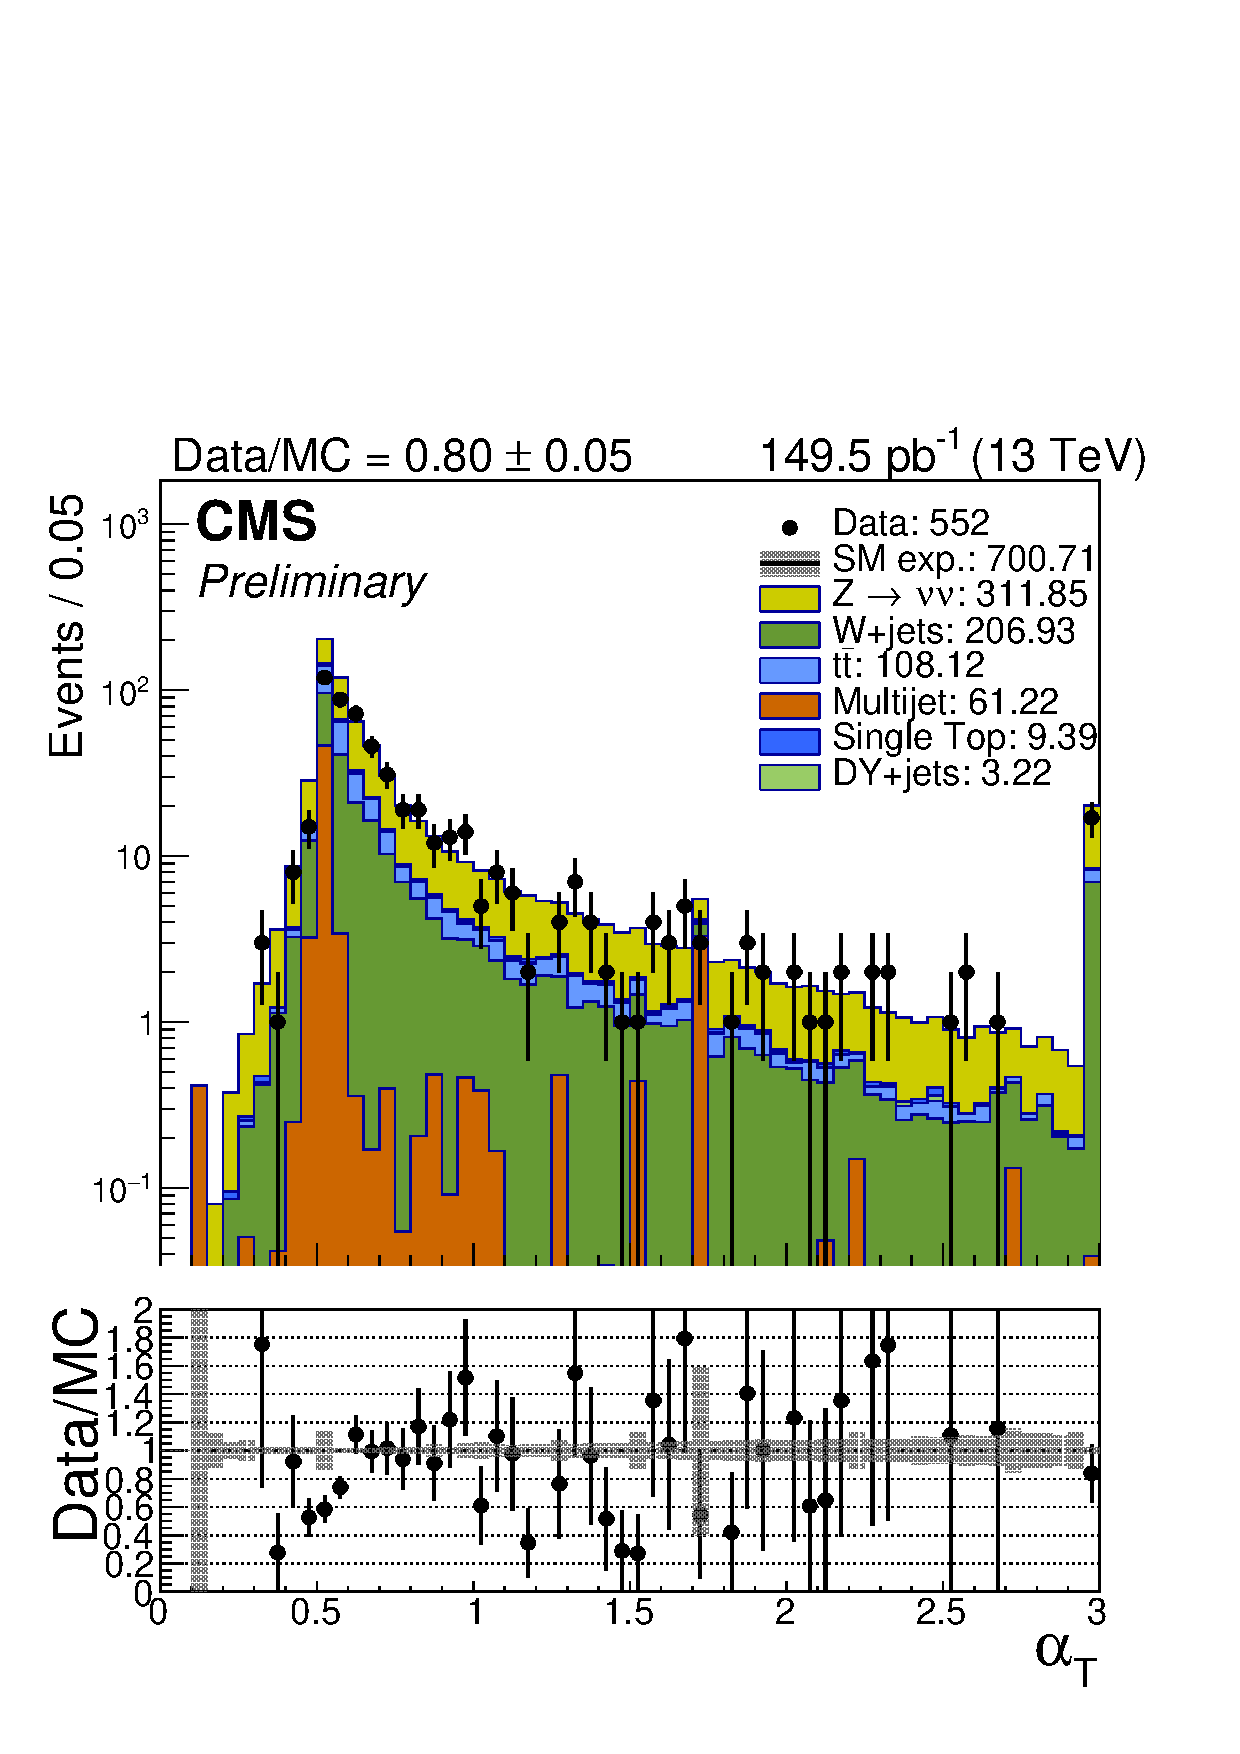
\includegraphics[width=0.5\textwidth]{figures/distributions/Signal/alphaT_sym.pdf}} ~~
        \subfigure {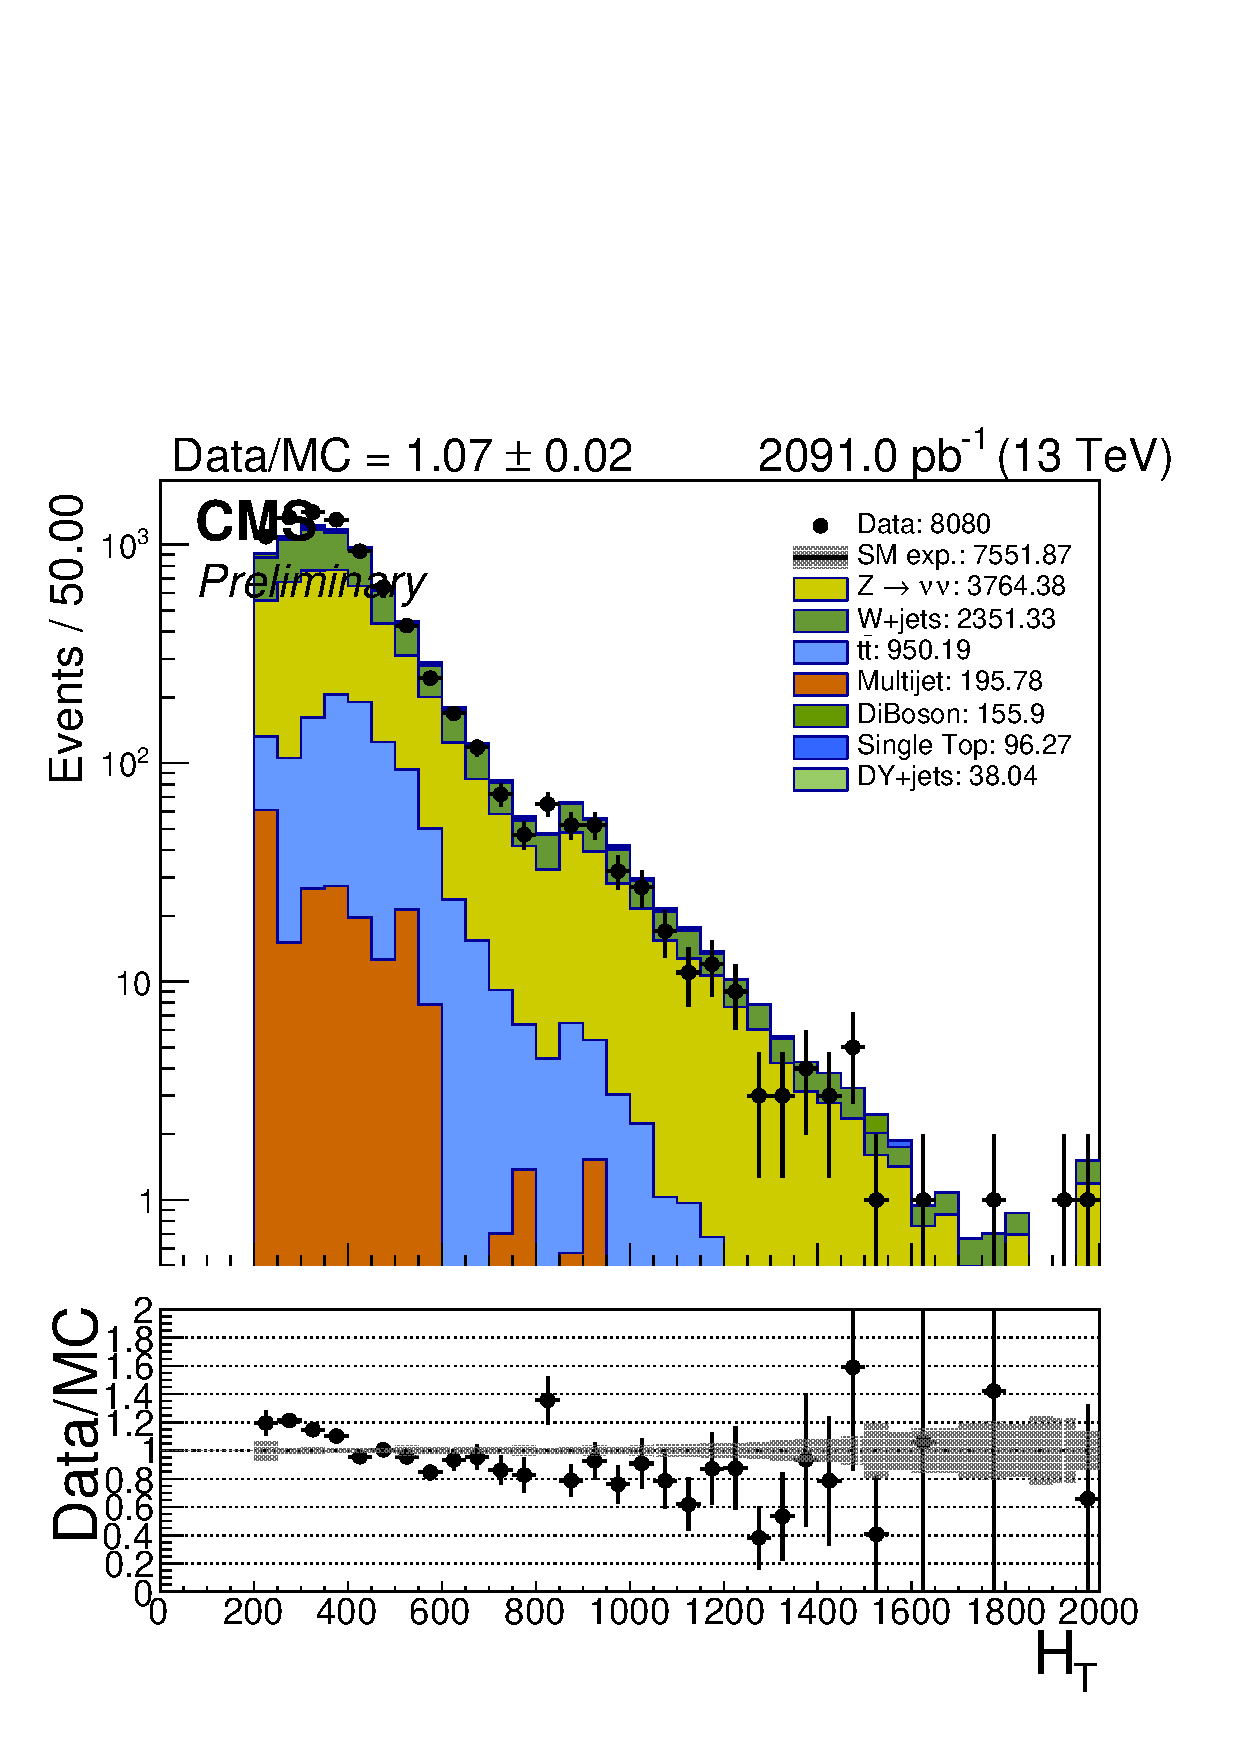
\includegraphics[width=0.5\textwidth]{figures/distributions/Signal/ht40_sym.pdf}} \\
        \subfigure {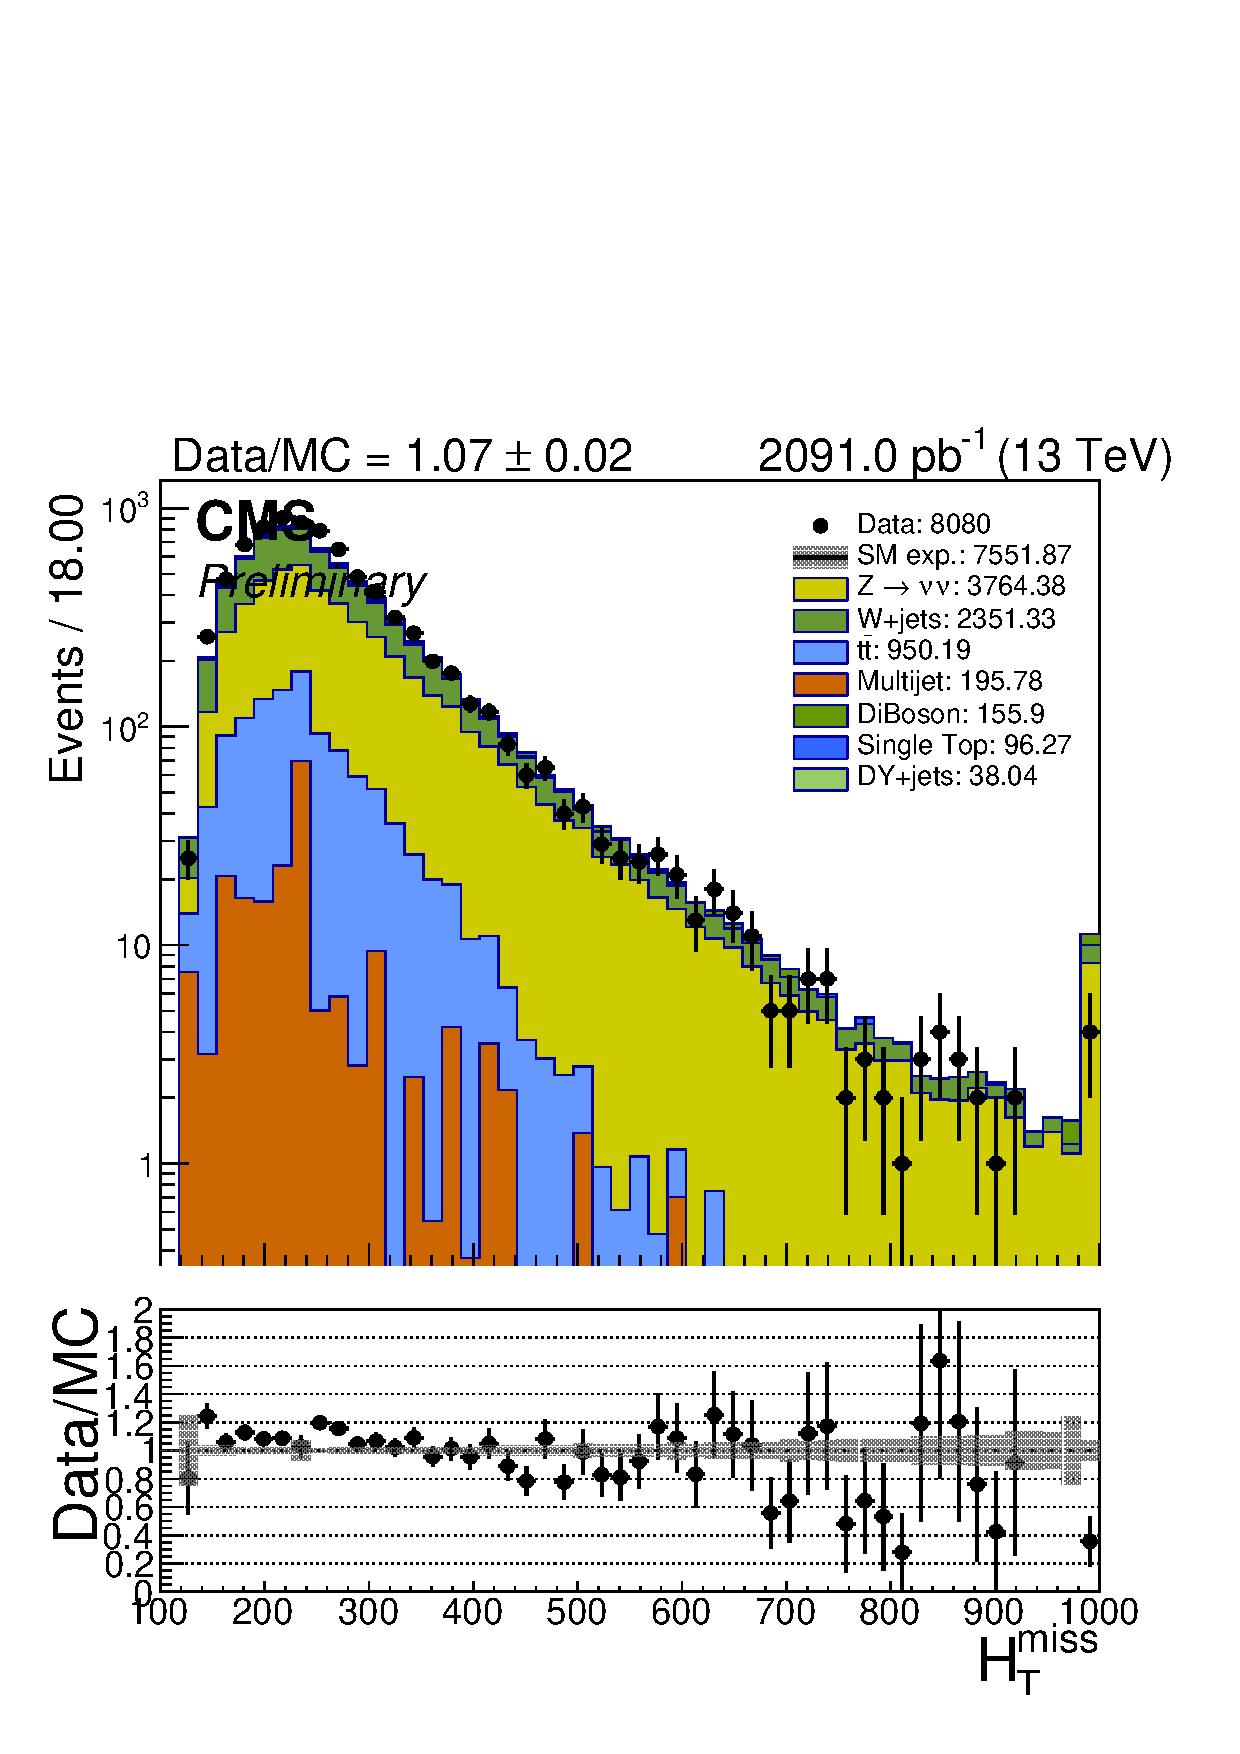
\includegraphics[width=0.5\textwidth]{figures/distributions/Signal/mht40_pt_sym.pdf}} ~~
        \subfigure {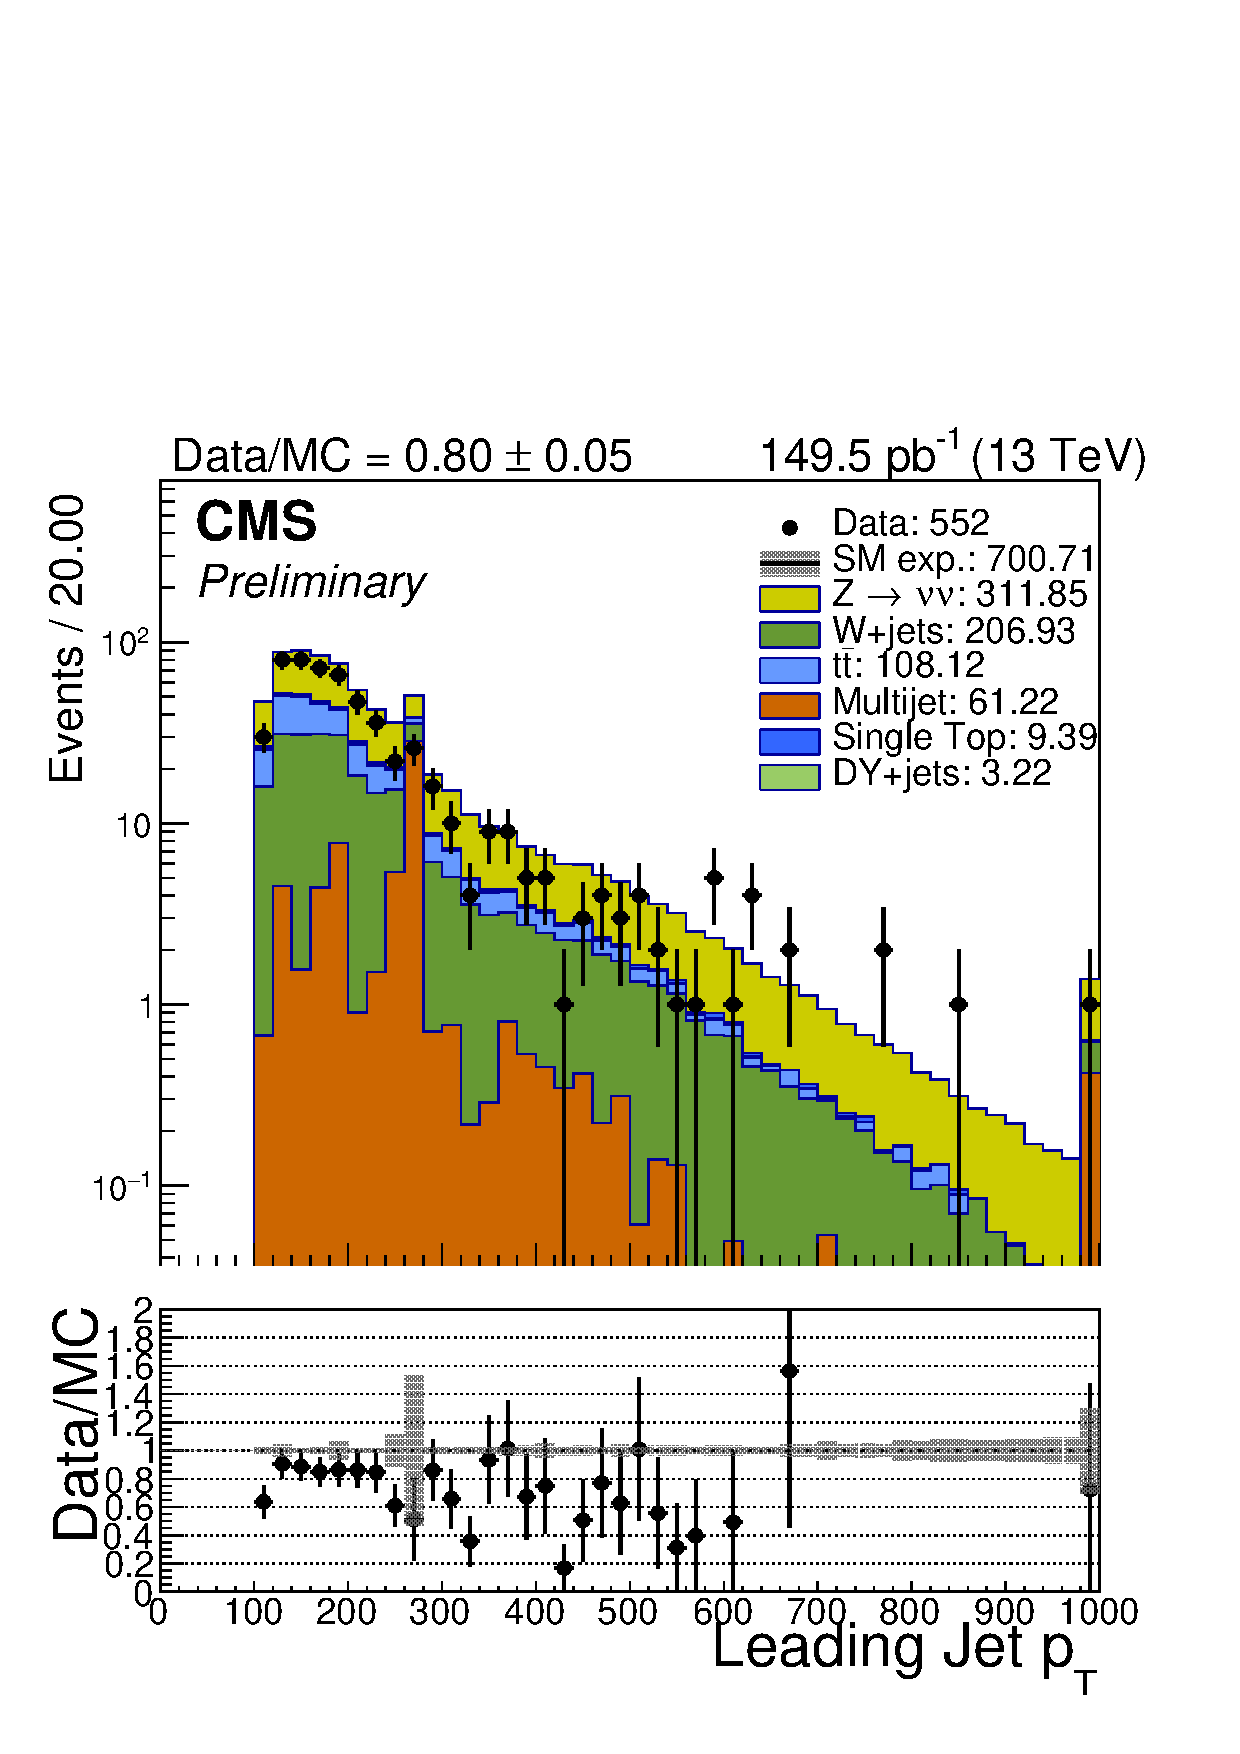
\includegraphics[width=0.5\textwidth]{figures/distributions/Signal/jet_pt[0]_sym.pdf}} \\
        \caption{Key analysis variables for hadronic signal region (symmetric bins)}
        \label{fig:distribution_signal_sym}
    \end{center}
\end{figure}

\begin{figure}
    \begin{center}
        \subfigure {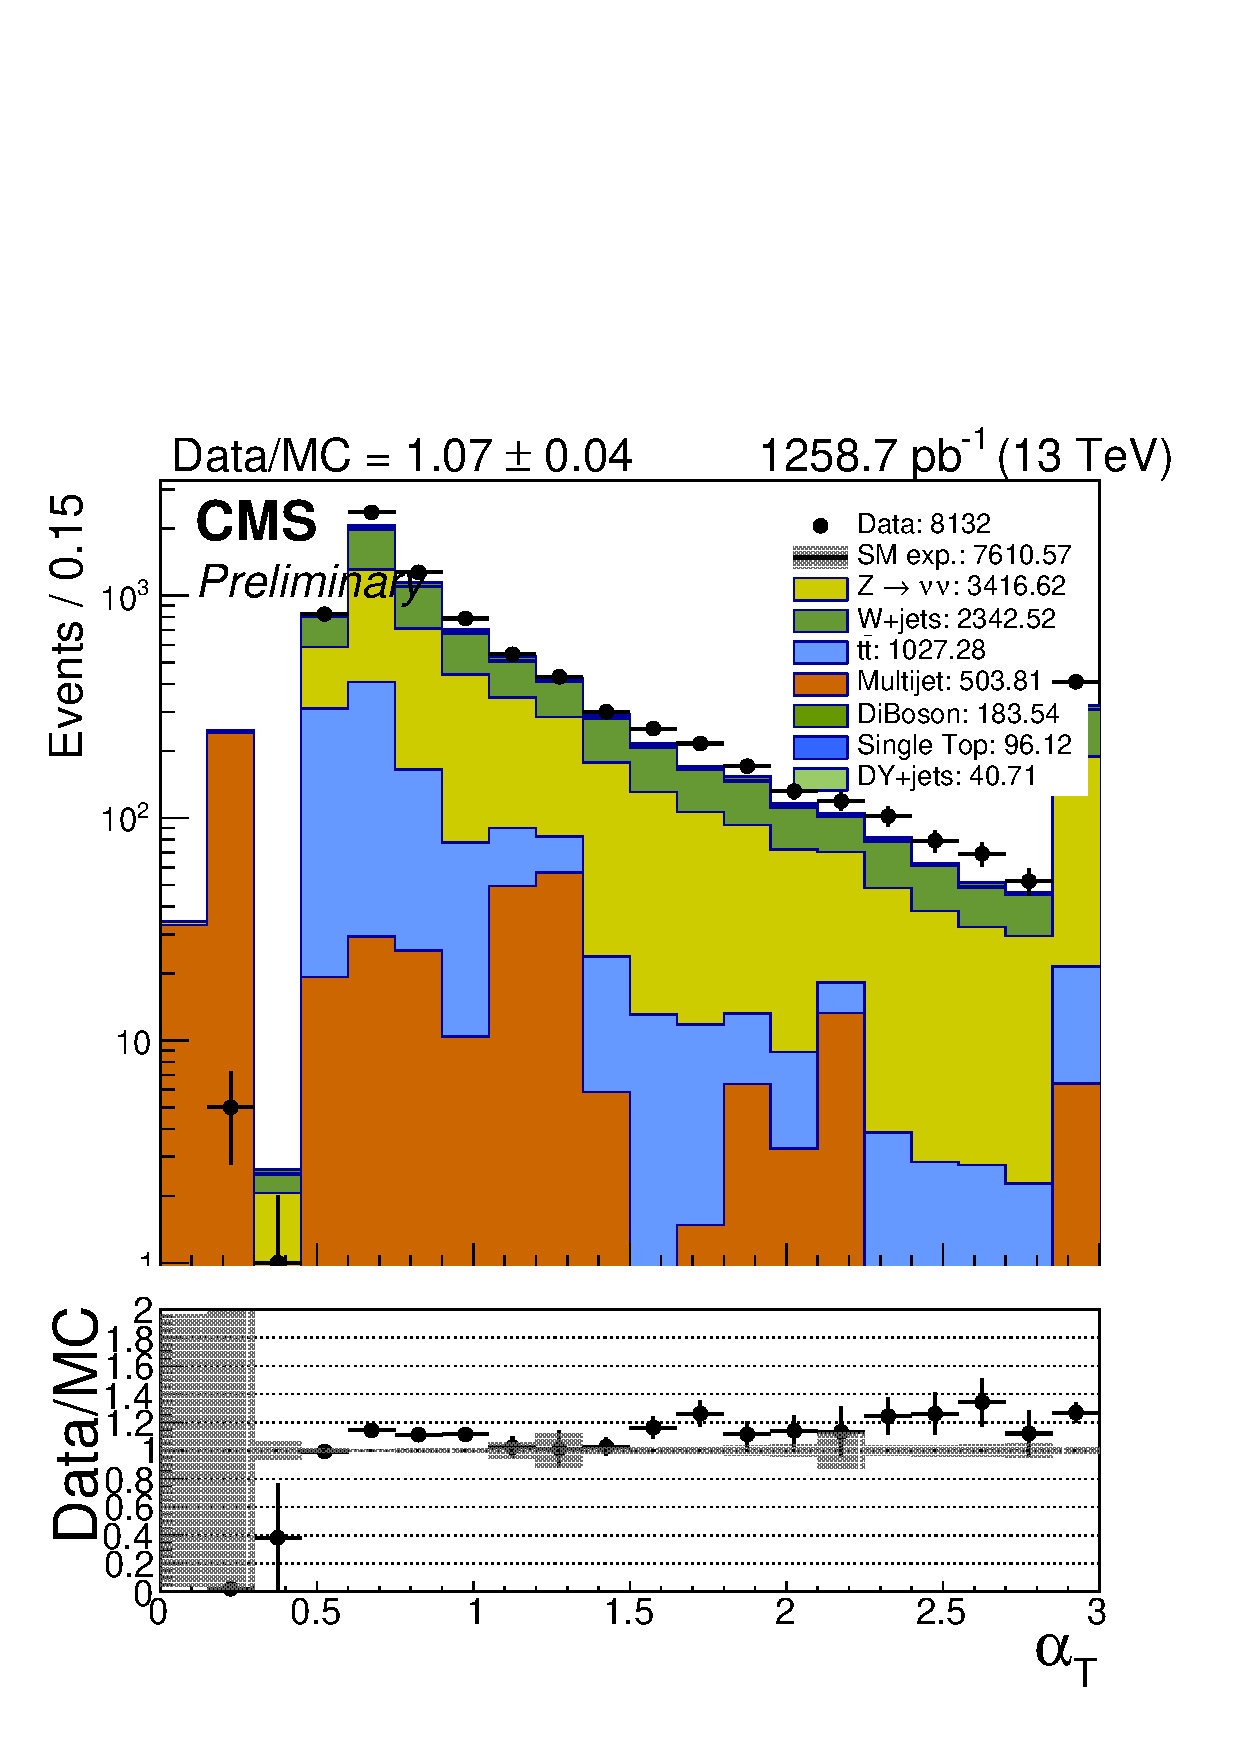
\includegraphics[width=0.5\textwidth]{figures/distributions/Signal/alphaT_asym.pdf}} ~~
        \subfigure {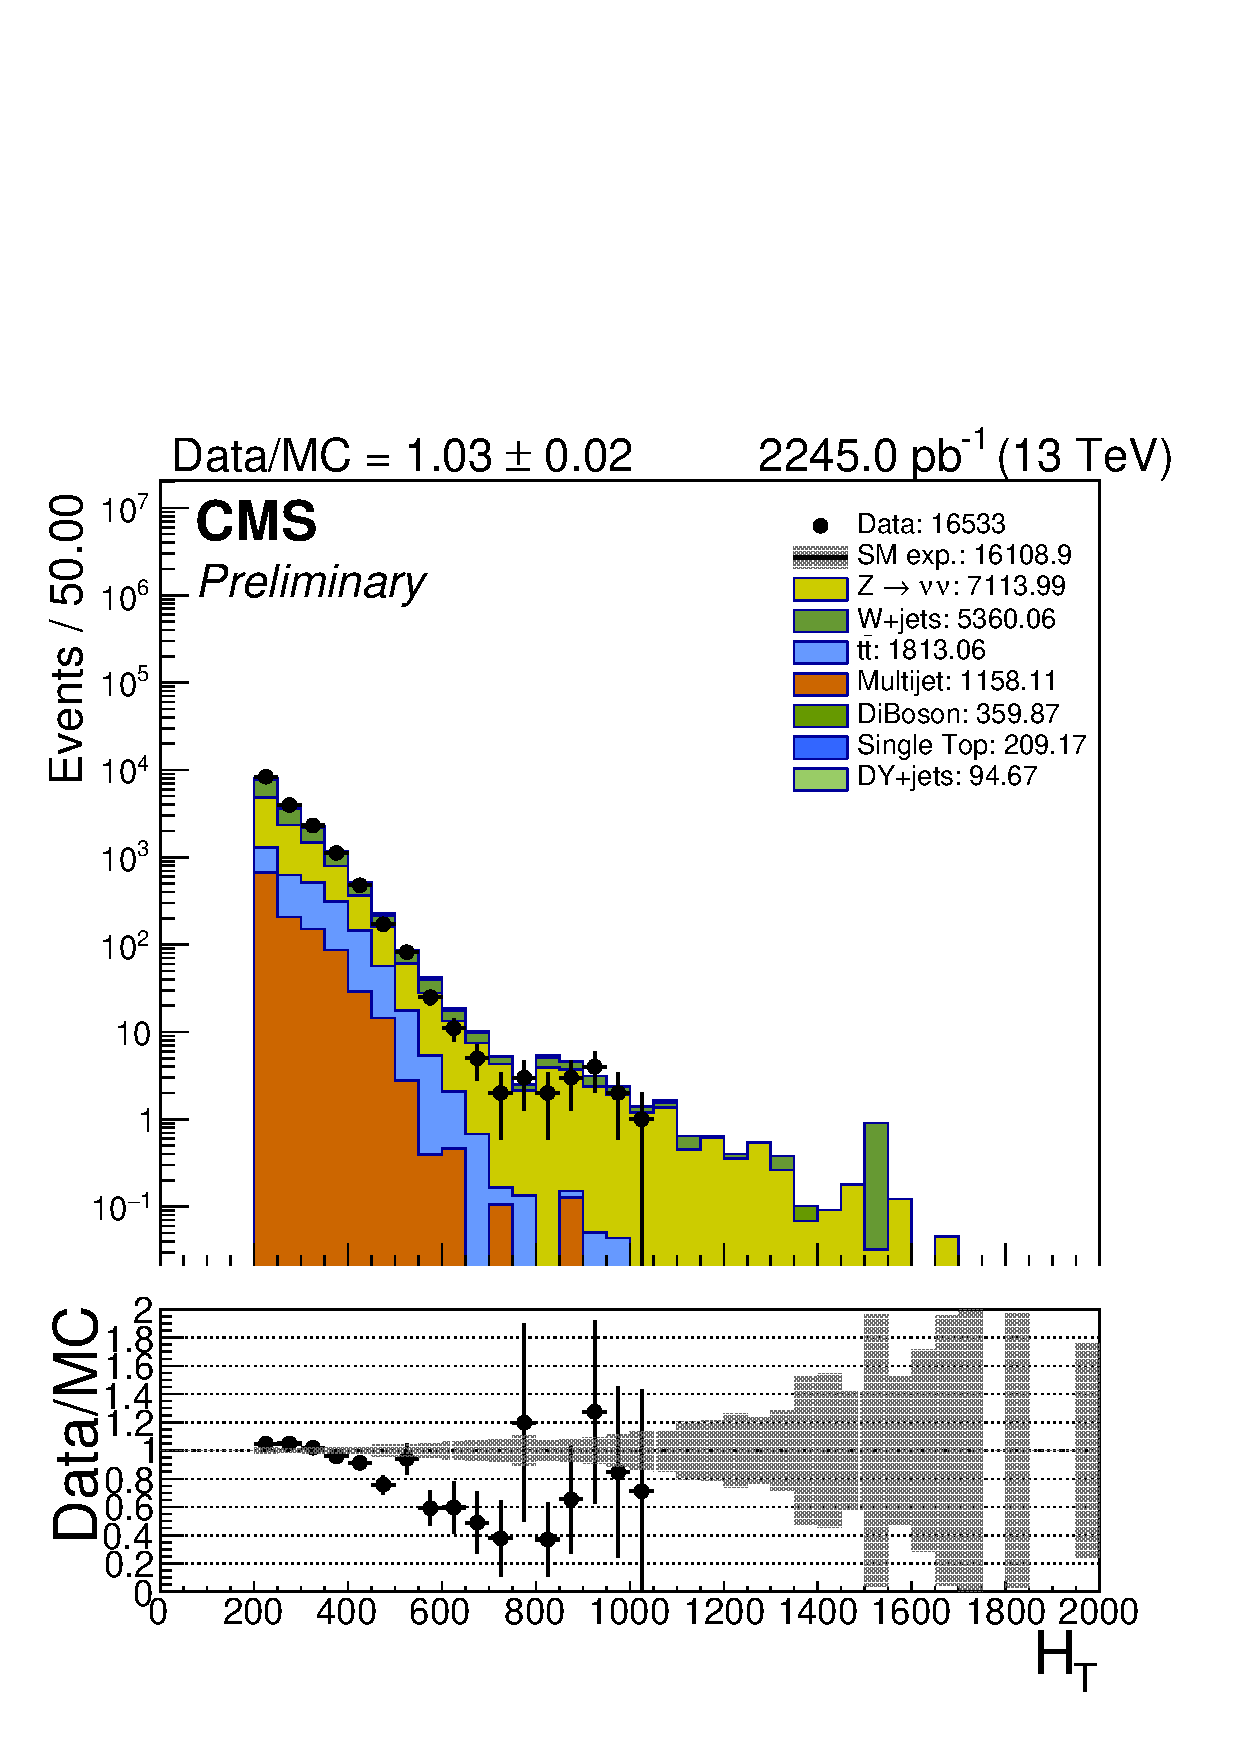
\includegraphics[width=0.5\textwidth]{figures/distributions/Signal/ht40_asym.pdf}} \\
        \subfigure {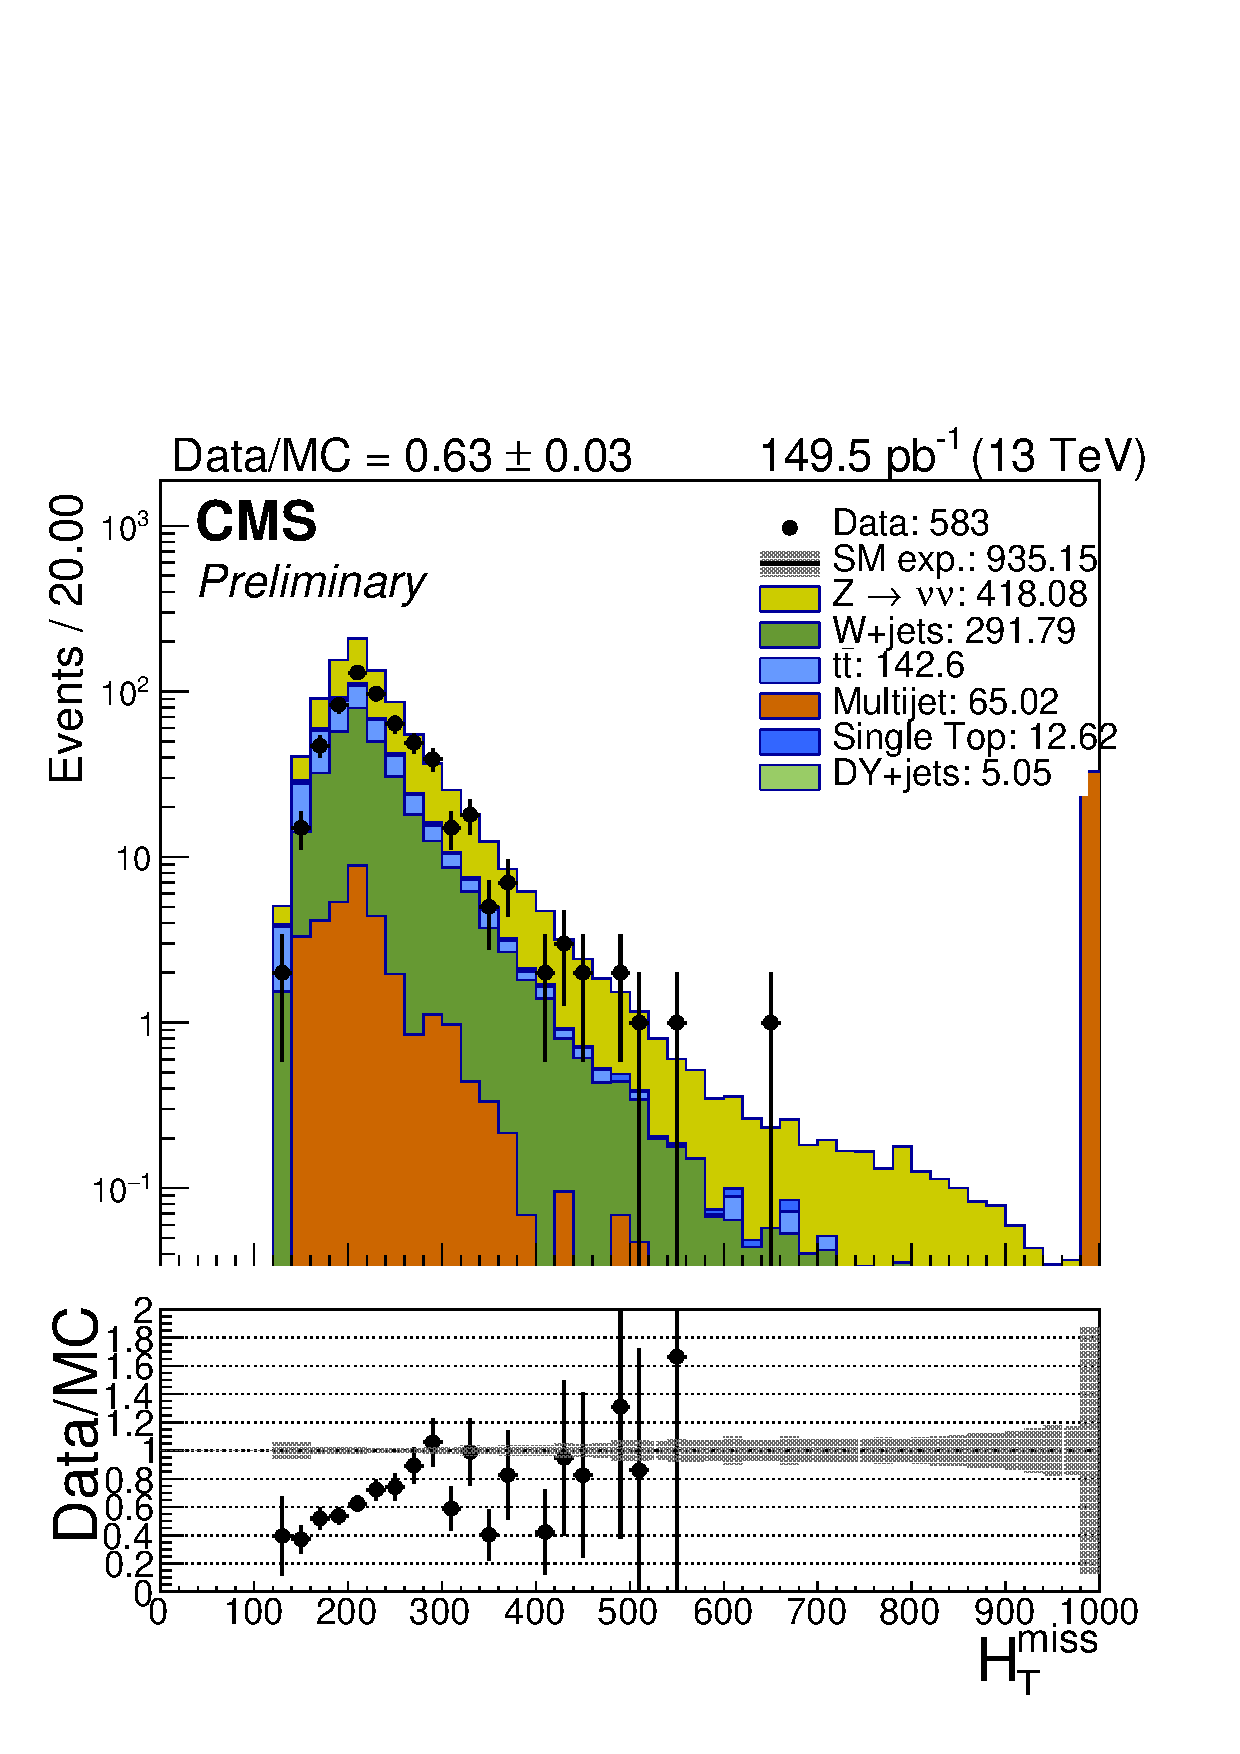
\includegraphics[width=0.5\textwidth]{figures/distributions/Signal/mht40_pt_asym.pdf}} ~~
        \subfigure {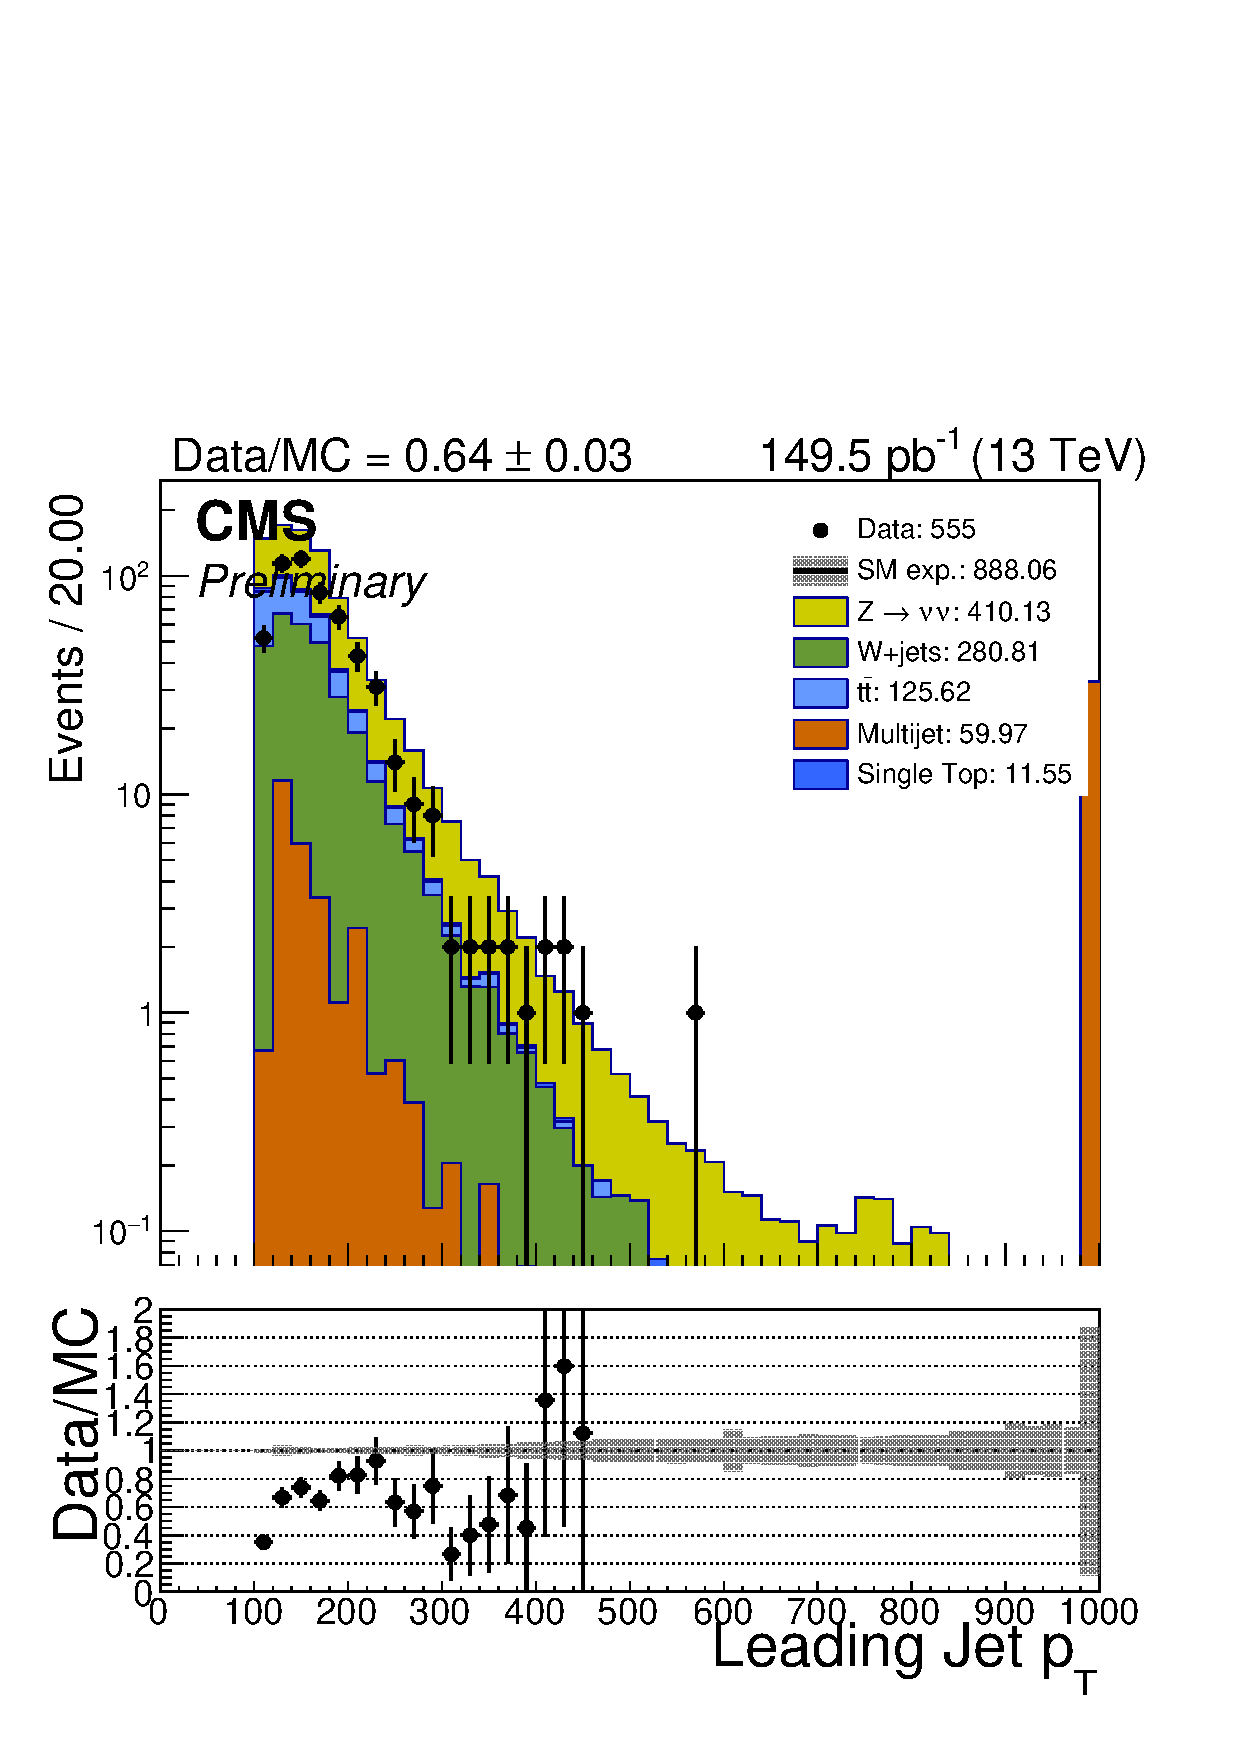
\includegraphics[width=0.5\textwidth]{figures/distributions/Signal/jet_pt[0]_asym.pdf}} \\
        \caption{Key analysis variables for hadronic signal region (asymmetric bins)}
        \label{fig:distribution_signal_asym}
    \end{center}
\end{figure}

\begin{figure}
    \begin{center}
        \subfigure {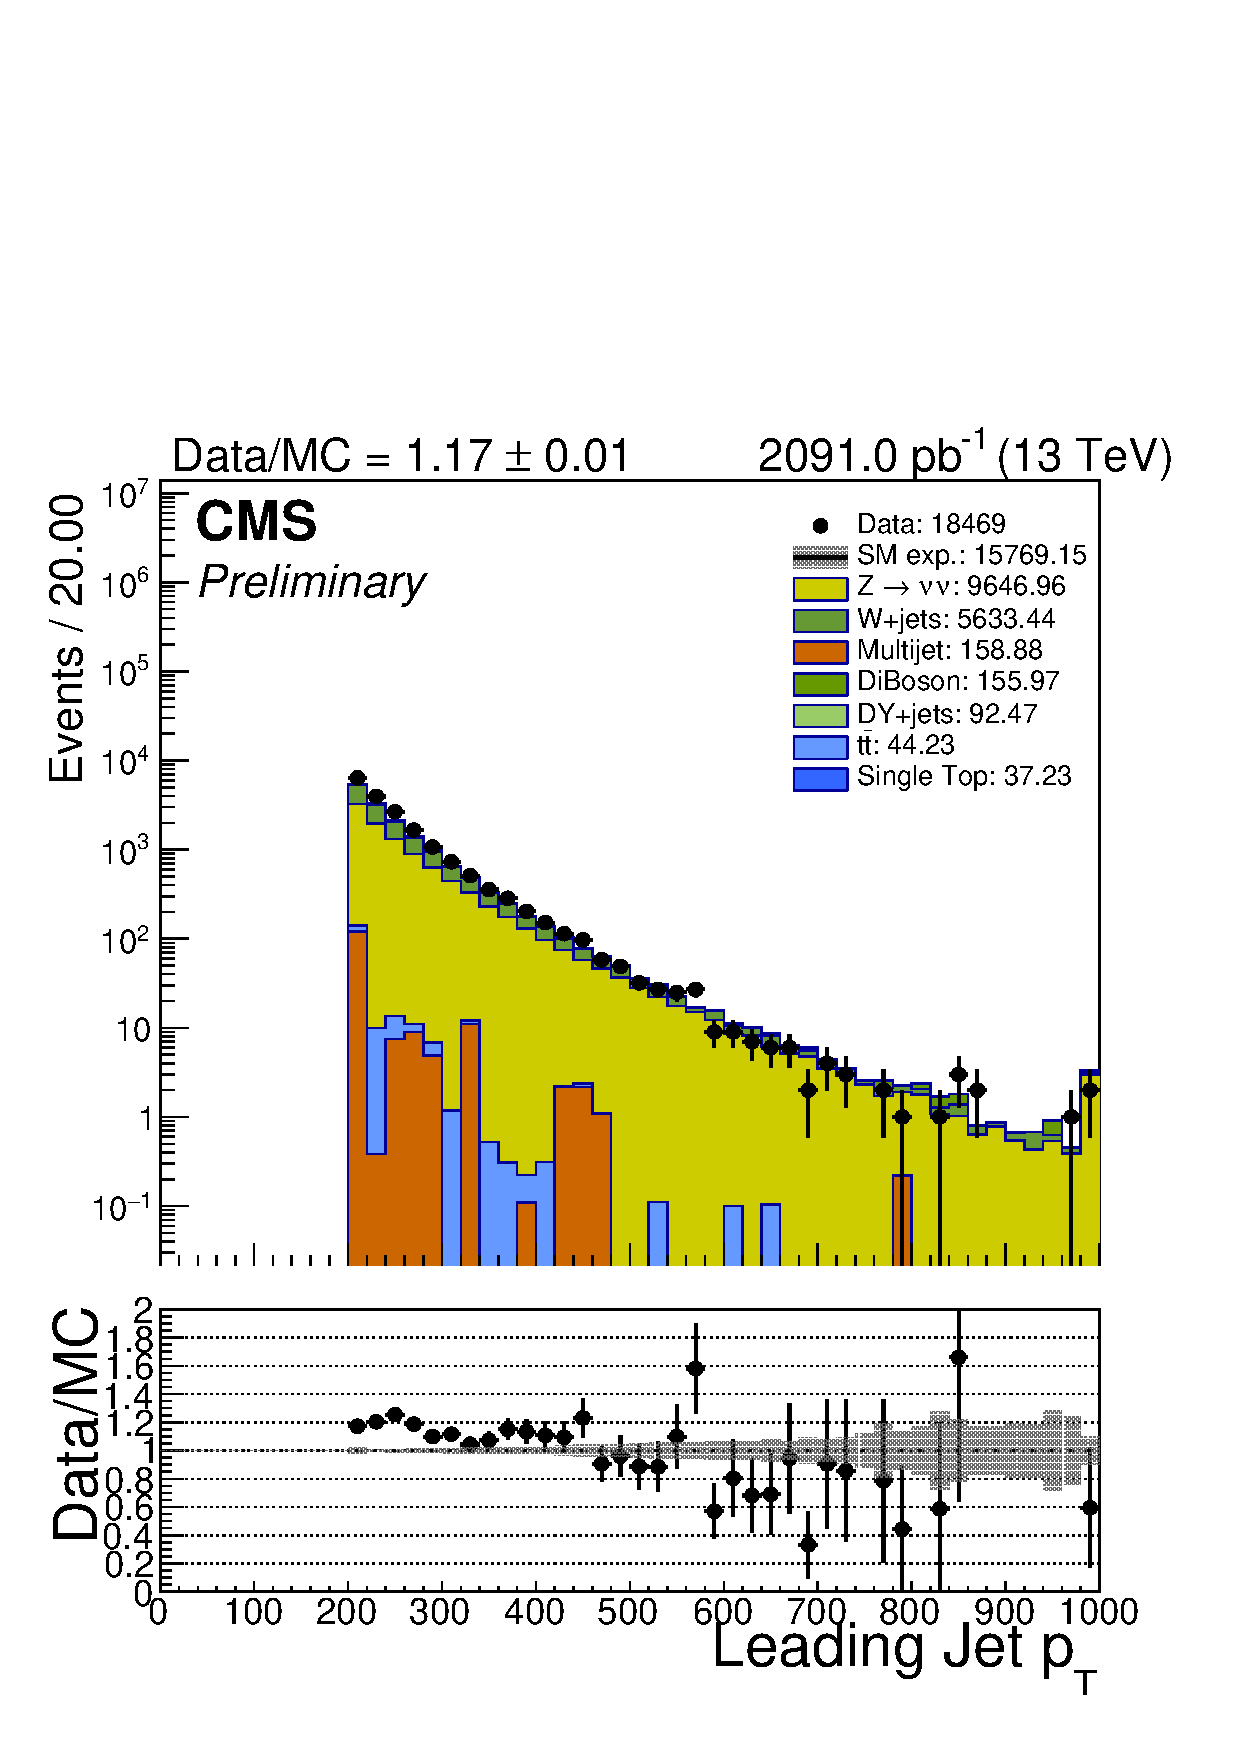
\includegraphics[width=0.5\textwidth]{figures/distributions/Signal/jet_pt[0]_eq1j.pdf}} ~~
        \subfigure {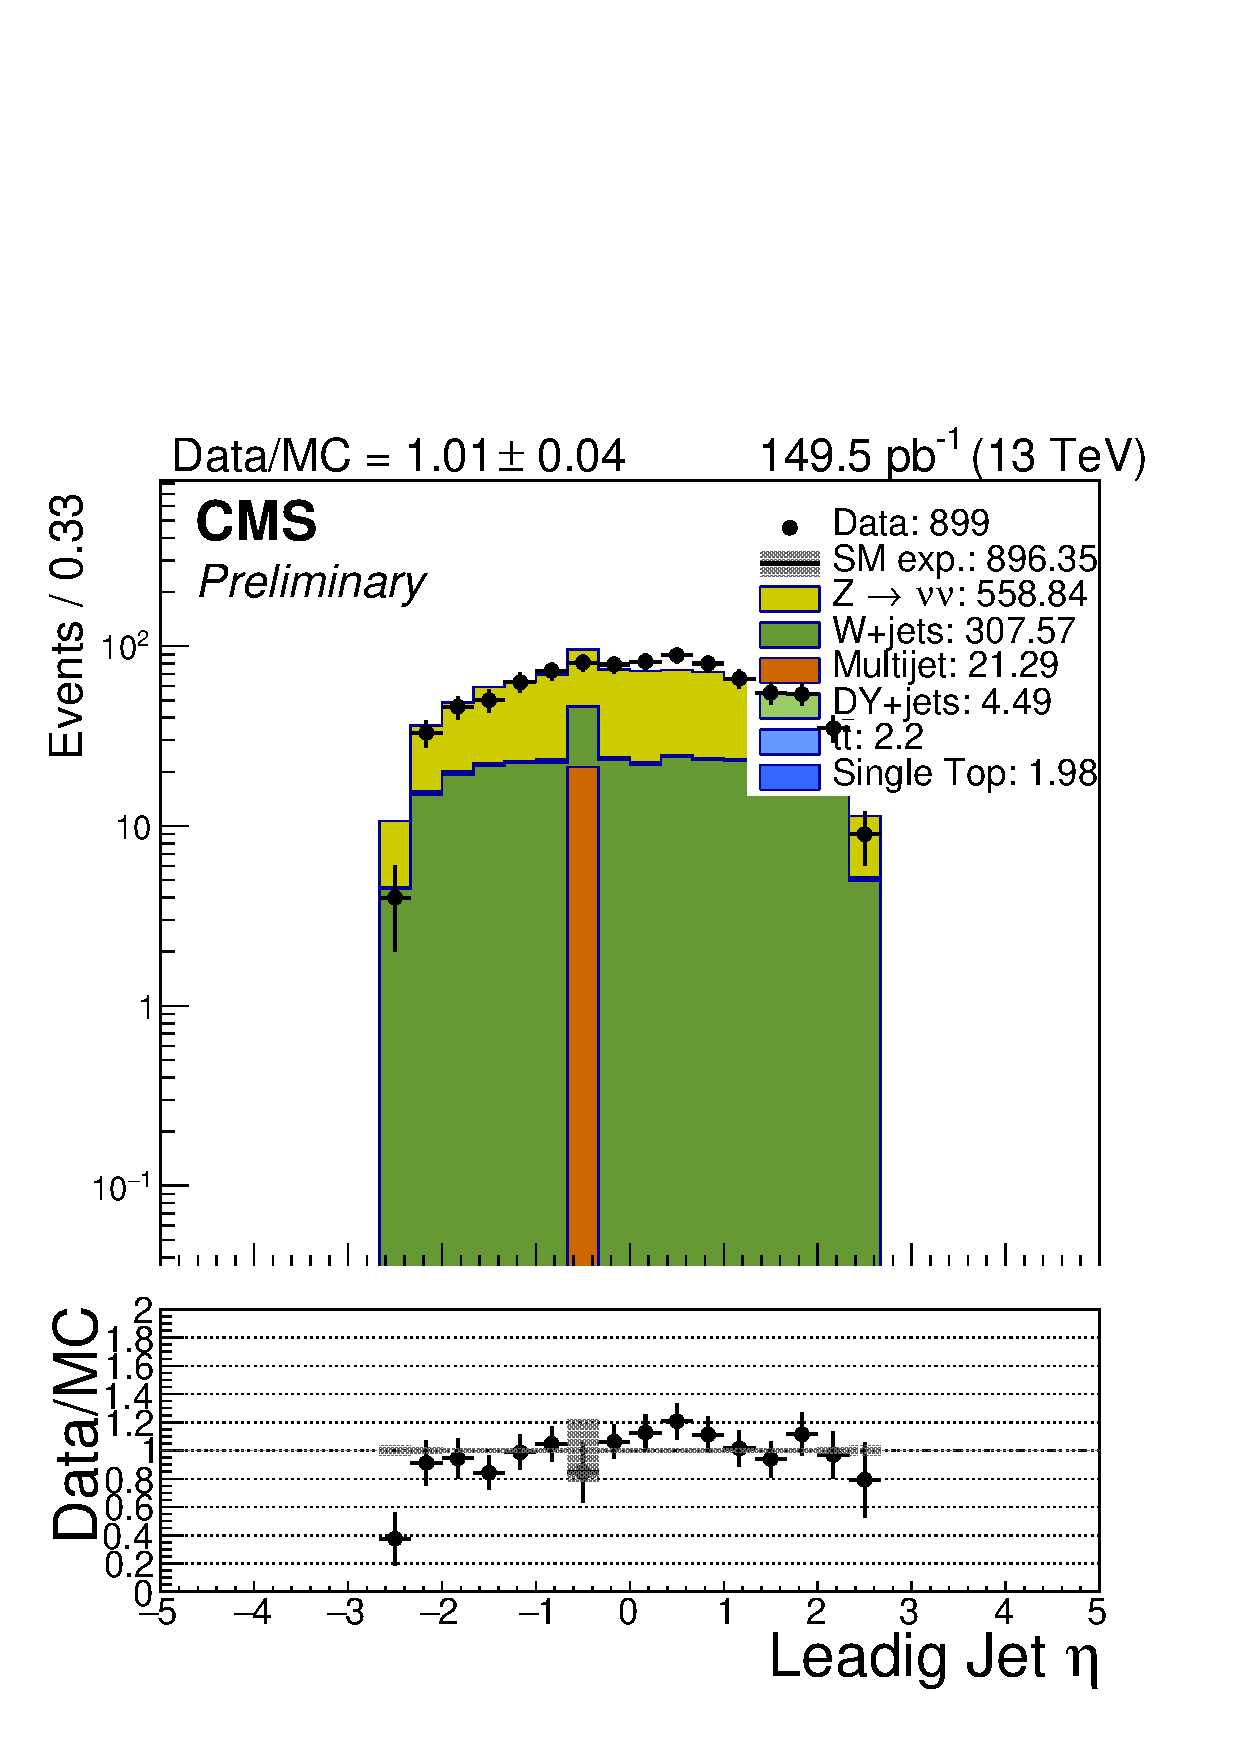
\includegraphics[width=0.5\textwidth]{figures/distributions/Signal/jet_eta[0]_eq1j.pdf}} \\
        \subfigure {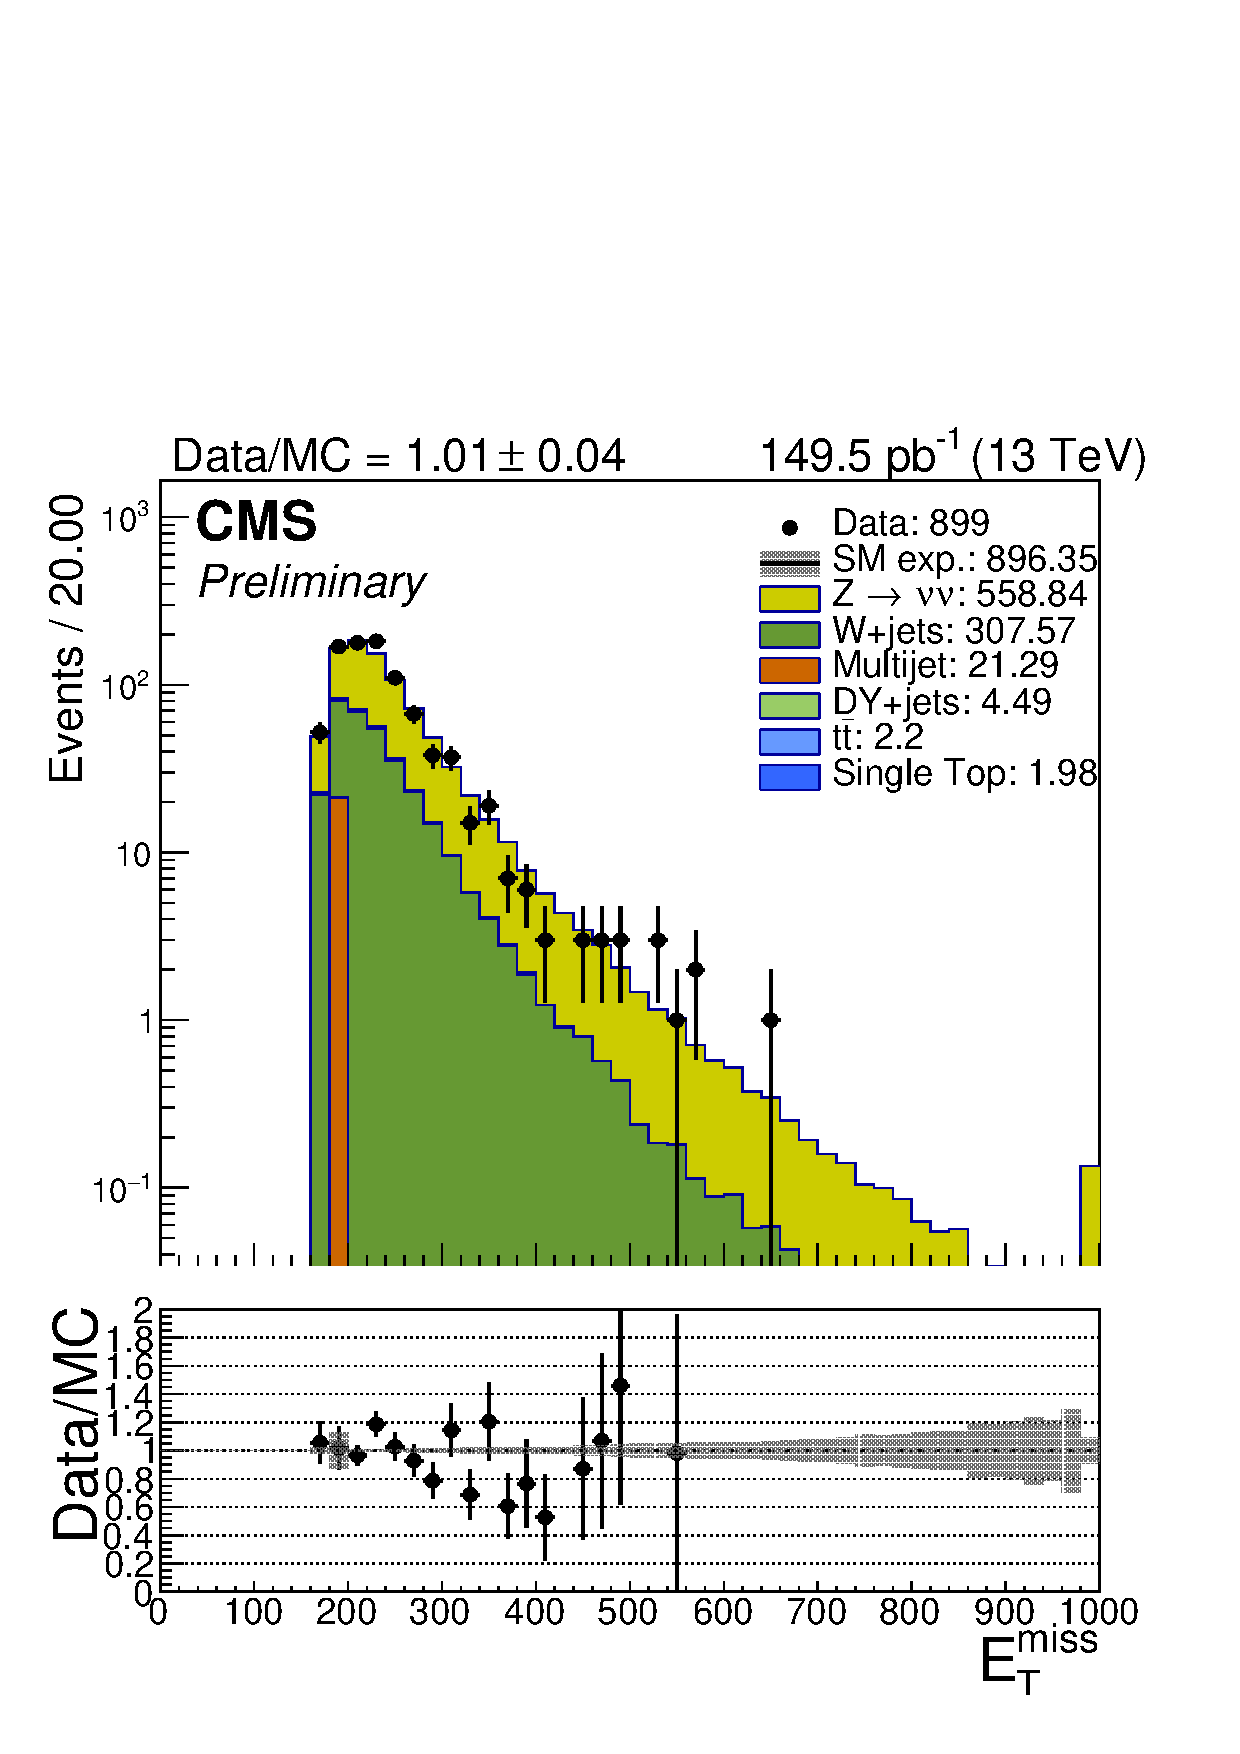
\includegraphics[width=0.5\textwidth]{figures/distributions/Signal/met_pt_eq1j.pdf}} ~~
        \subfigure {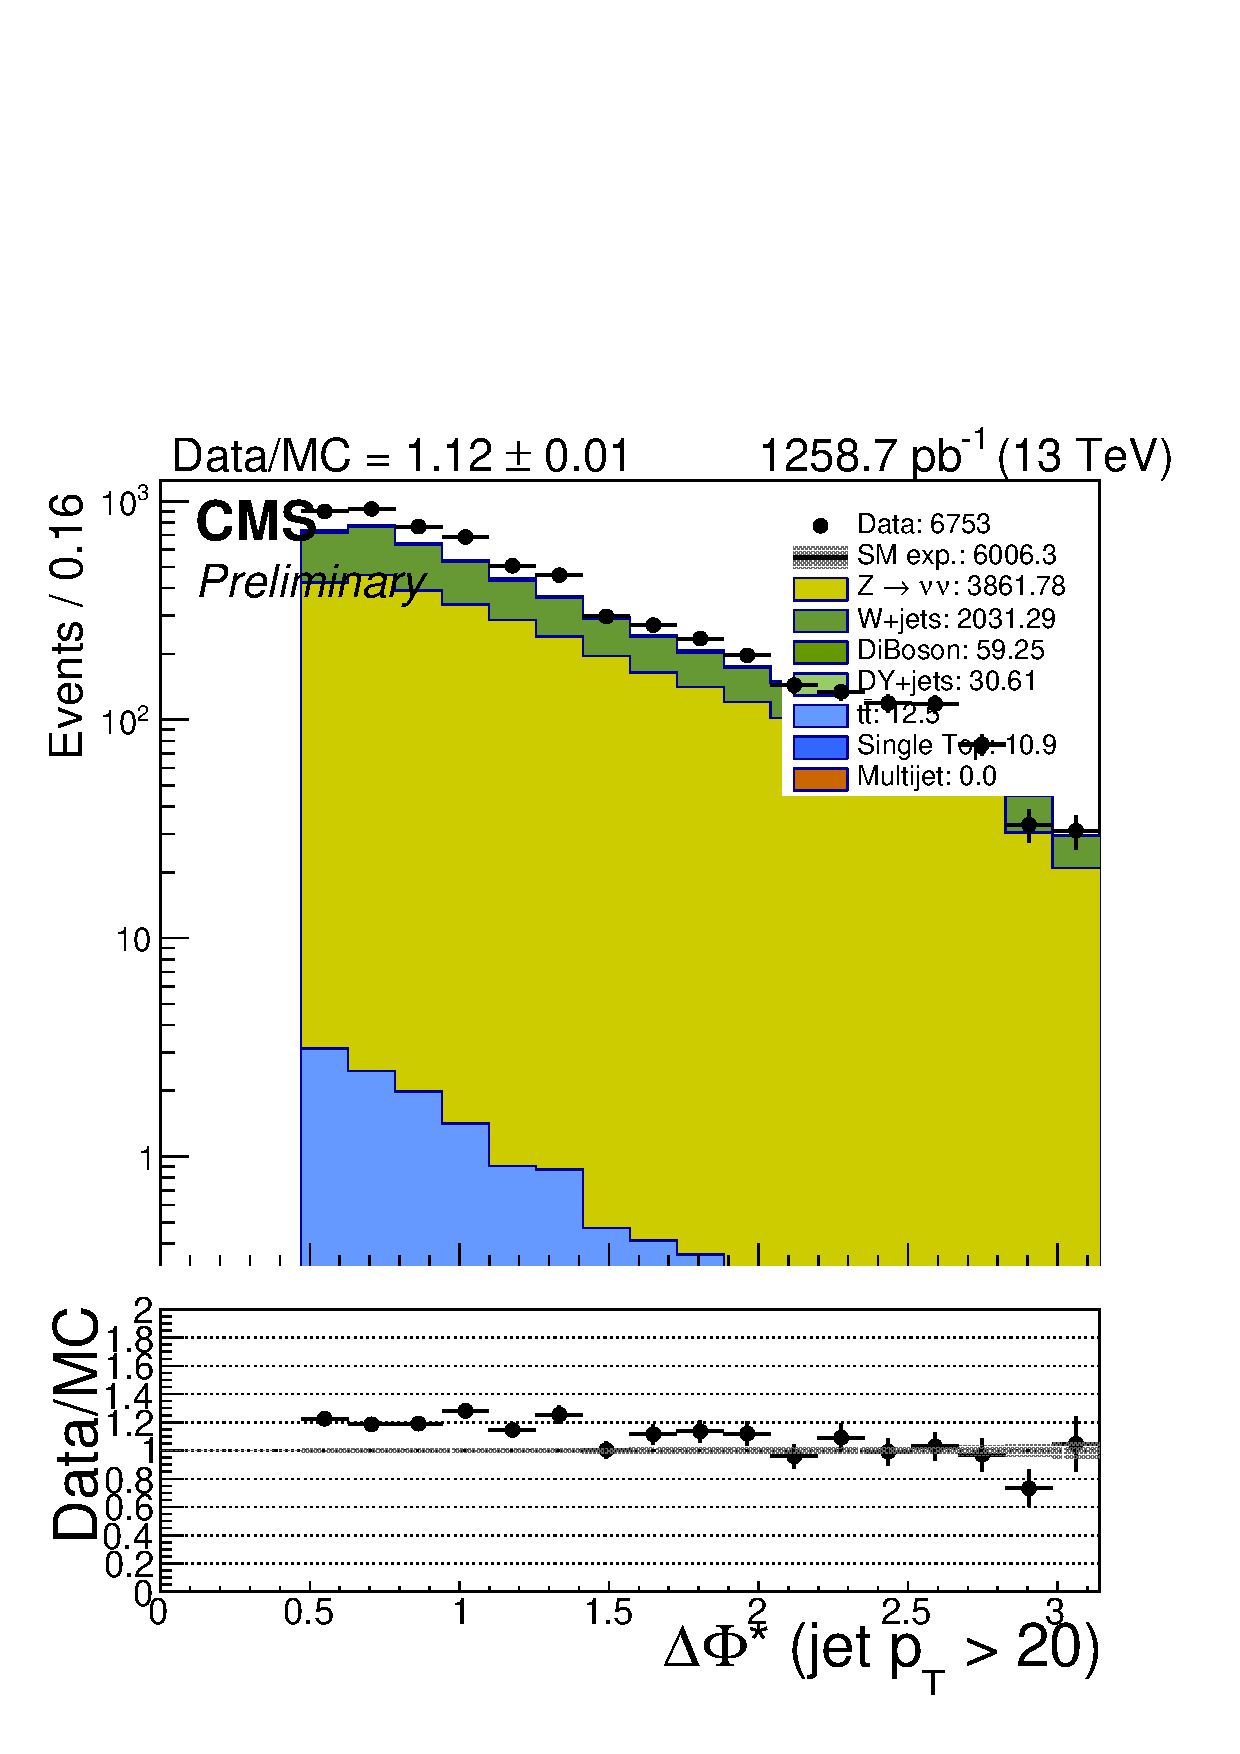
\includegraphics[width=0.5\textwidth]{figures/distributions/Signal/biasedDPhi20_eq1j.pdf}} \\
        \caption{Key analysis variables for hadronic signal region (monojet bins)}
        \label{fig:distribution_signal_mono}
    \end{center}
\end{figure}
%%____________________________________________________________________________||
\begin{figure}
    \begin{center}
        \subfigure {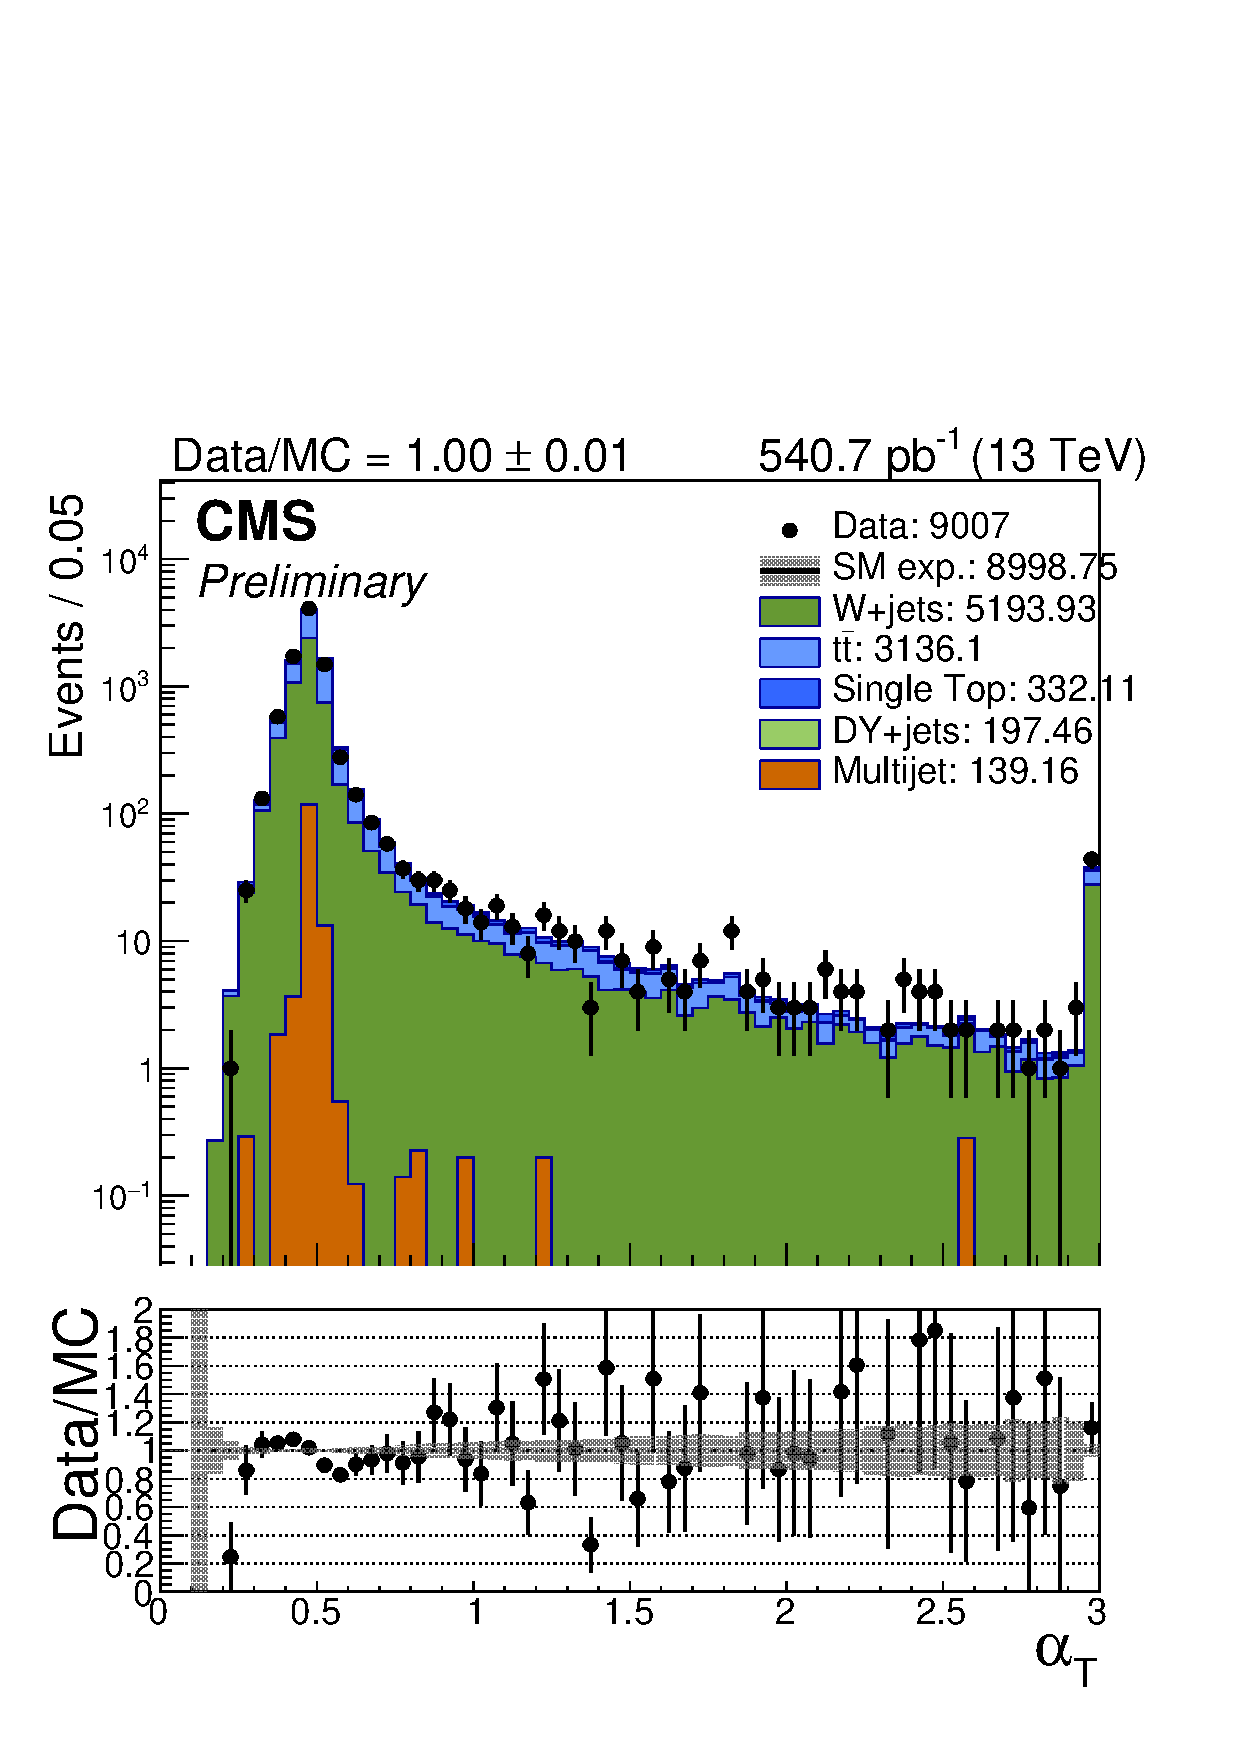
\includegraphics[width=0.5\textwidth]{figures/distributions/SingleMu/alphaT_sym.pdf}} ~~
        \subfigure {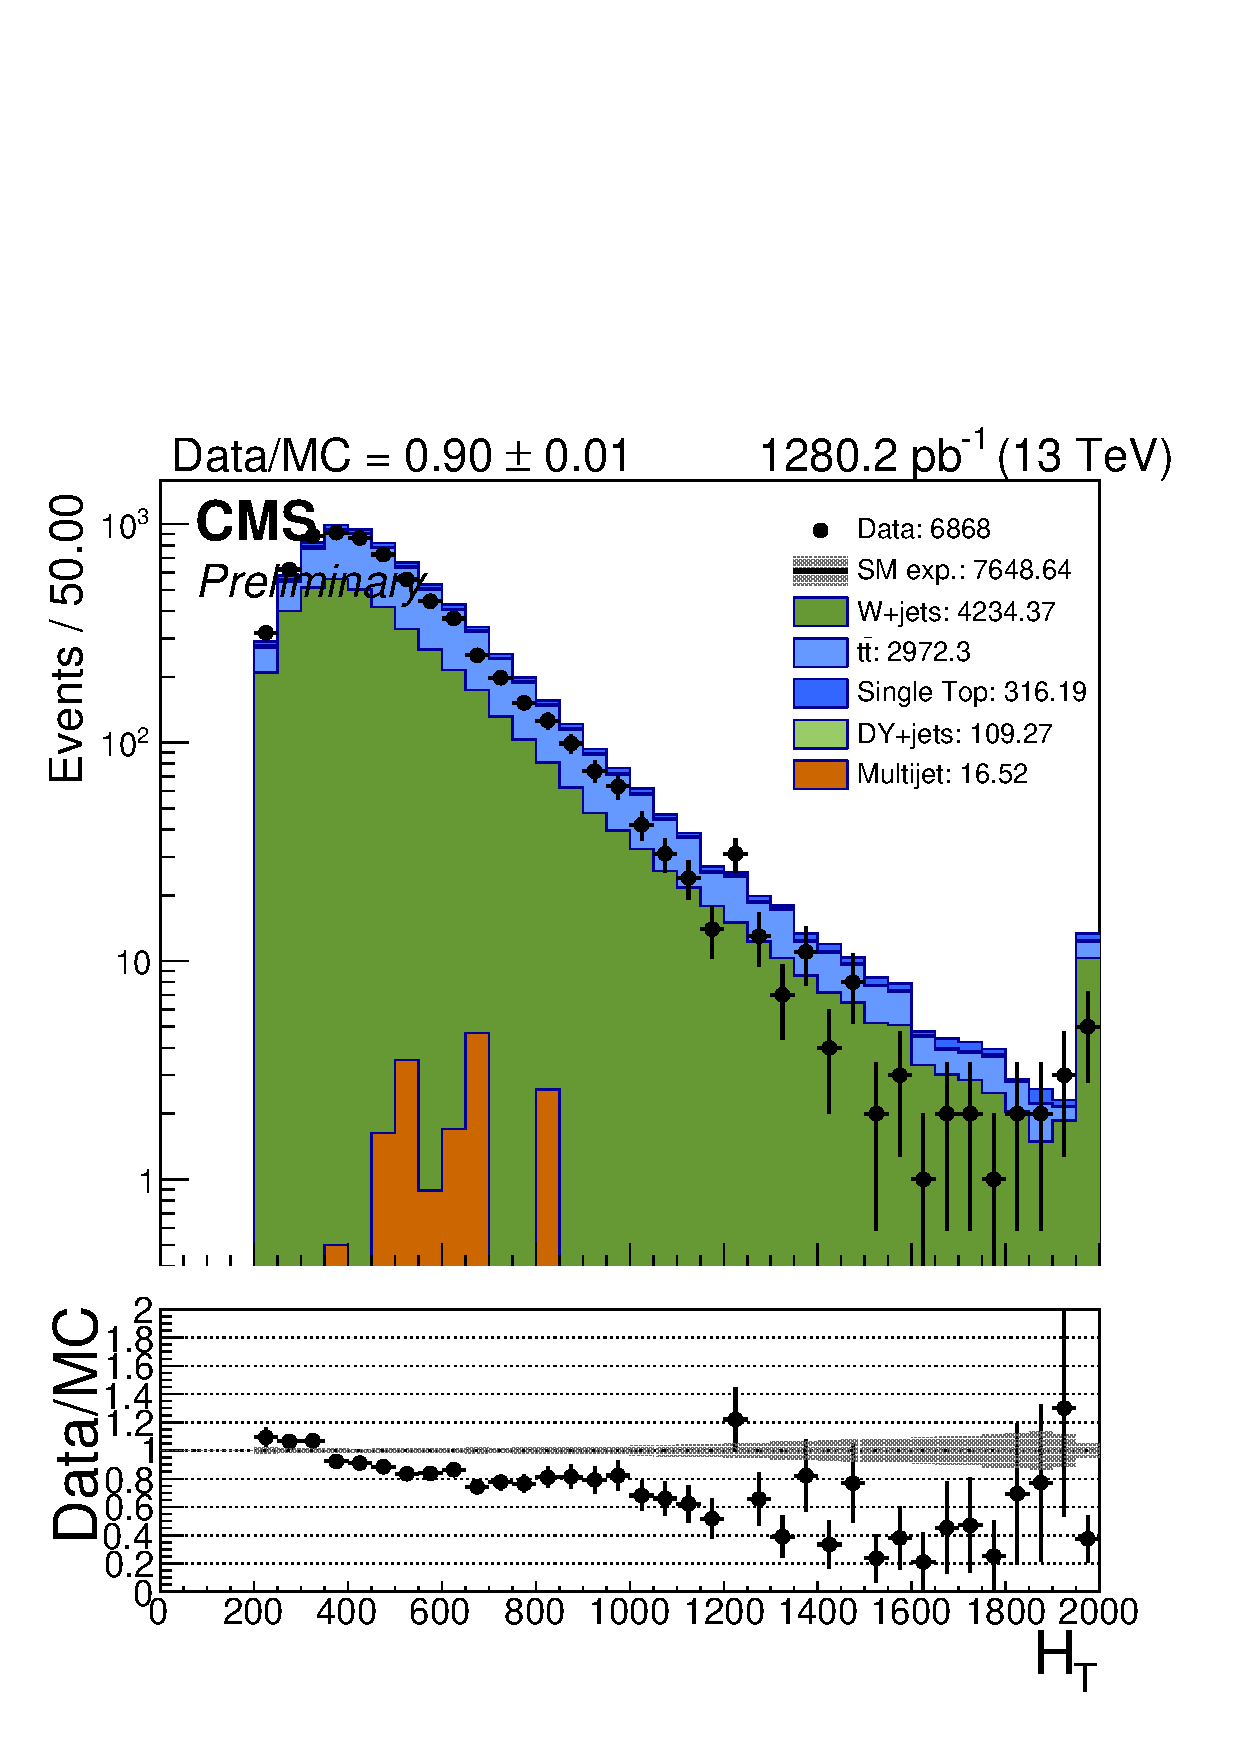
\includegraphics[width=0.5\textwidth]{figures/distributions/SingleMu/ht40_sym.pdf}} \\
        \subfigure {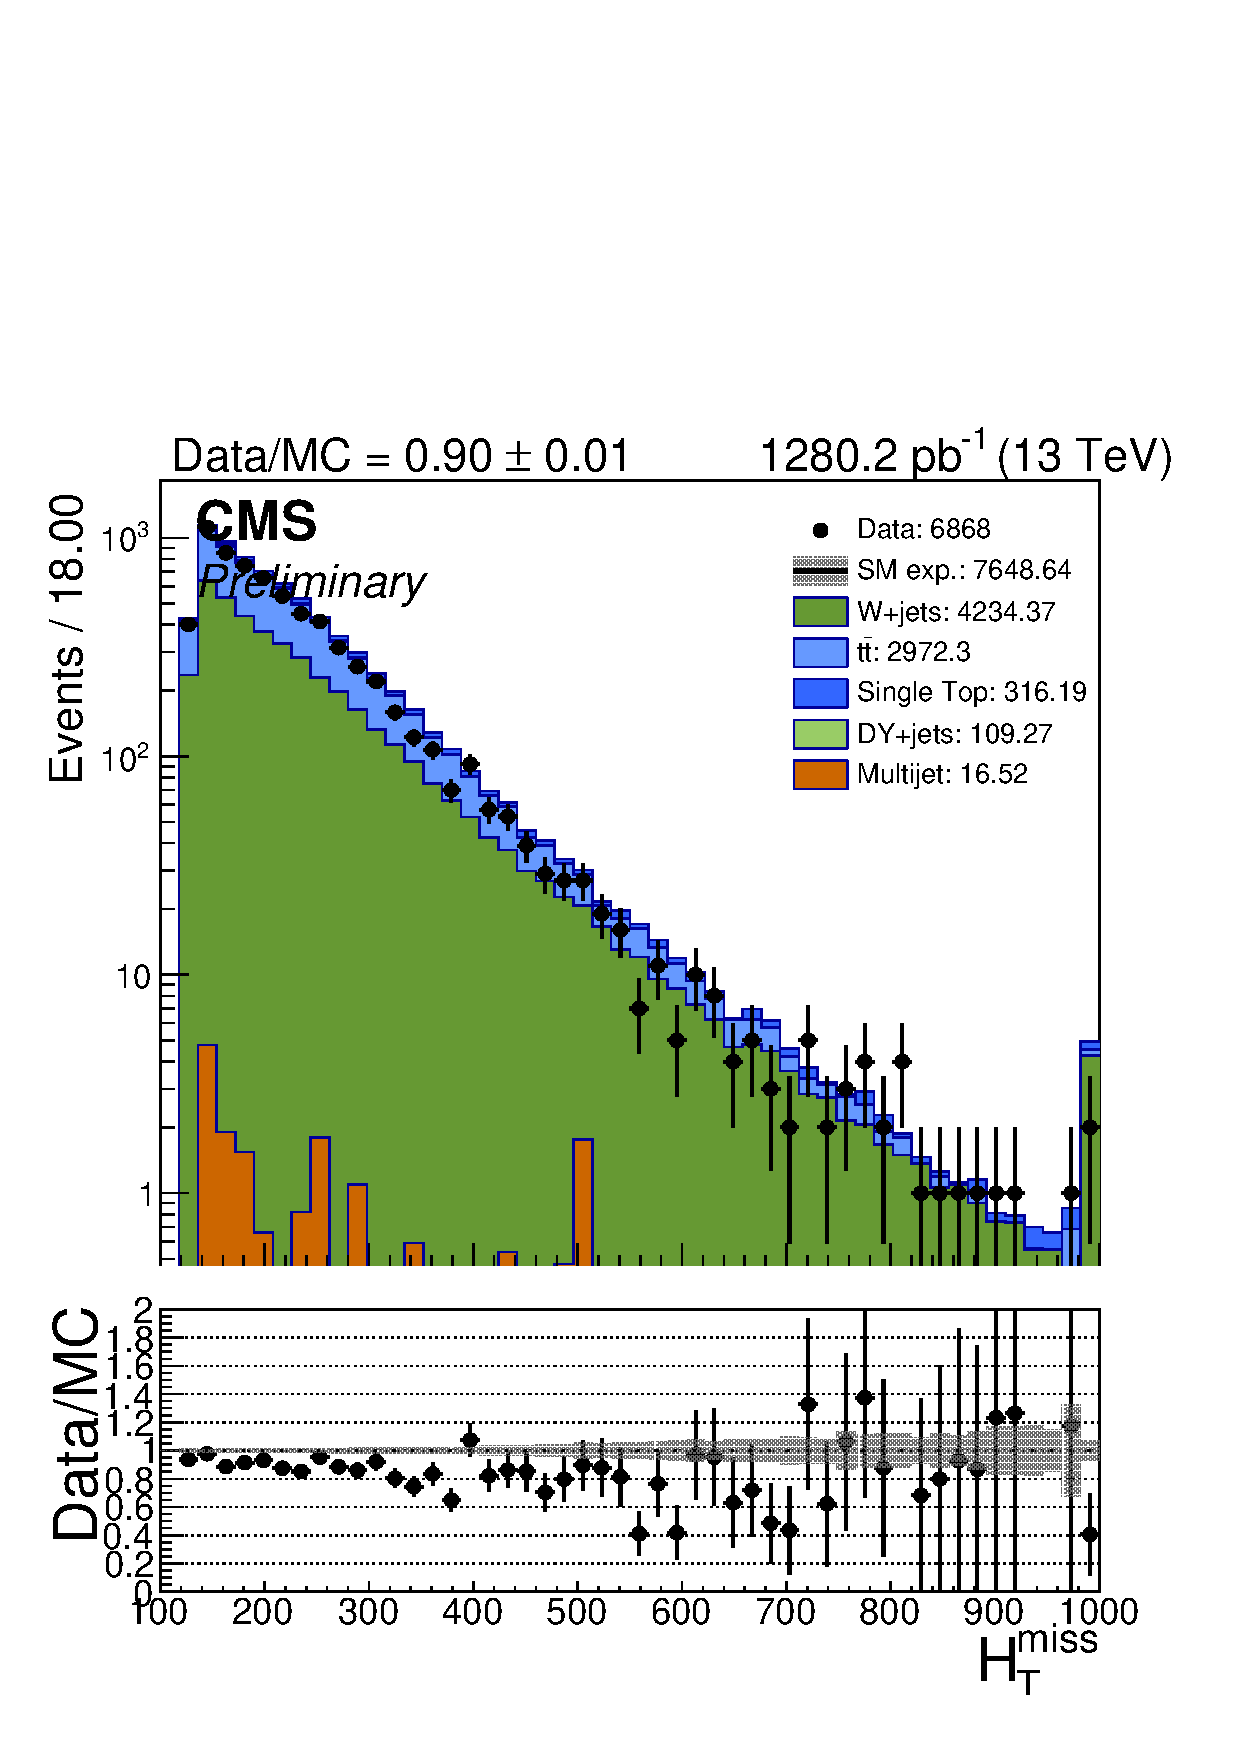
\includegraphics[width=0.5\textwidth]{figures/distributions/SingleMu/mht40_pt_sym.pdf}} ~~
        \subfigure {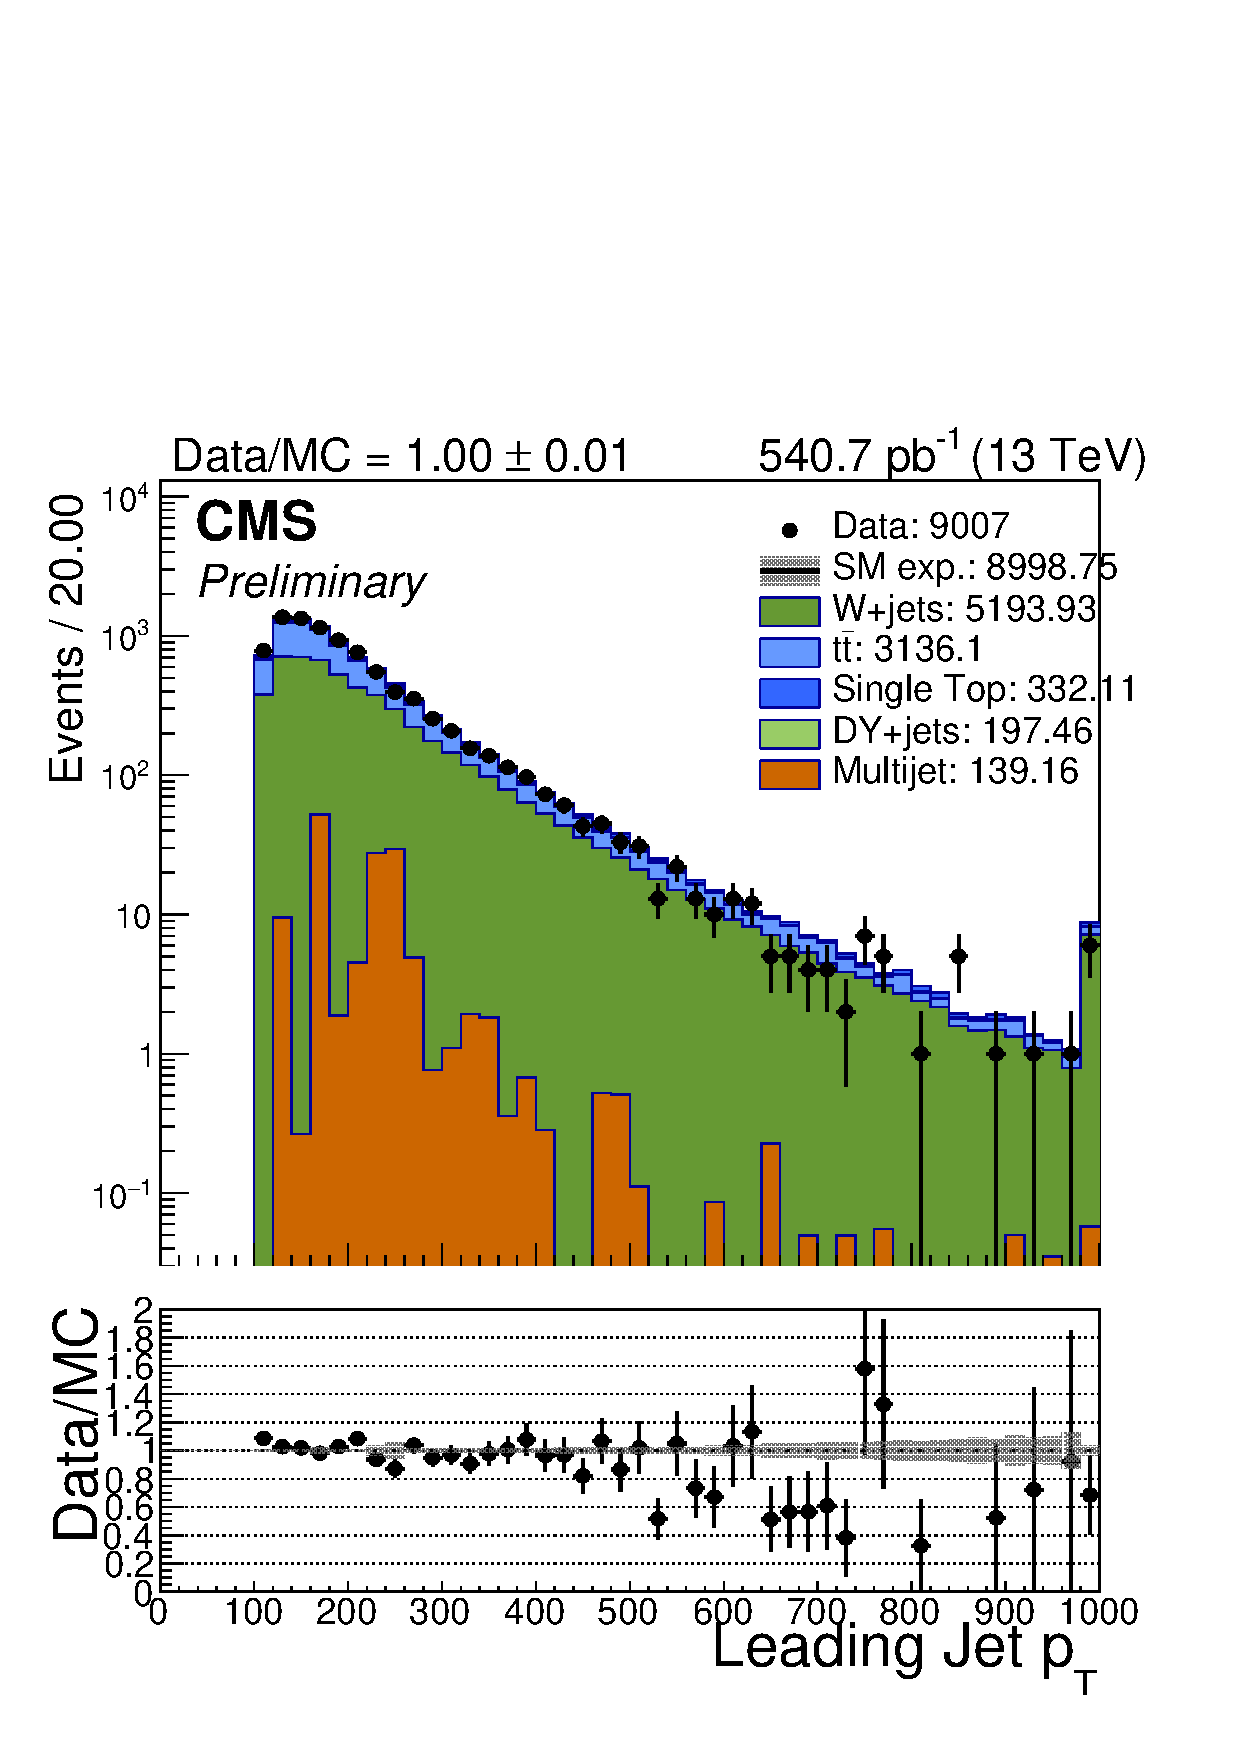
\includegraphics[width=0.5\textwidth]{figures/distributions/SingleMu/jet_pt[0]_sym.pdf}} \\
        \caption{Key analysis variables for single muon control region (symmetric bins)}
        \label{fig:distribution_singlemu_sym}
    \end{center}
\end{figure}

\begin{figure}
    \begin{center}
        \subfigure {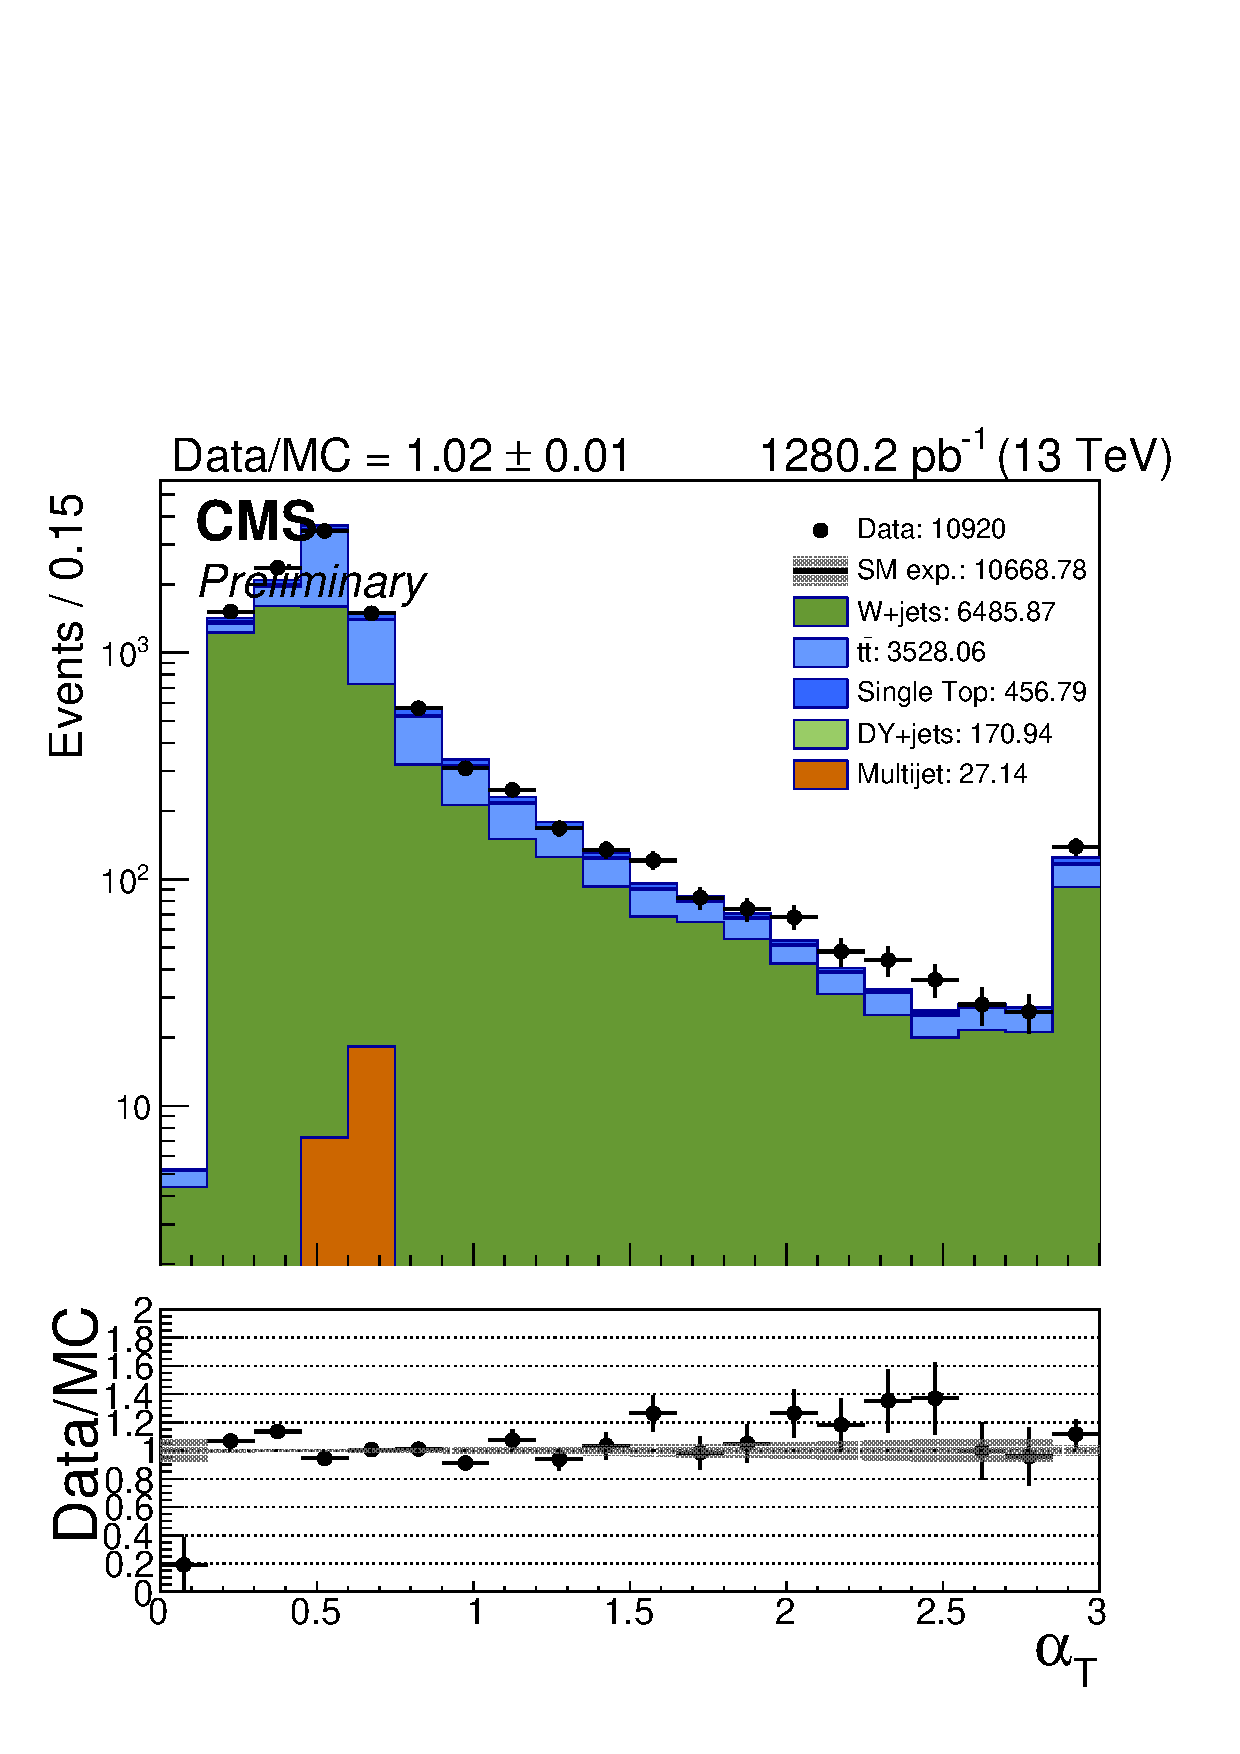
\includegraphics[width=0.5\textwidth]{figures/distributions/SingleMu/alphaT_asym.pdf}} ~~
        \subfigure {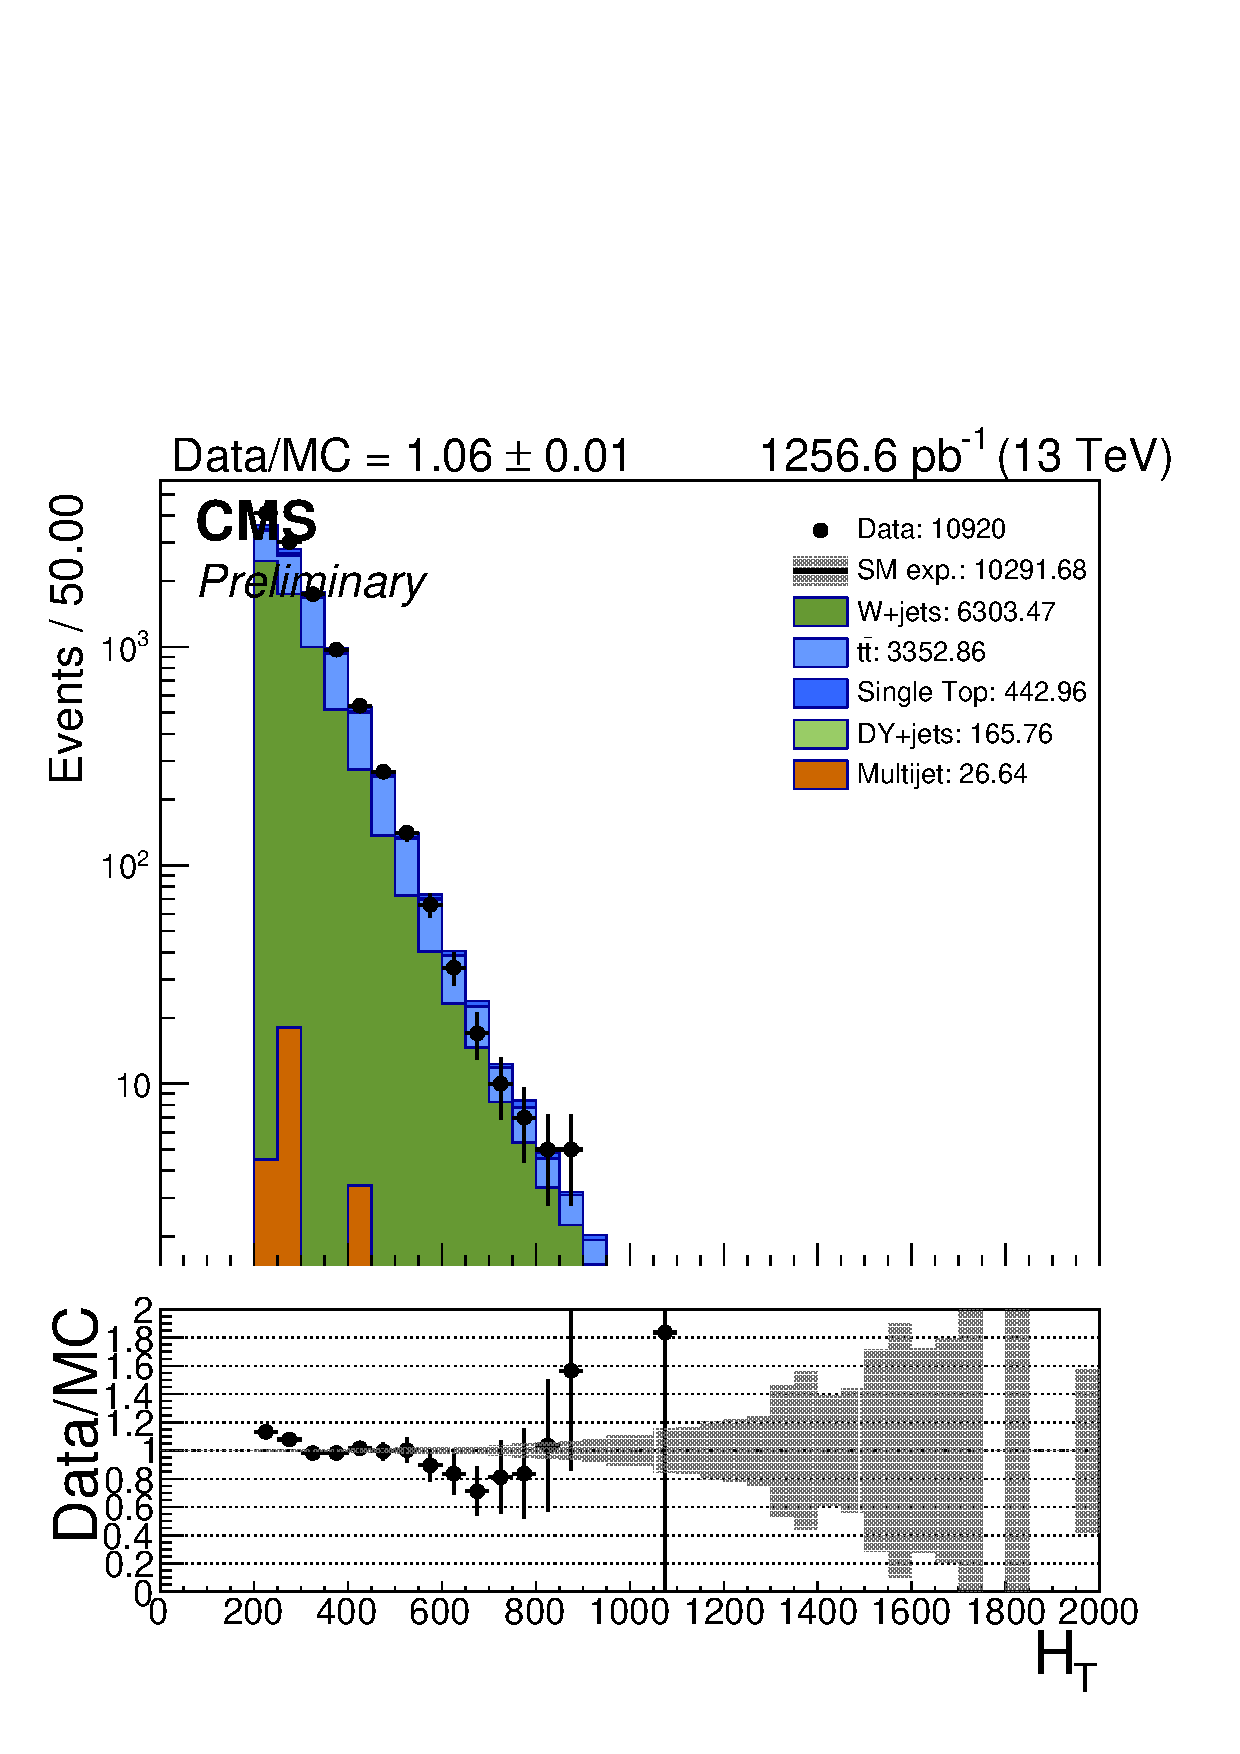
\includegraphics[width=0.5\textwidth]{figures/distributions/SingleMu/ht40_asym.pdf}} \\
        \subfigure {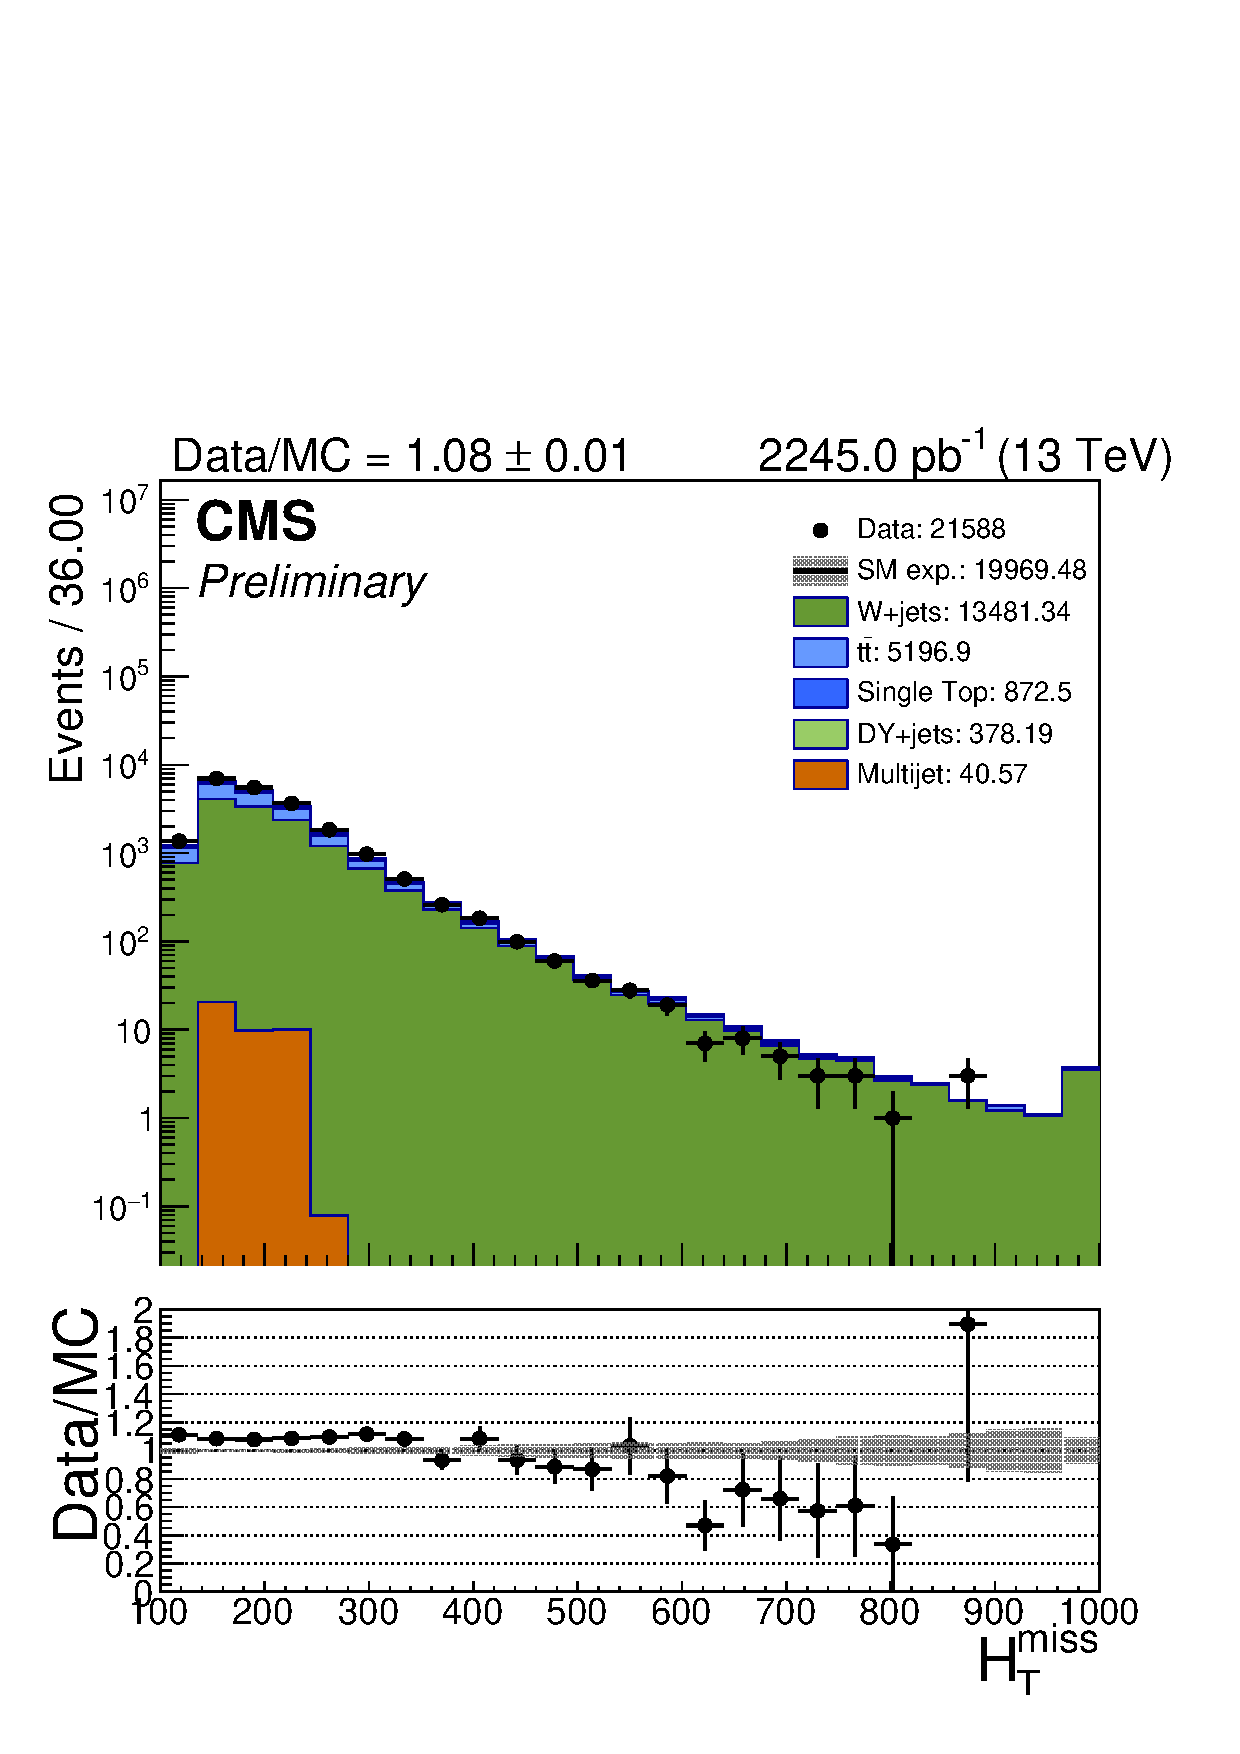
\includegraphics[width=0.5\textwidth]{figures/distributions/SingleMu/mht40_pt_asym.pdf}} ~~
        \subfigure {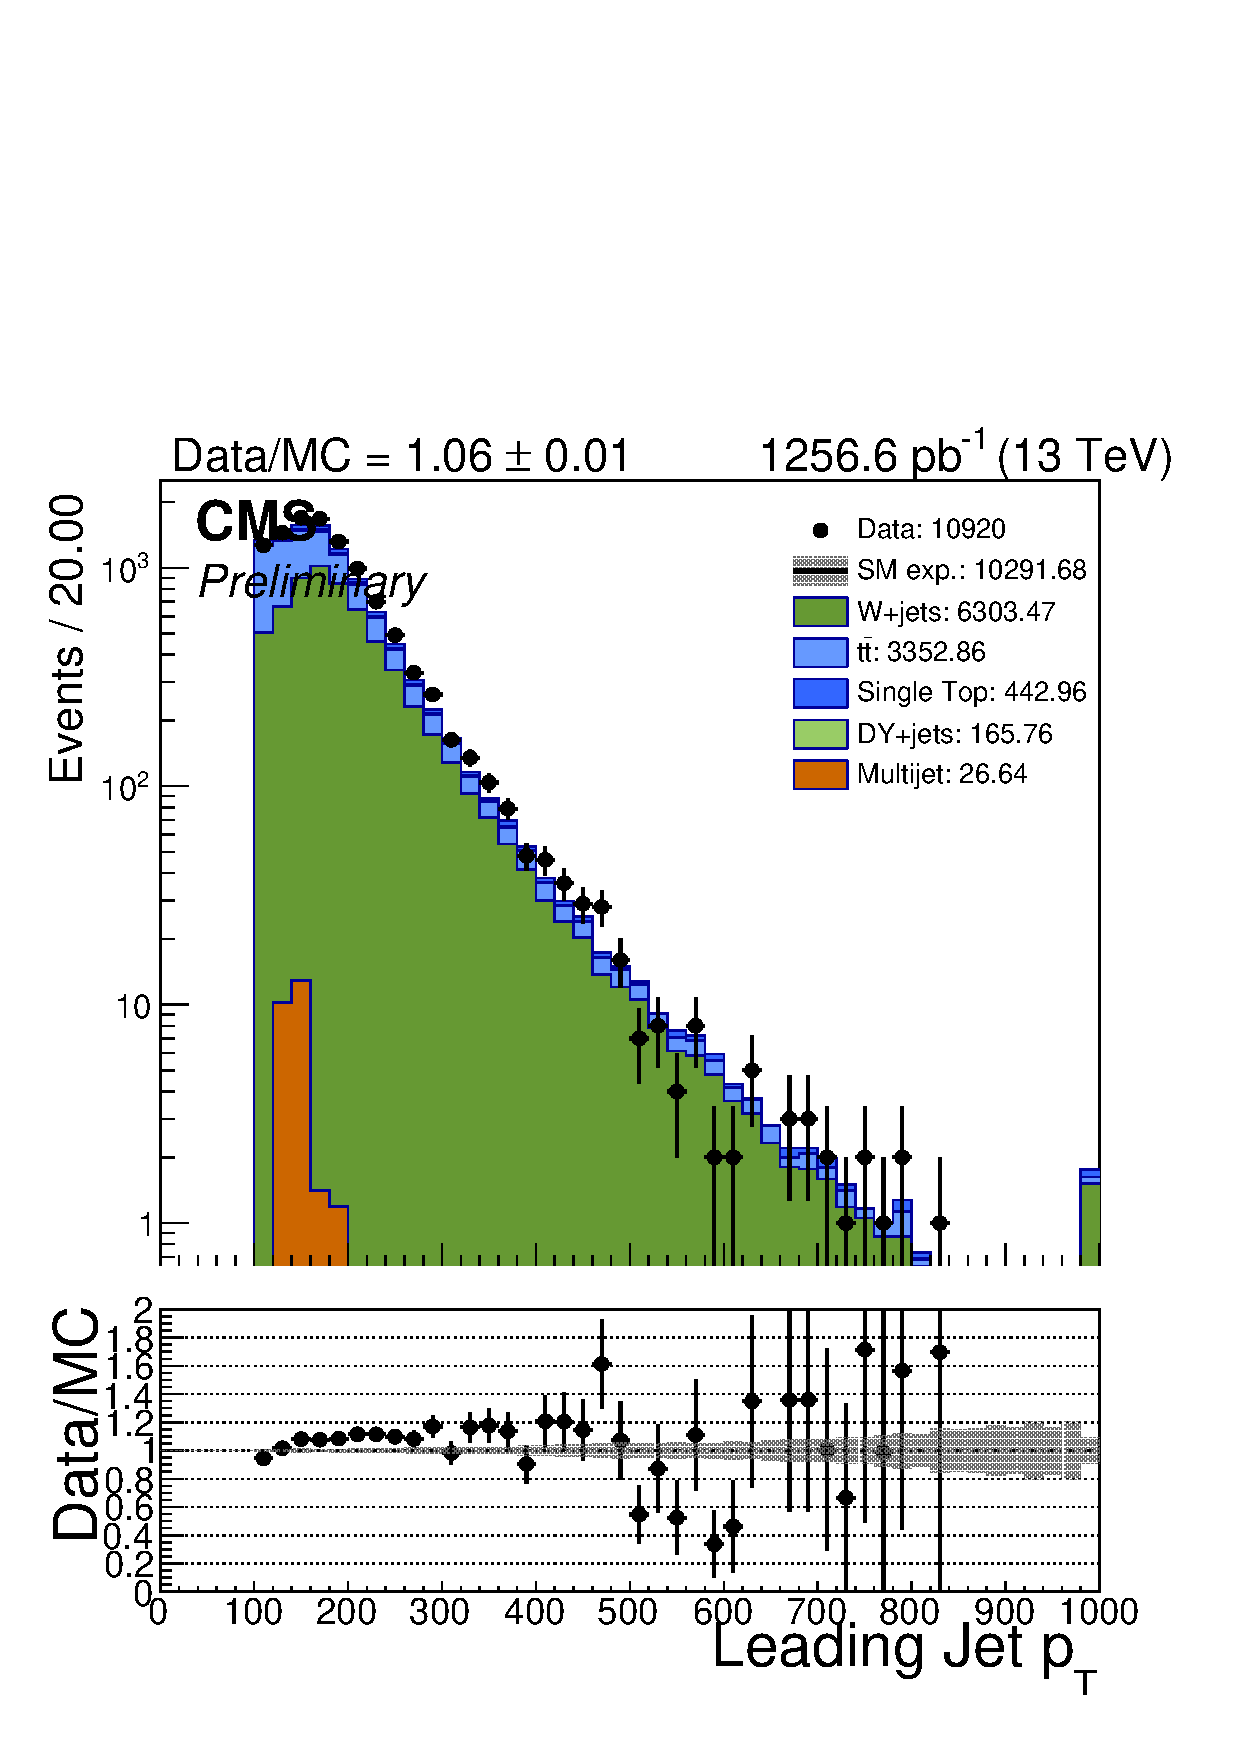
\includegraphics[width=0.5\textwidth]{figures/distributions/SingleMu/jet_pt[0]_asym.pdf}} \\
        \caption{Key analysis variables for single muon control region (asymmetric bins)}
        \label{fig:distribution_singlemu_asym}
    \end{center}
\end{figure}

\begin{figure}
    \begin{center}
        
        \subfigure {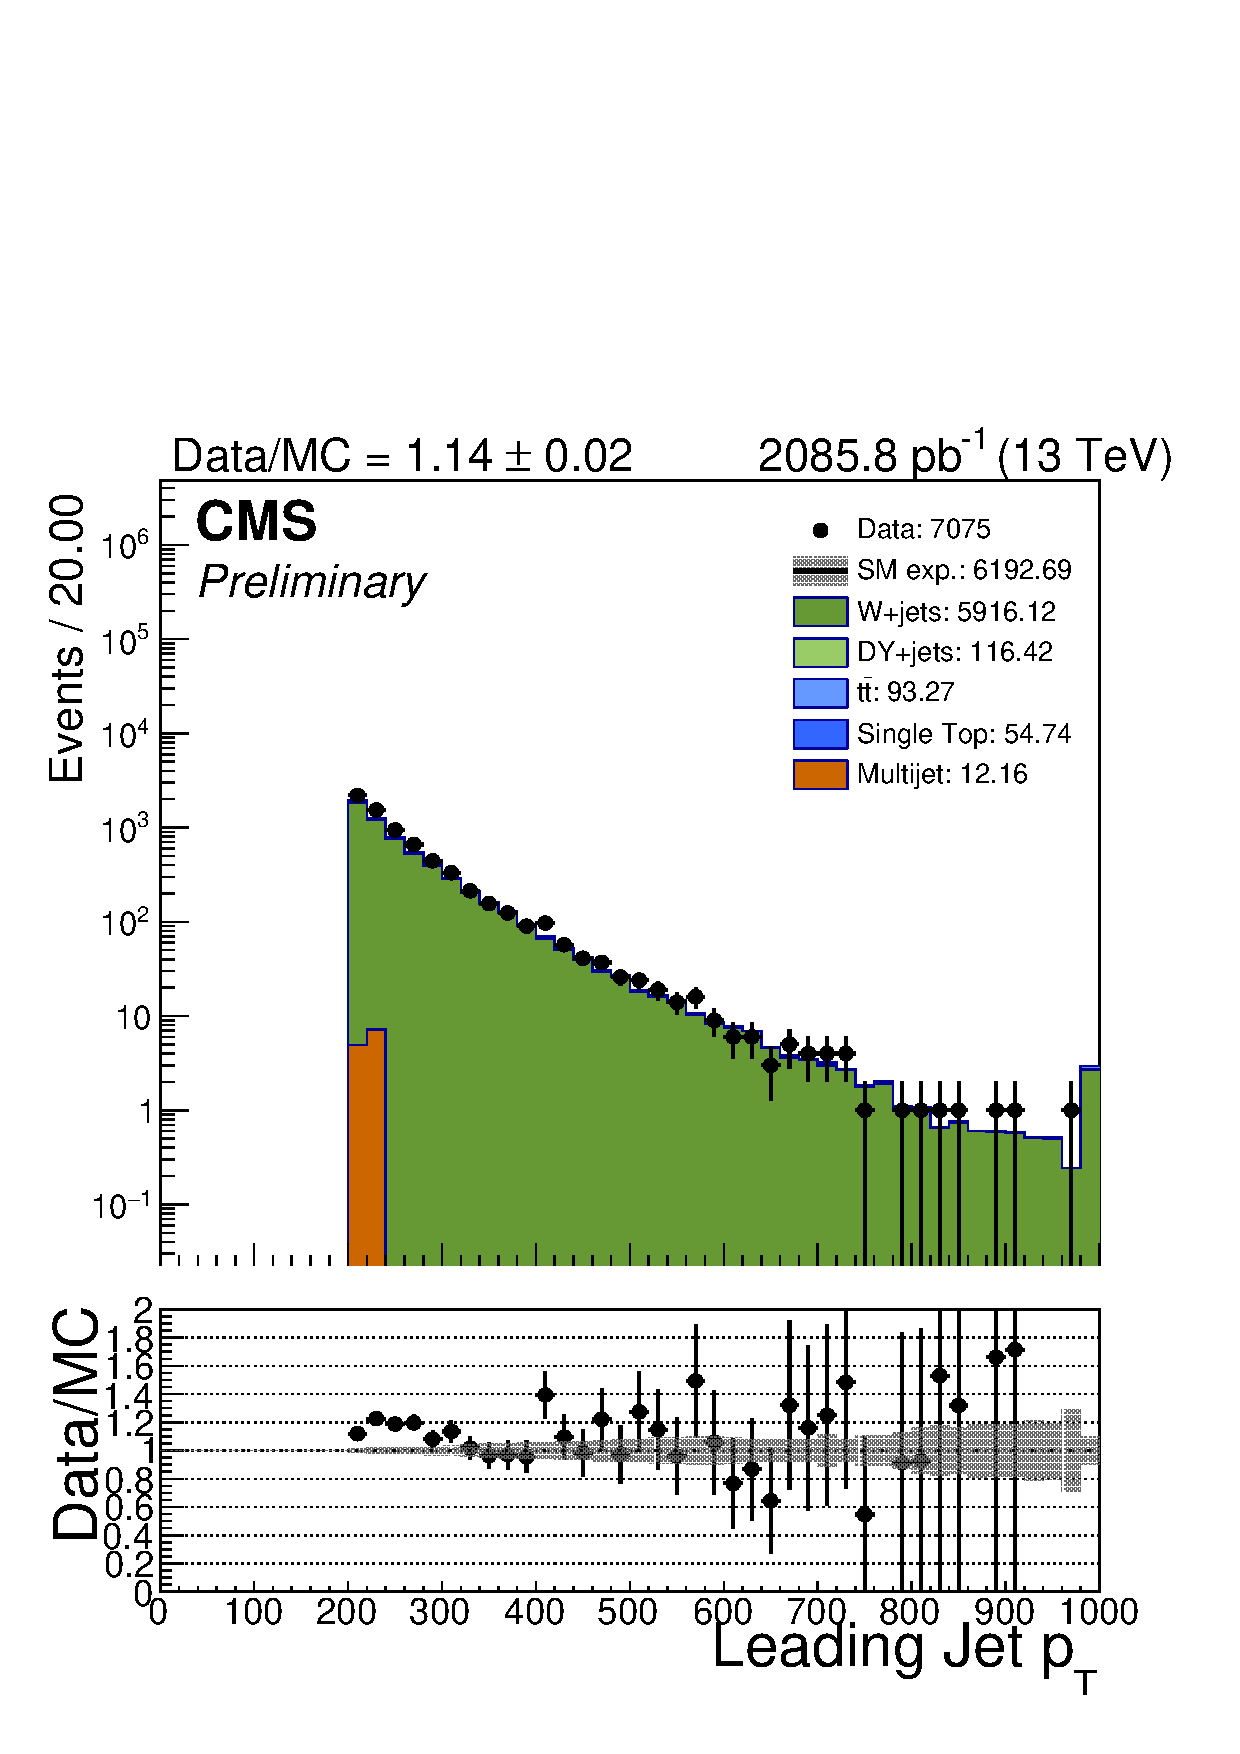
\includegraphics[width=0.5\textwidth]{figures/distributions/SingleMu/jet_pt[0]_eq1j.pdf}} ~~
        \subfigure {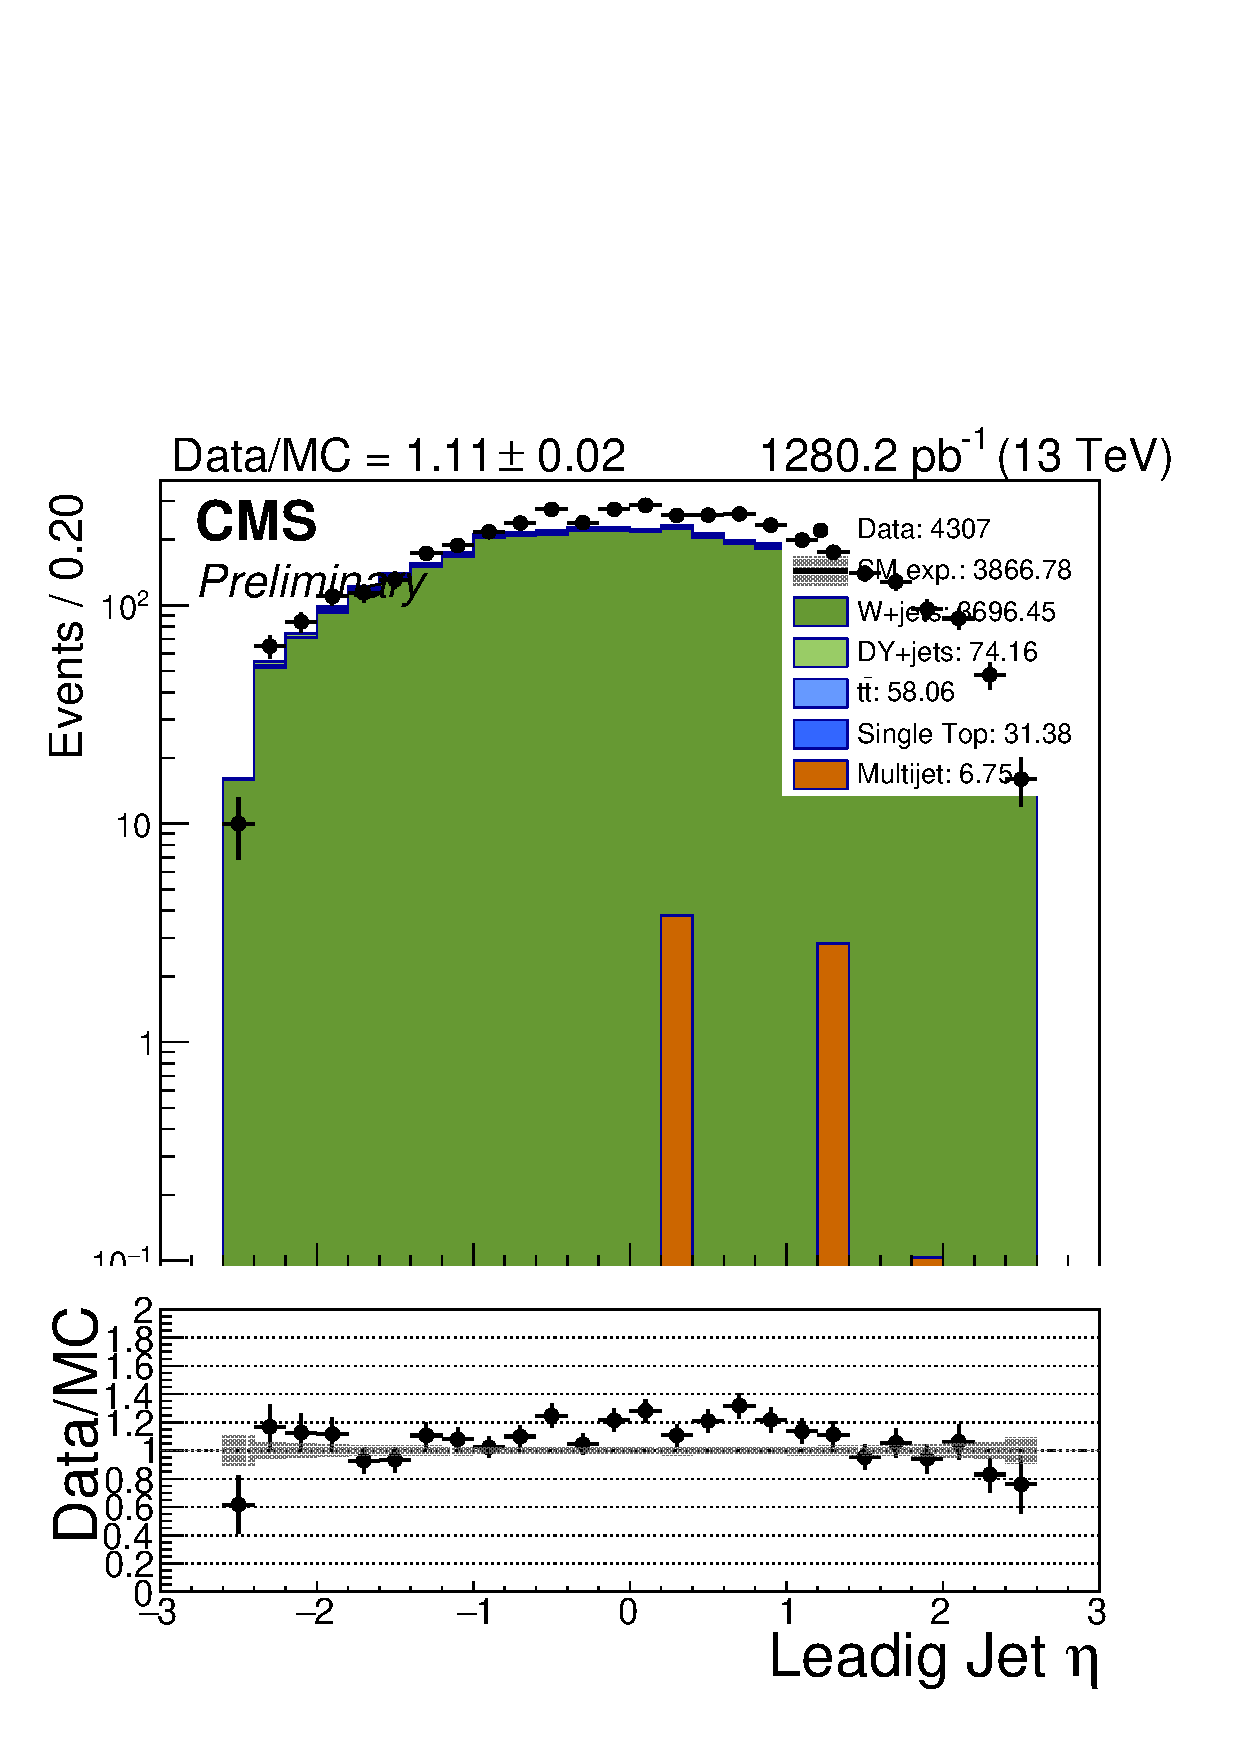
\includegraphics[width=0.5\textwidth]{figures/distributions/SingleMu/jet_eta[0]_eq1j.pdf}} \\
        \subfigure {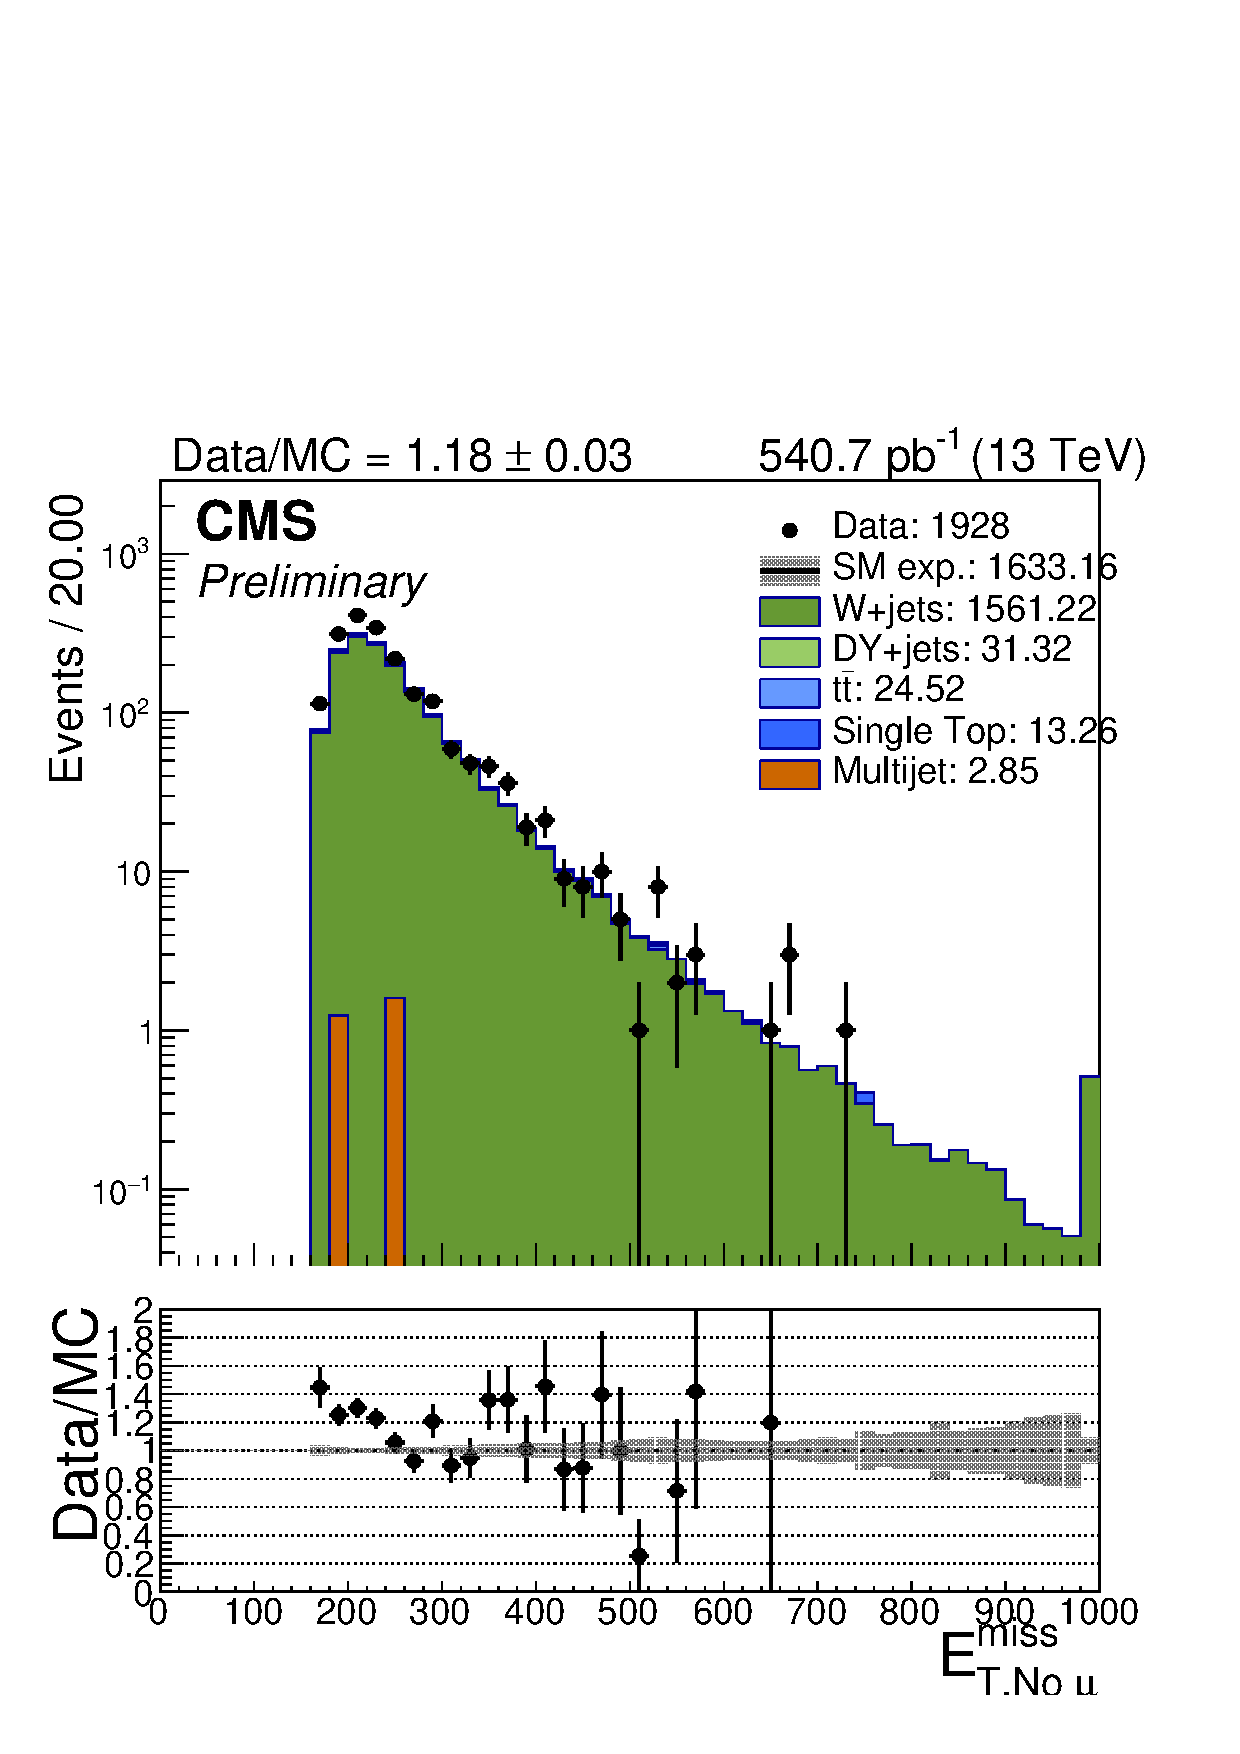
\includegraphics[width=0.5\textwidth]{figures/distributions/SingleMu/metNoMu_pt_eq1j.pdf}} ~~
        \subfigure {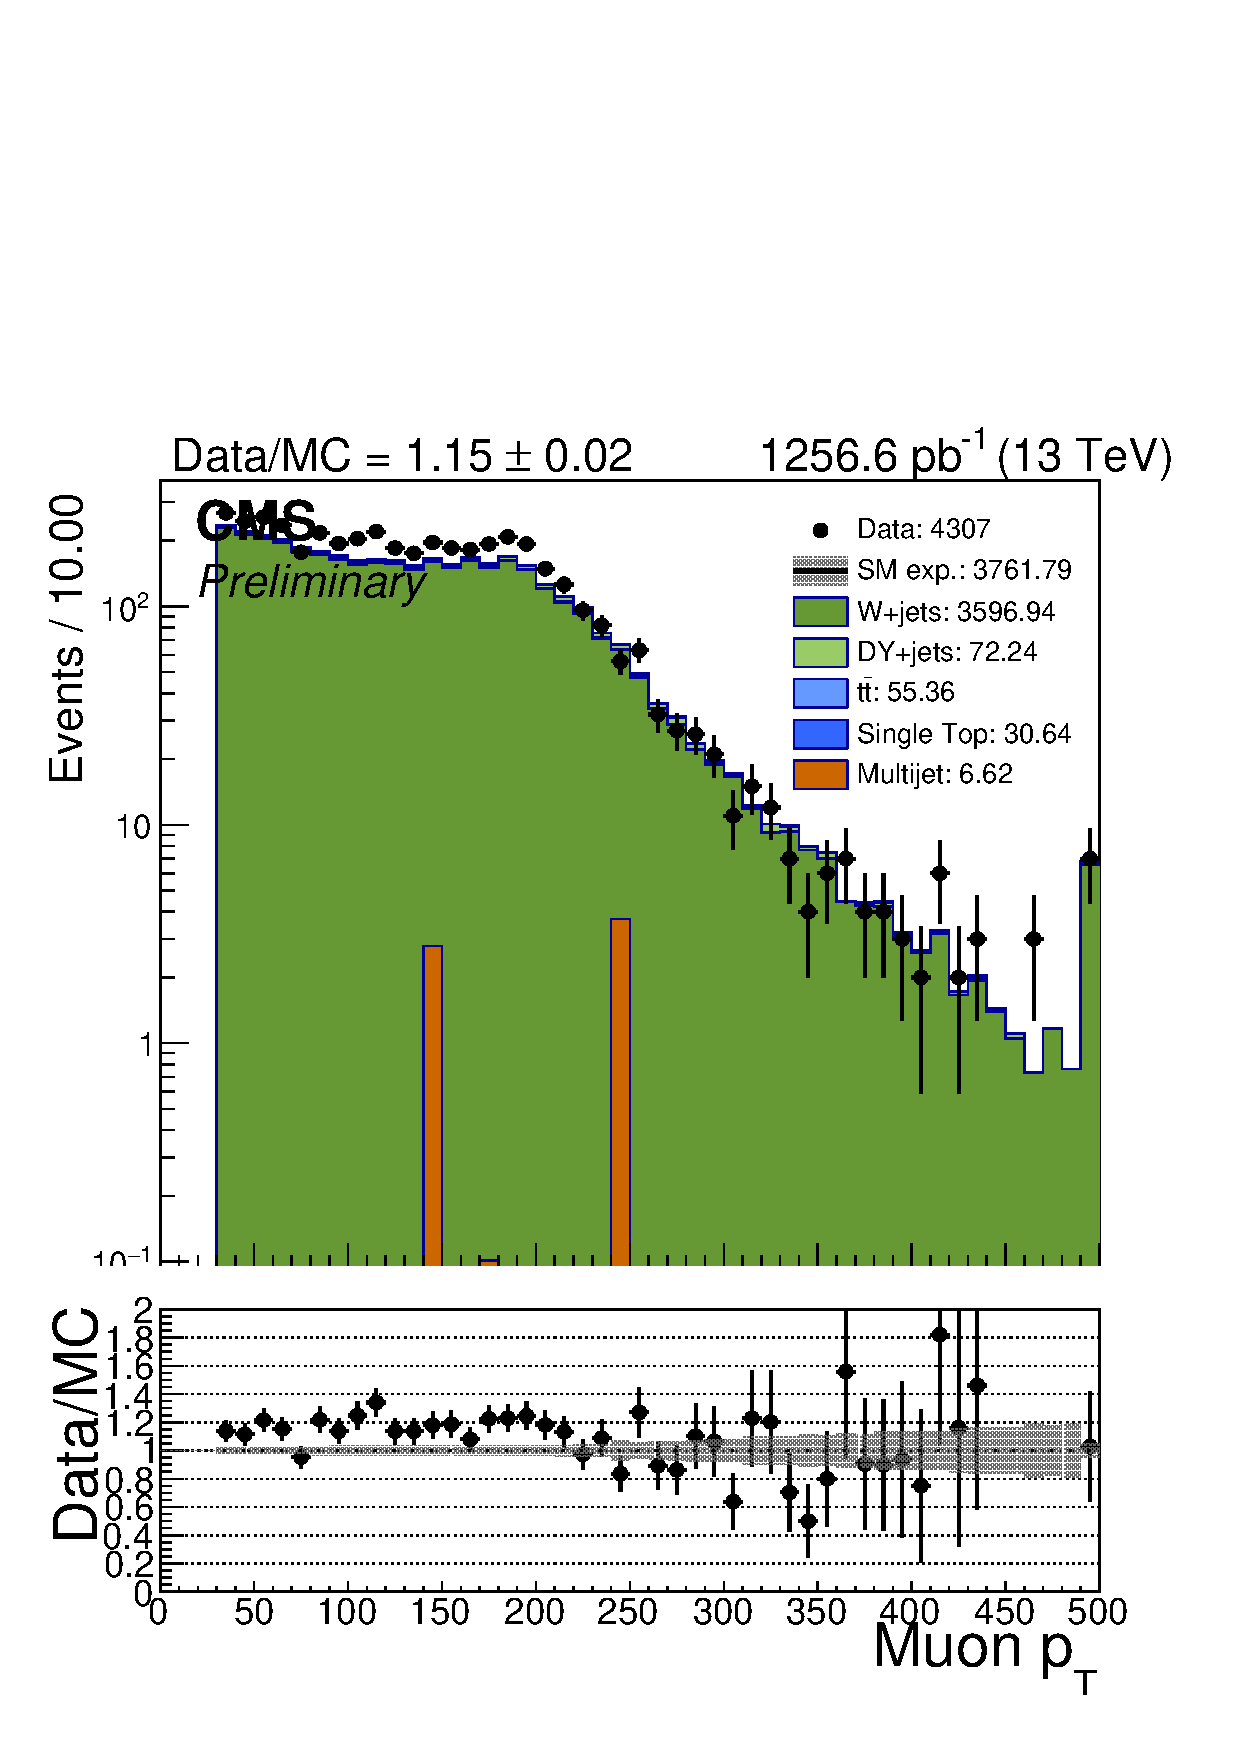
\includegraphics[width=0.5\textwidth]{figures/distributions/SingleMu/muon_pt[0]_eq1j.pdf}} \\
        \caption{Key analysis variables for single muon control region (monojet bins)}
        \label{fig:distribution_singlemu_mono}
    \end{center}
\end{figure}
%%____________________________________________________________________________||
\begin{figure}
    \begin{center}
        \subfigure {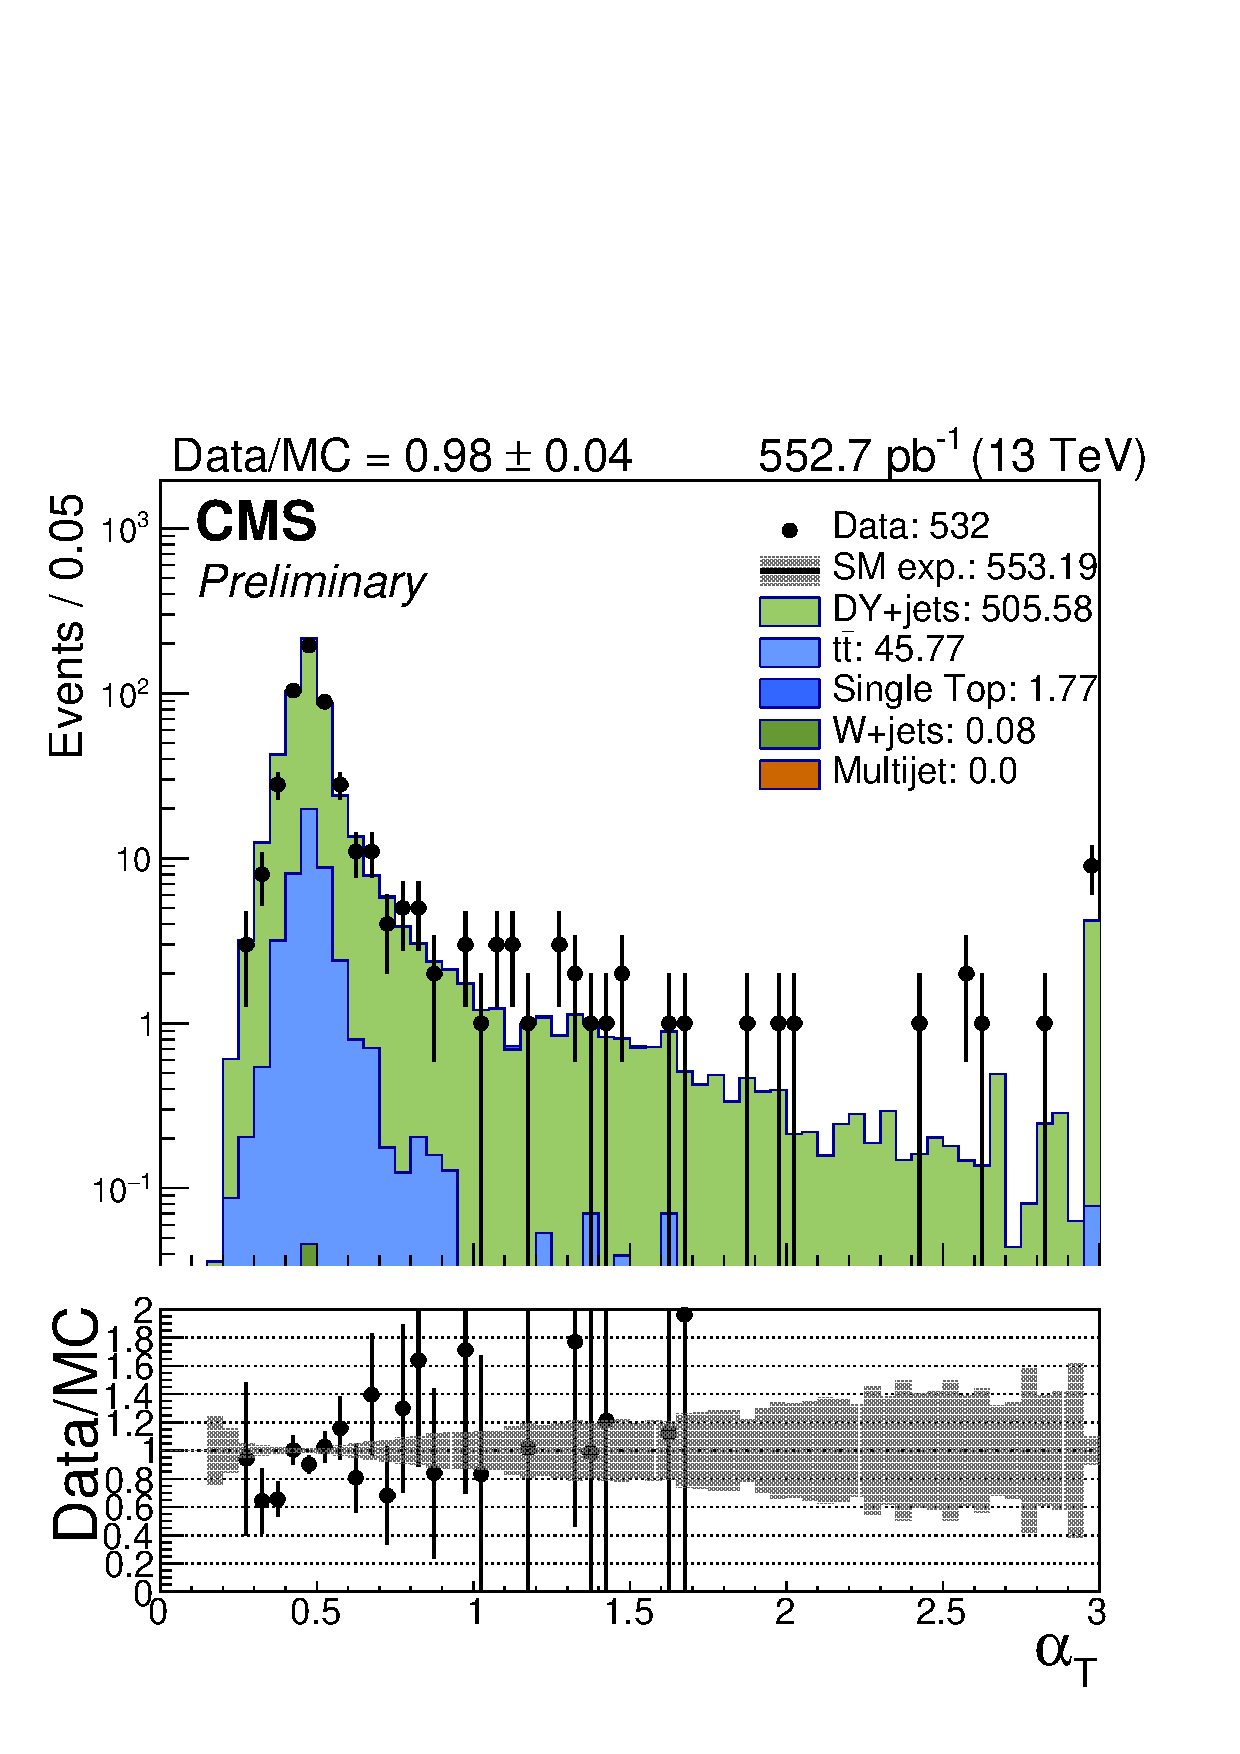
\includegraphics[width=0.5\textwidth]{figures/distributions/DoubleMu/alphaT_sym.pdf}} ~~
        \subfigure {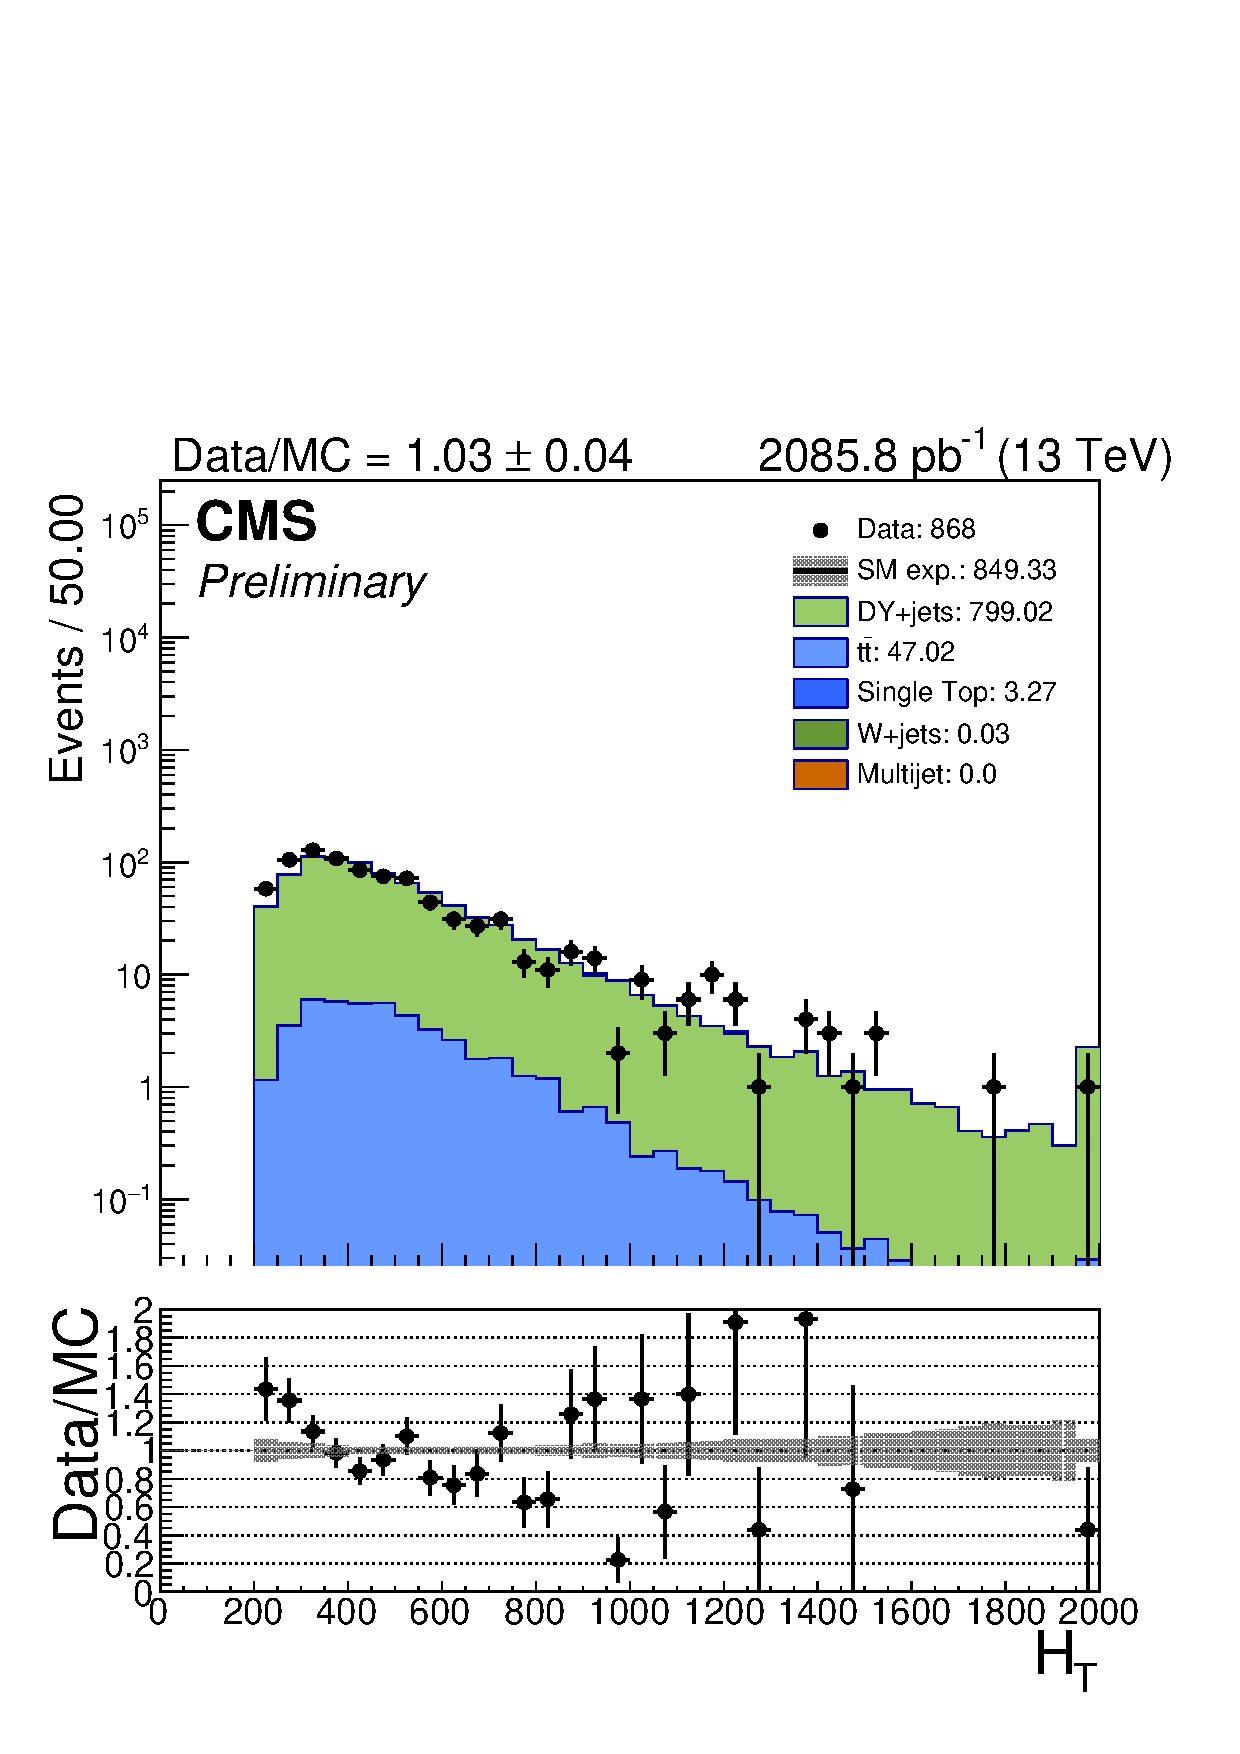
\includegraphics[width=0.5\textwidth]{figures/distributions/DoubleMu/ht40_sym.pdf}} \\
        \subfigure {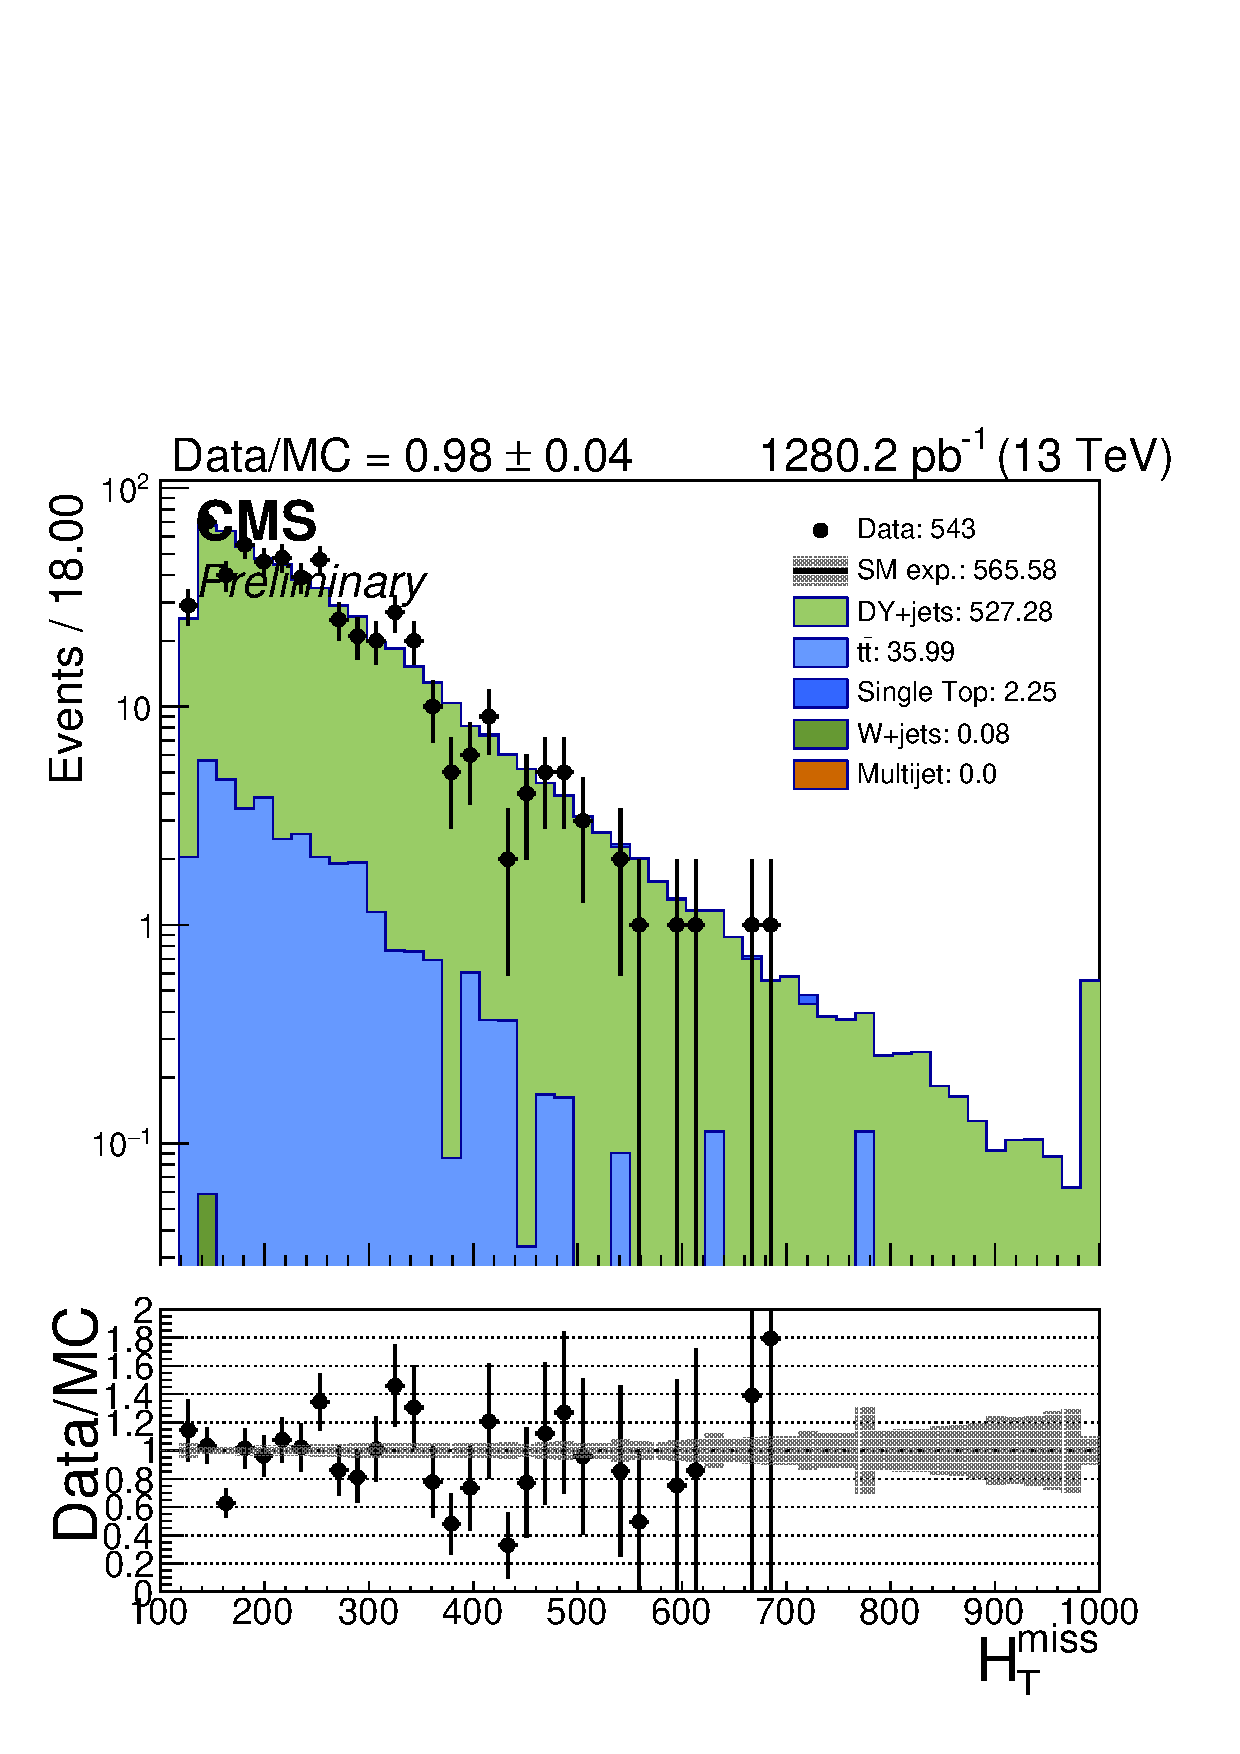
\includegraphics[width=0.5\textwidth]{figures/distributions/DoubleMu/mht40_pt_sym.pdf}} ~~
        \subfigure {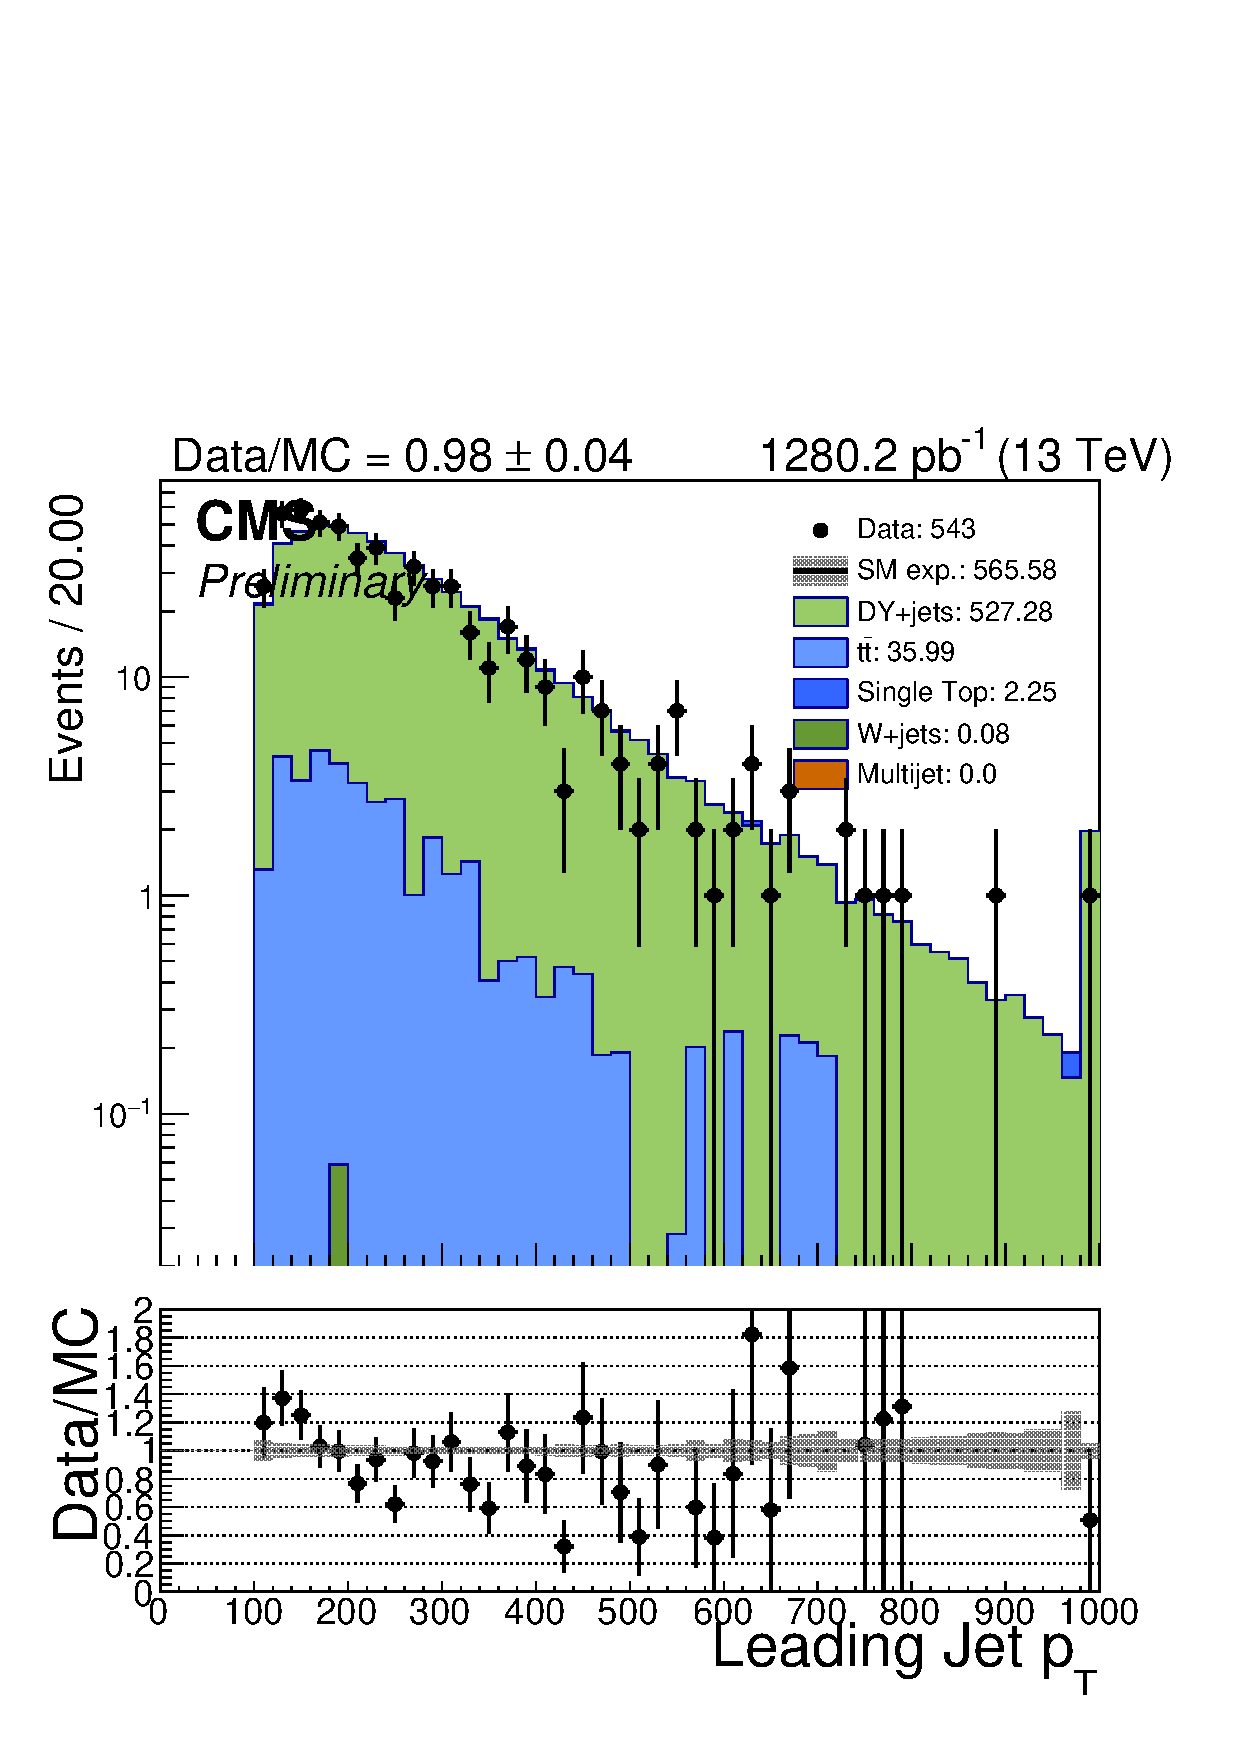
\includegraphics[width=0.5\textwidth]{figures/distributions/DoubleMu/jet_pt[0]_sym.pdf}} \\
        \caption{Key analysis variables for double muon control region (symmetric bins)}
        \label{fig:distribution_doublemu_sym}
    \end{center}
\end{figure}

\begin{figure}
    \begin{center}
        \subfigure {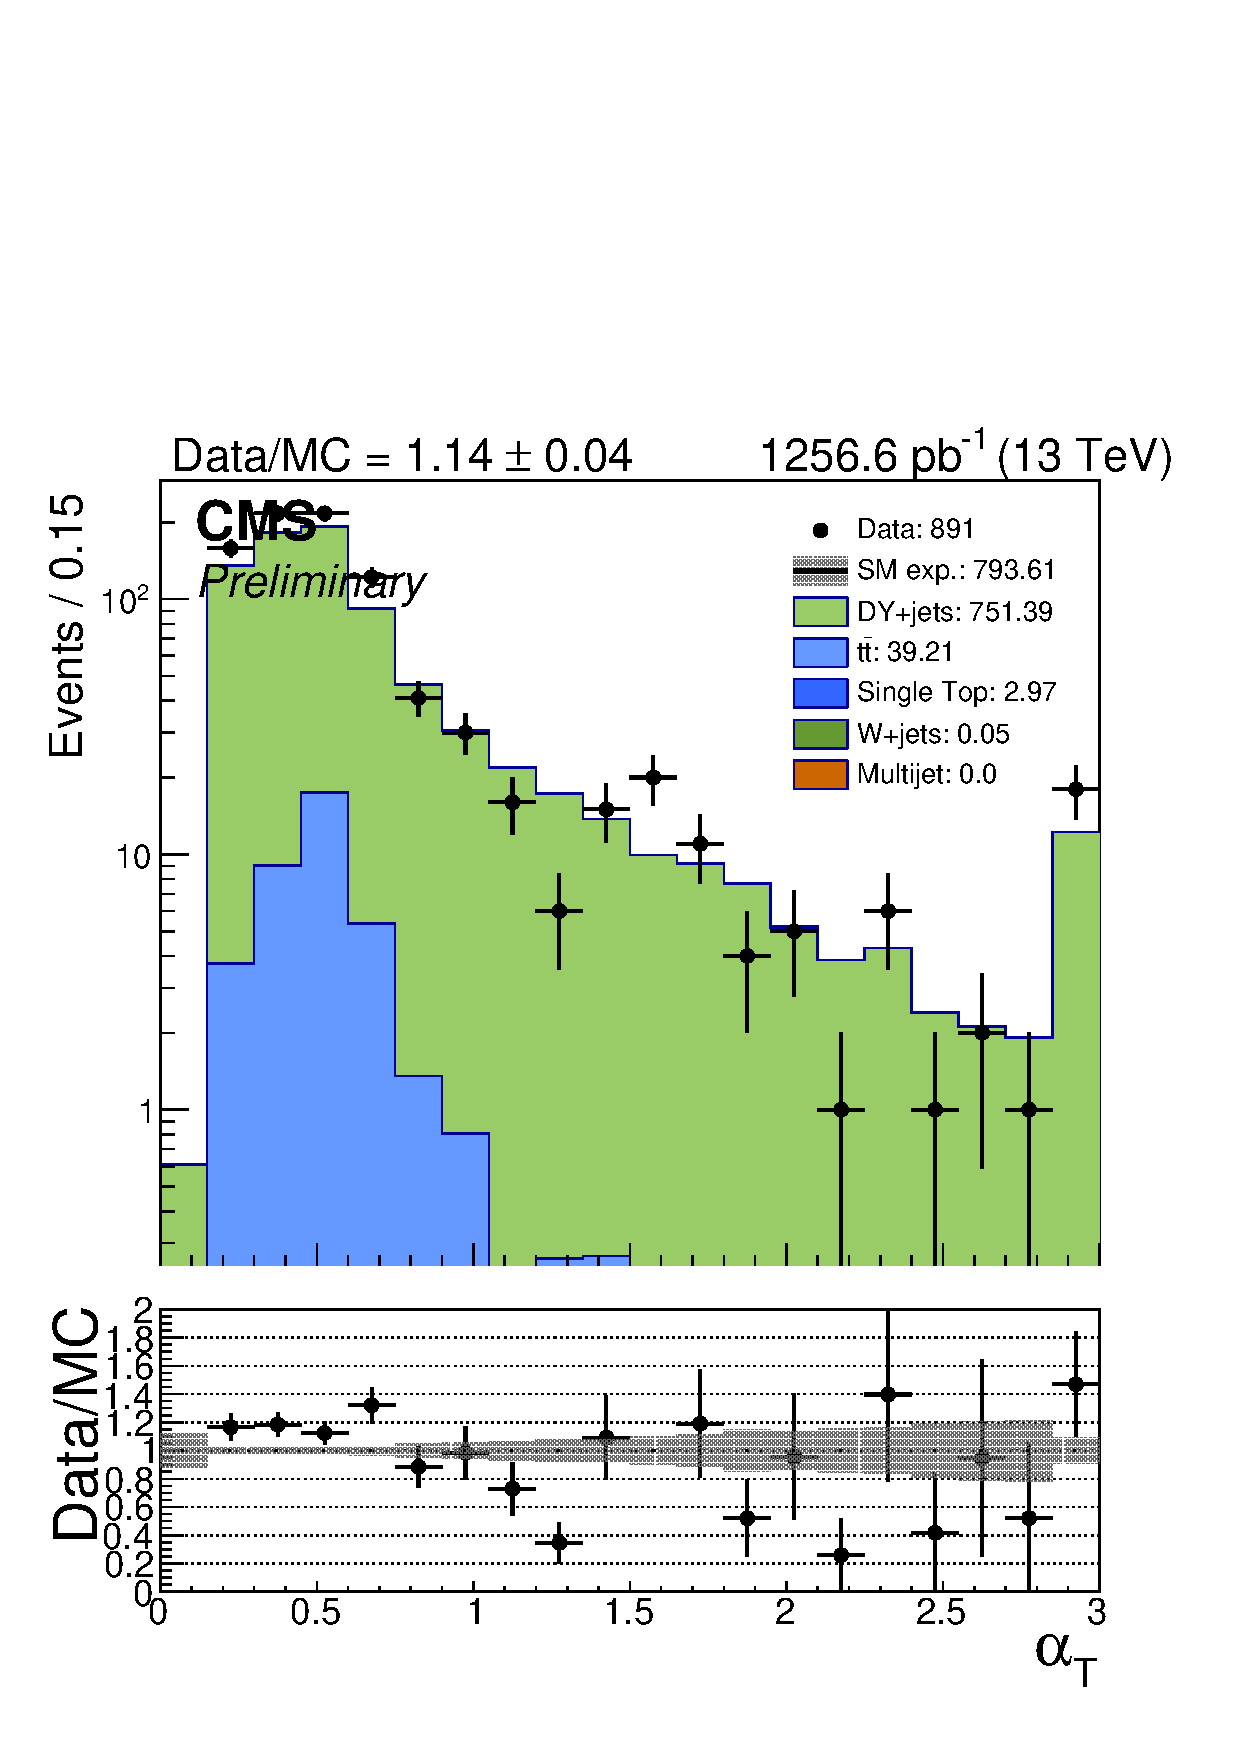
\includegraphics[width=0.5\textwidth]{figures/distributions/DoubleMu/alphaT_asym.pdf}} ~~
        \subfigure {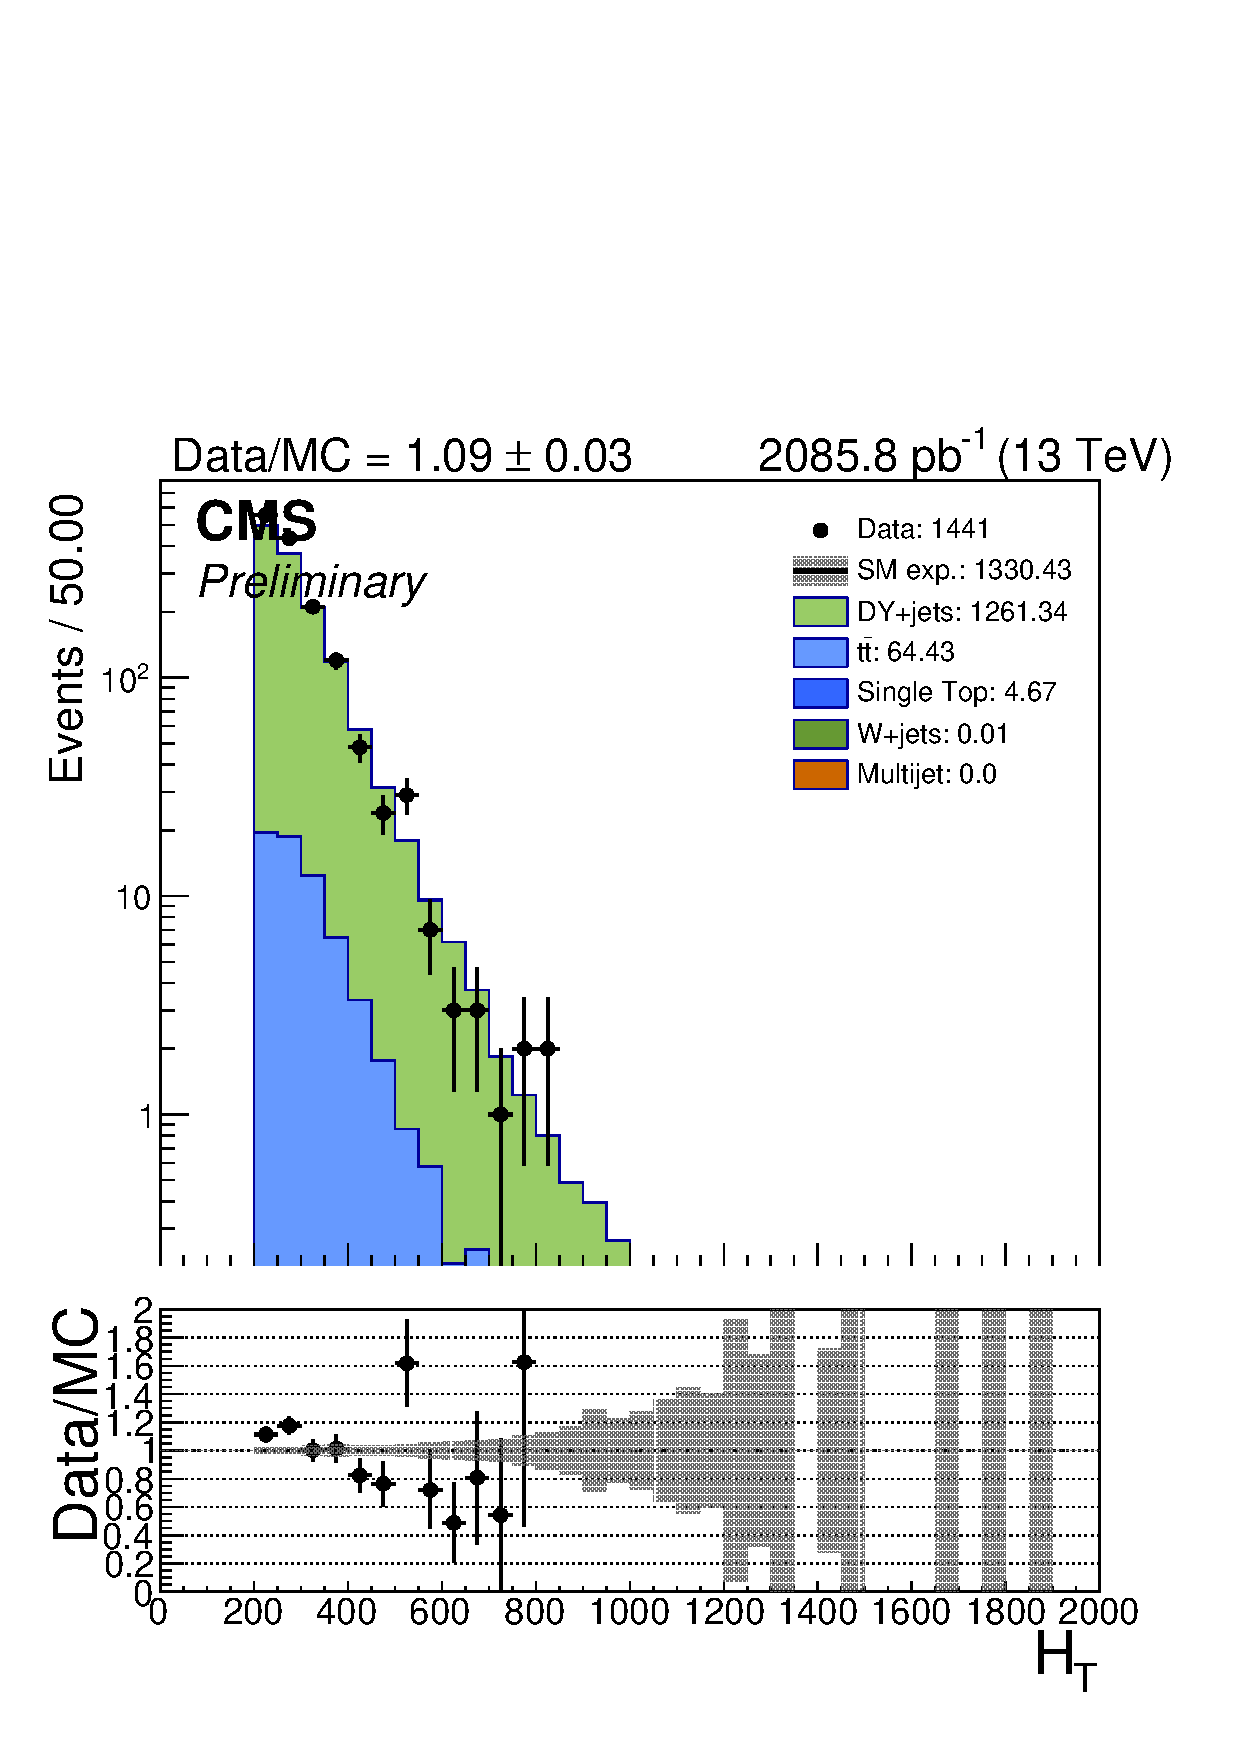
\includegraphics[width=0.5\textwidth]{figures/distributions/DoubleMu/ht40_asym.pdf}} \\
        \subfigure {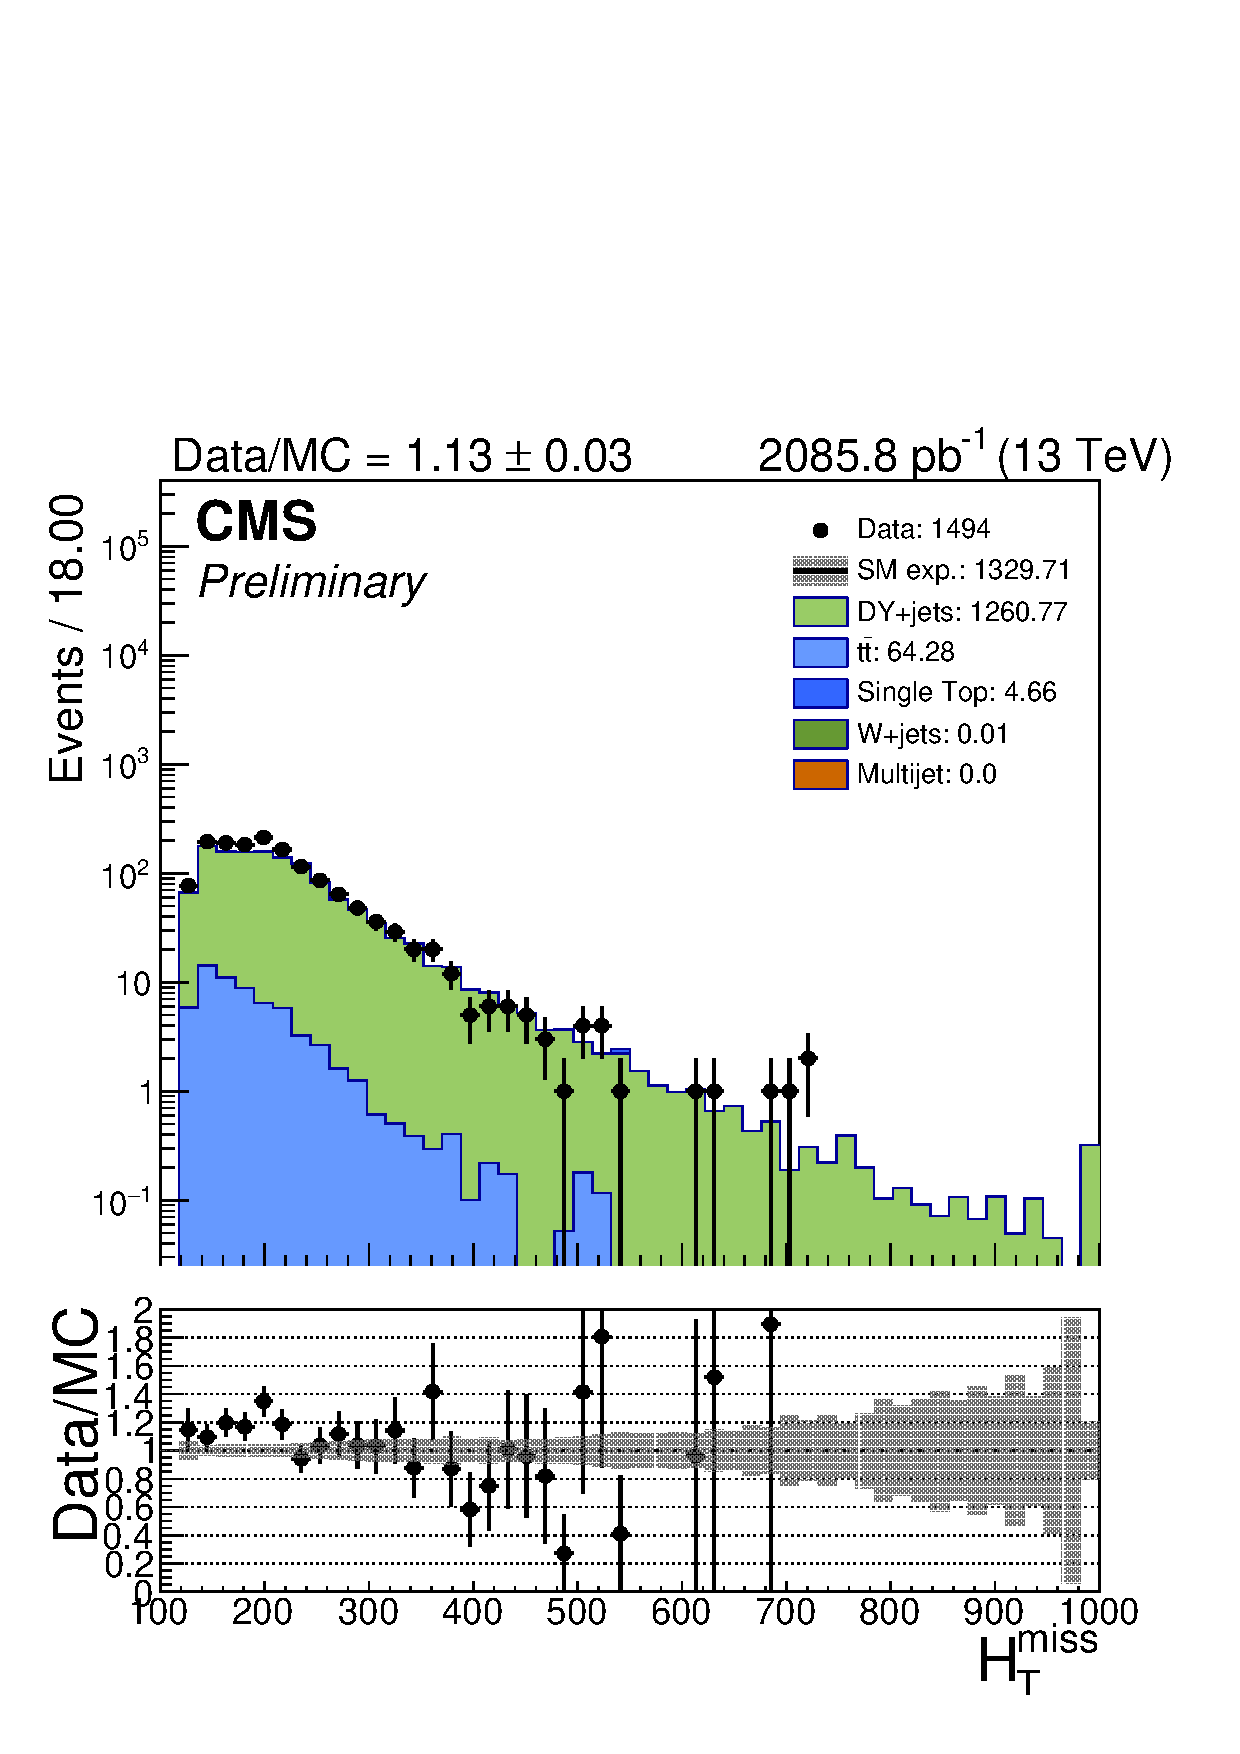
\includegraphics[width=0.5\textwidth]{figures/distributions/DoubleMu/mht40_pt_asym.pdf}} ~~
        \subfigure {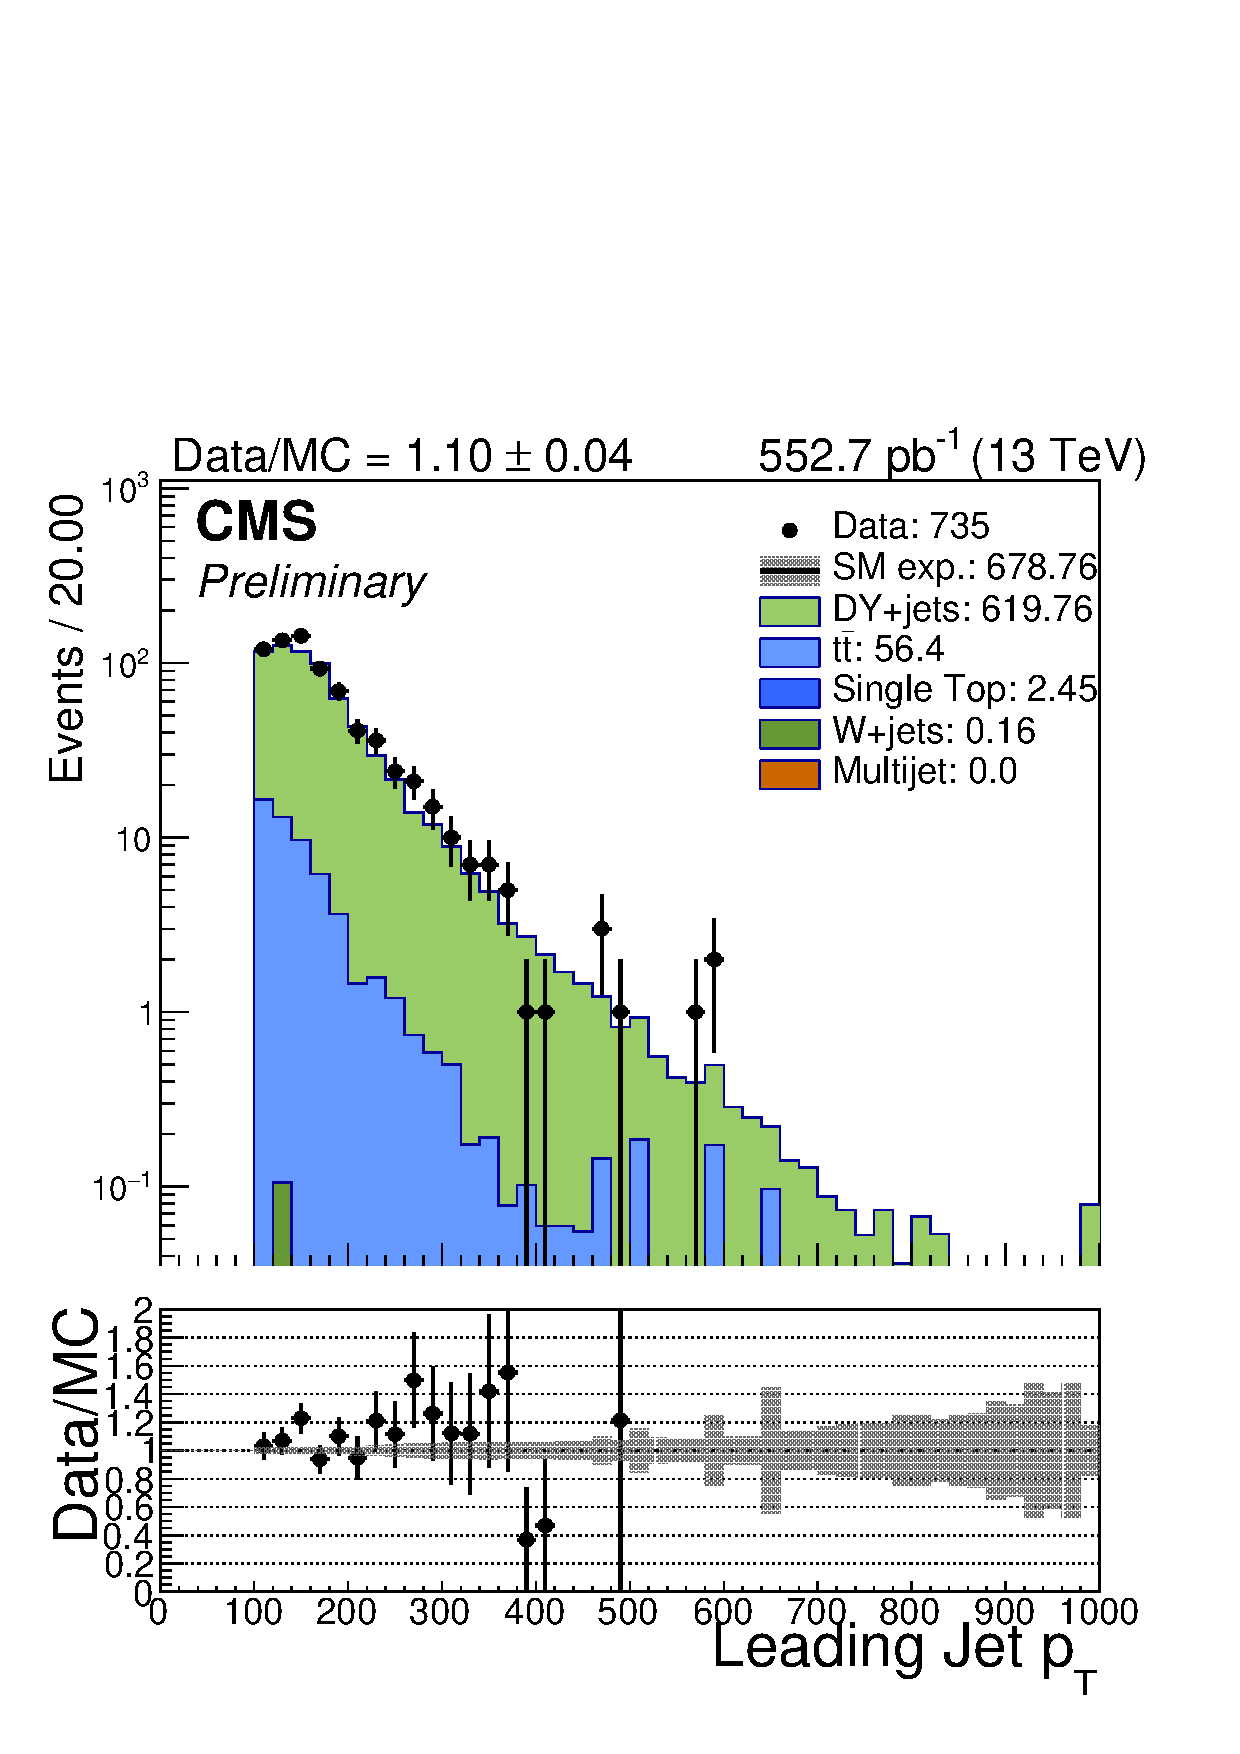
\includegraphics[width=0.5\textwidth]{figures/distributions/DoubleMu/jet_pt[0]_asym.pdf}} \\
        \caption{Key analysis variables for double muon control region (asymmetric bins)}
        \label{fig:distribution_doublemu_asym}
    \end{center}
\end{figure}

\begin{figure}
    \begin{center} 
        \subfigure {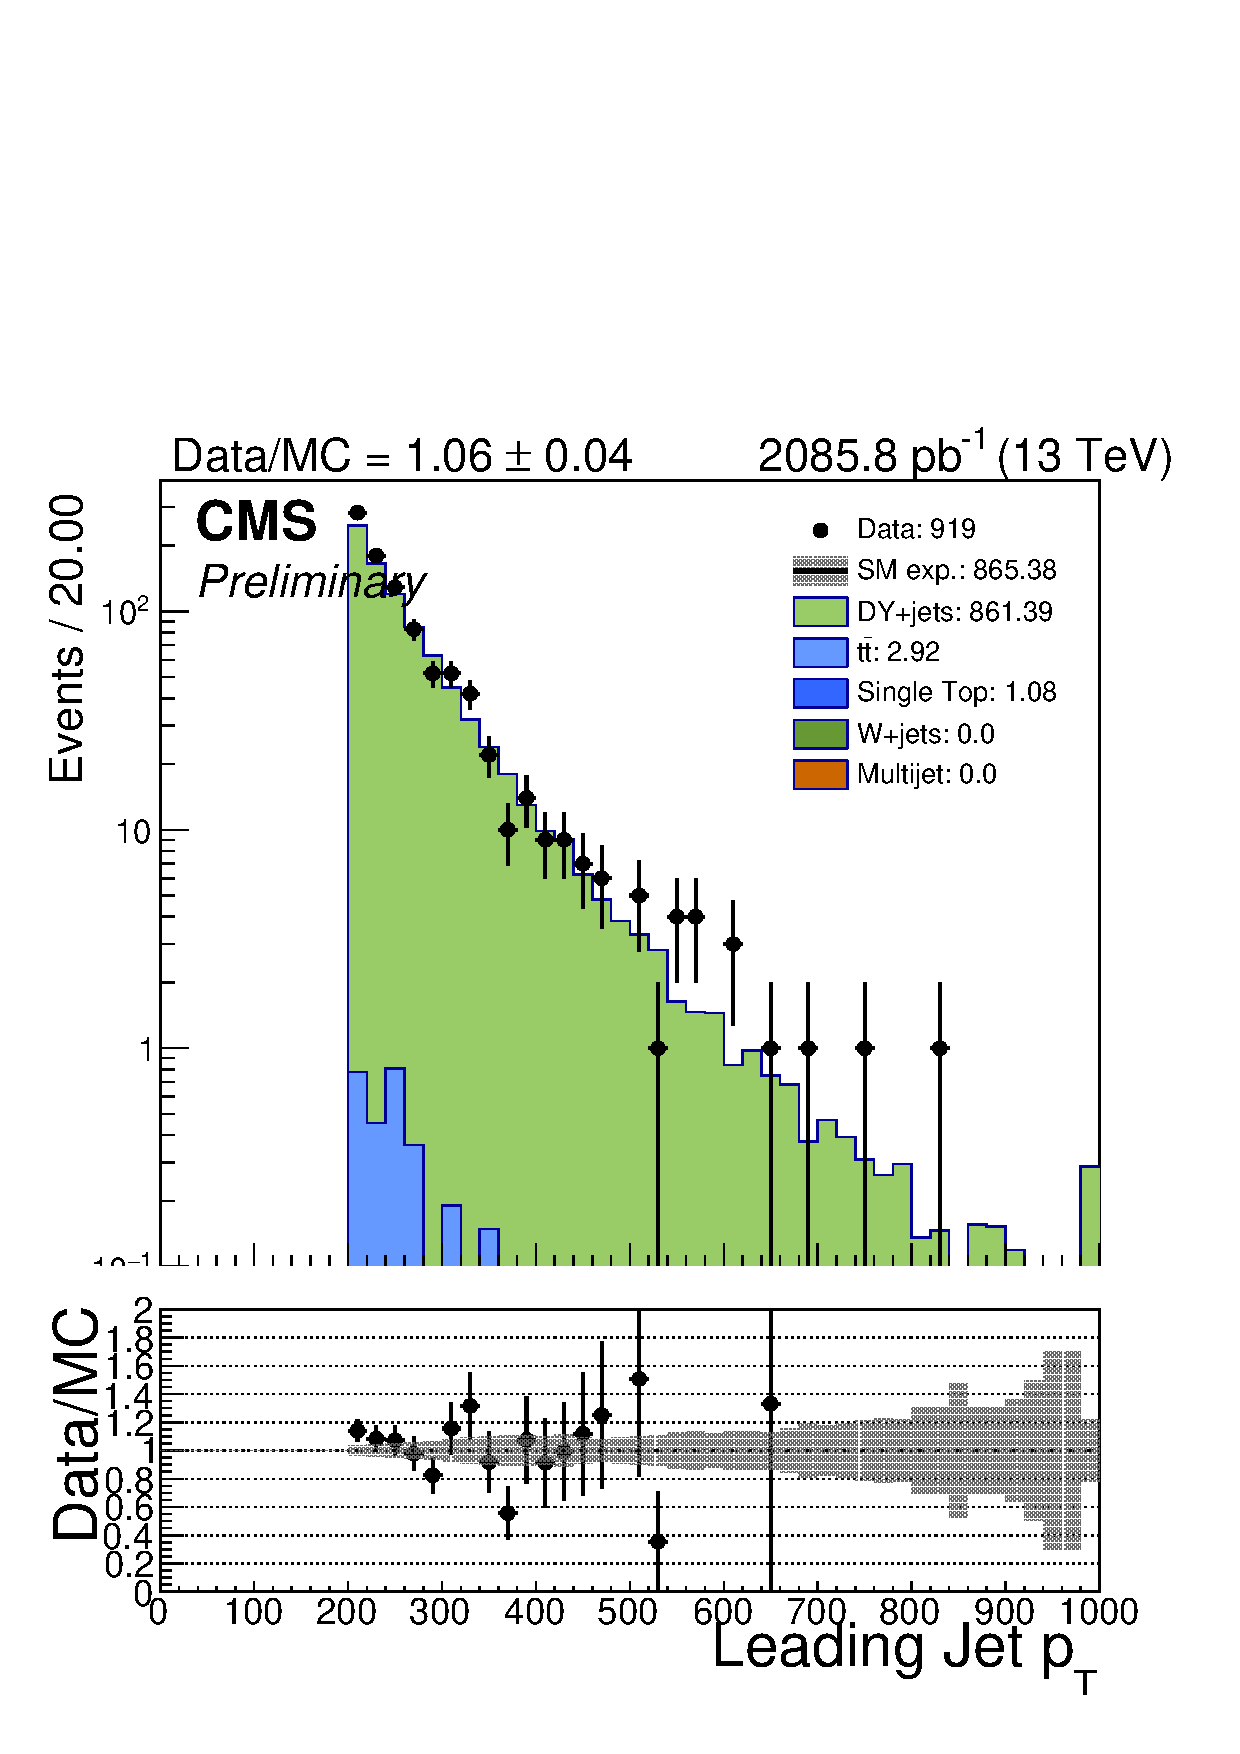
\includegraphics[width=0.5\textwidth]{figures/distributions/DoubleMu/jet_pt[0]_eq1j.pdf}} ~~
        \subfigure {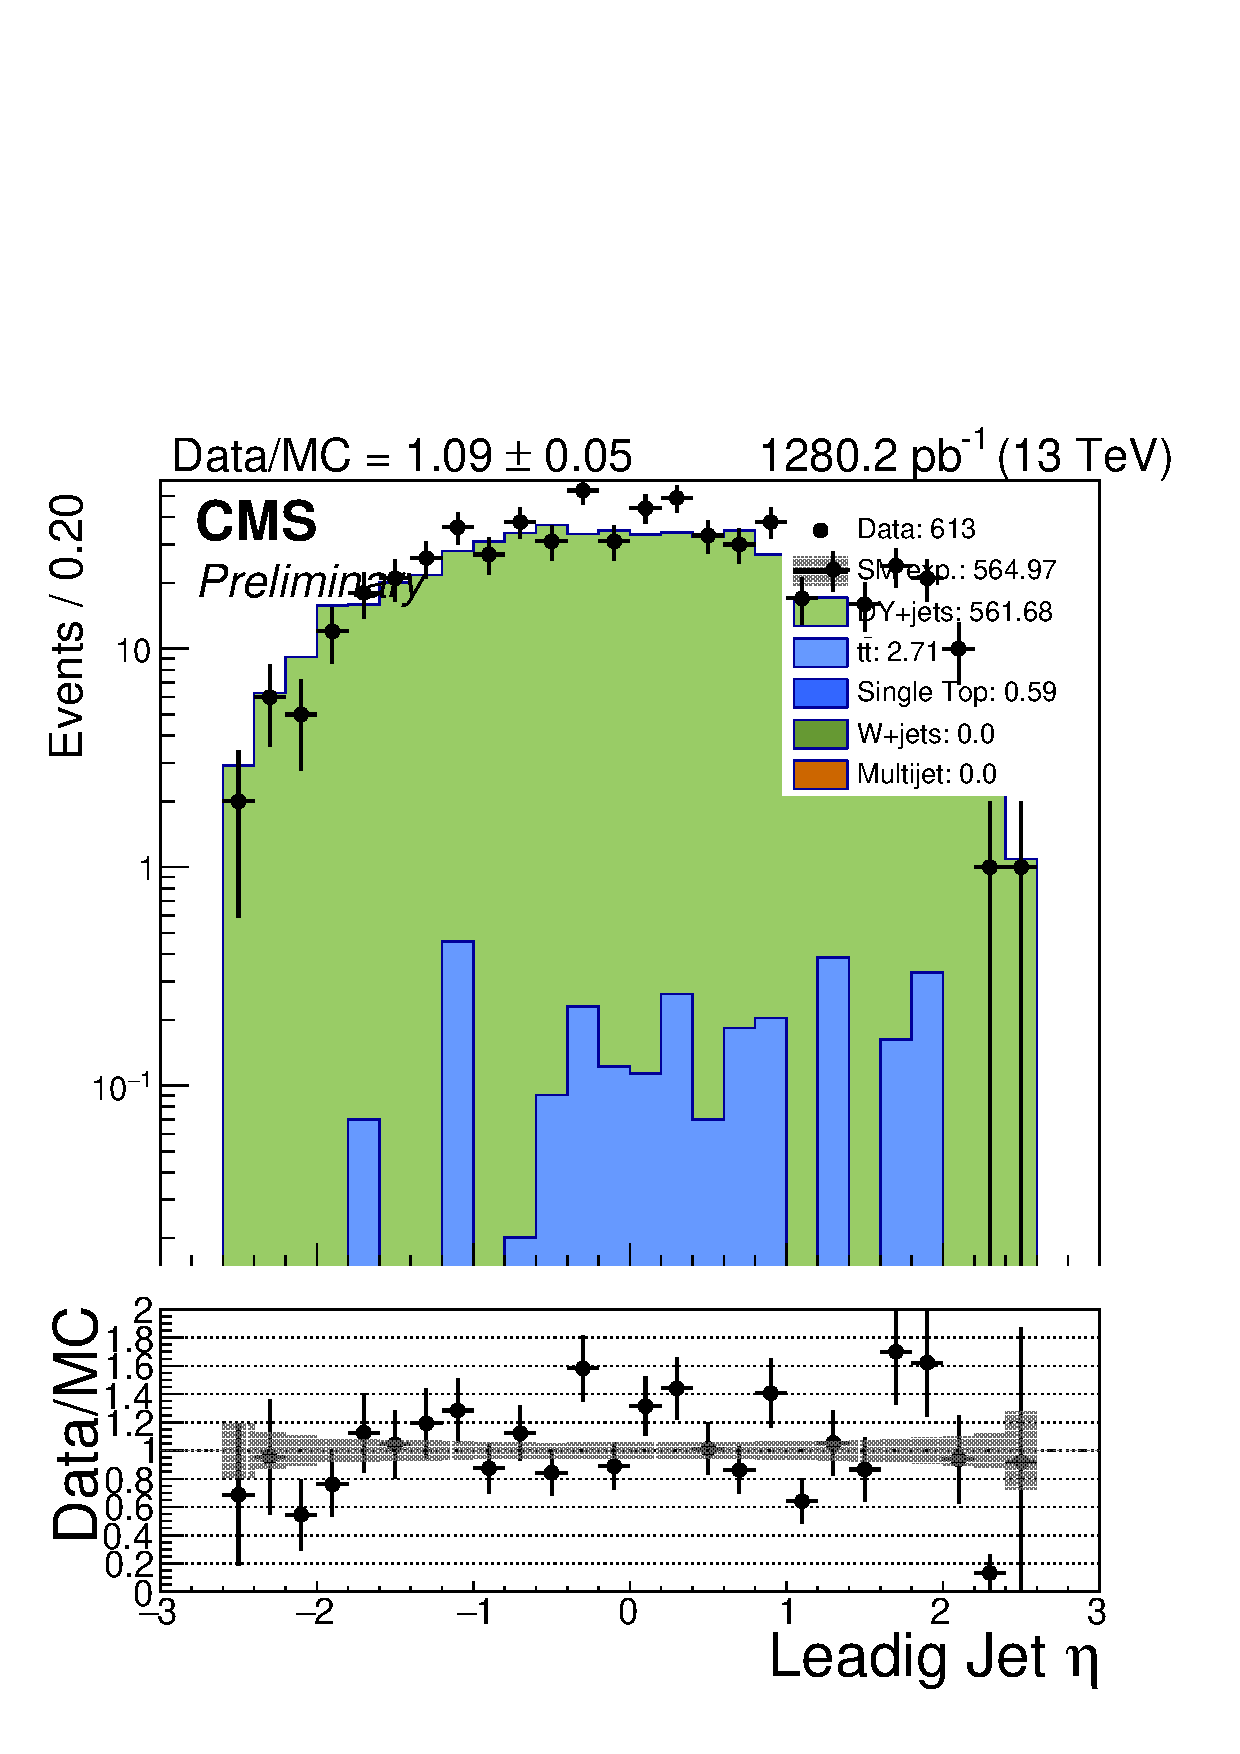
\includegraphics[width=0.5\textwidth]{figures/distributions/DoubleMu/jet_eta[0]_eq1j.pdf}} \\
        \subfigure {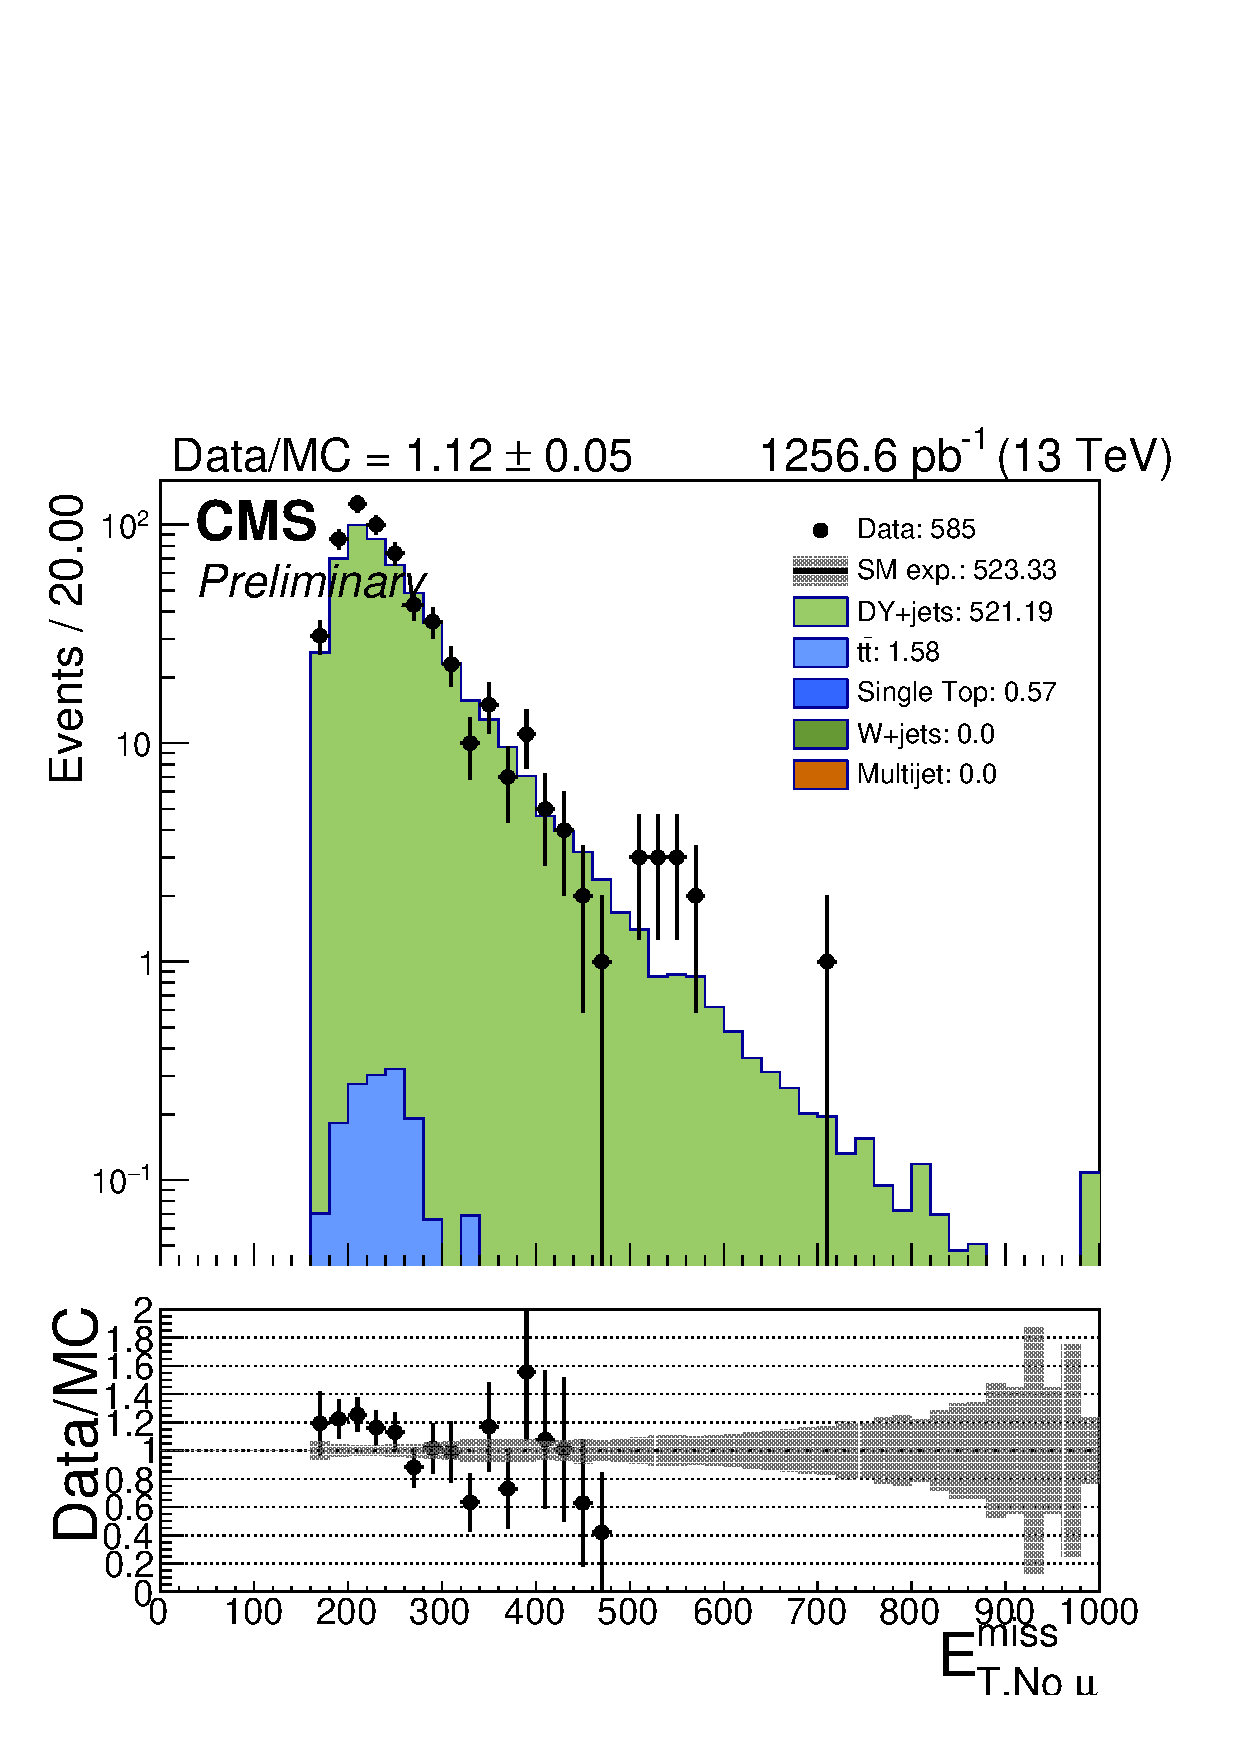
\includegraphics[width=0.5\textwidth]{figures/distributions/DoubleMu/metNoMu_pt_eq1j.pdf}} ~~
        \subfigure {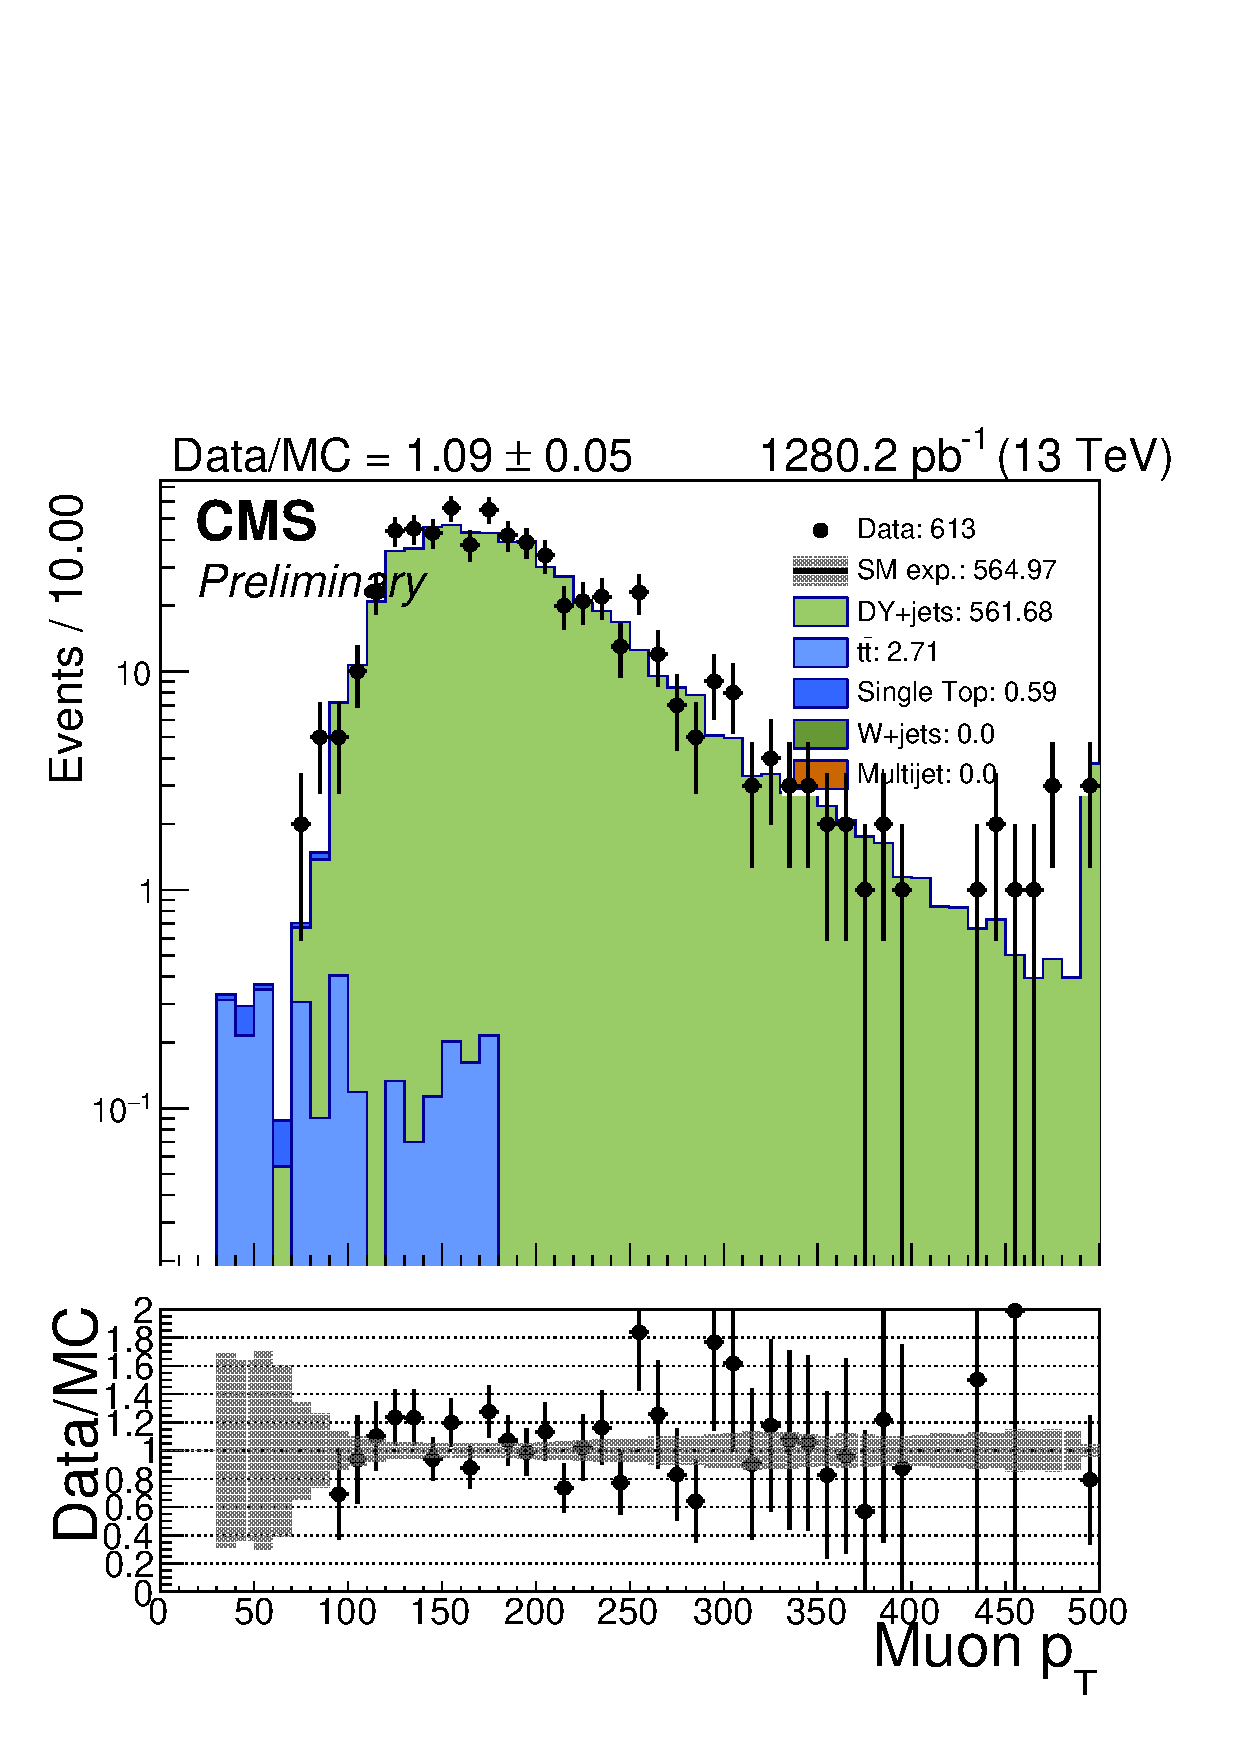
\includegraphics[width=0.5\textwidth]{figures/distributions/DoubleMu/muon_pt[0]_eq1j.pdf}} \\
        \caption{Key analysis variables for double muon control region (monojet bins)}
        \label{fig:distribution_doublemu_mono}
    \end{center}
\end{figure}
%%____________________________________________________________________________||
\begin{figure}
    \begin{center}
        \subfigure {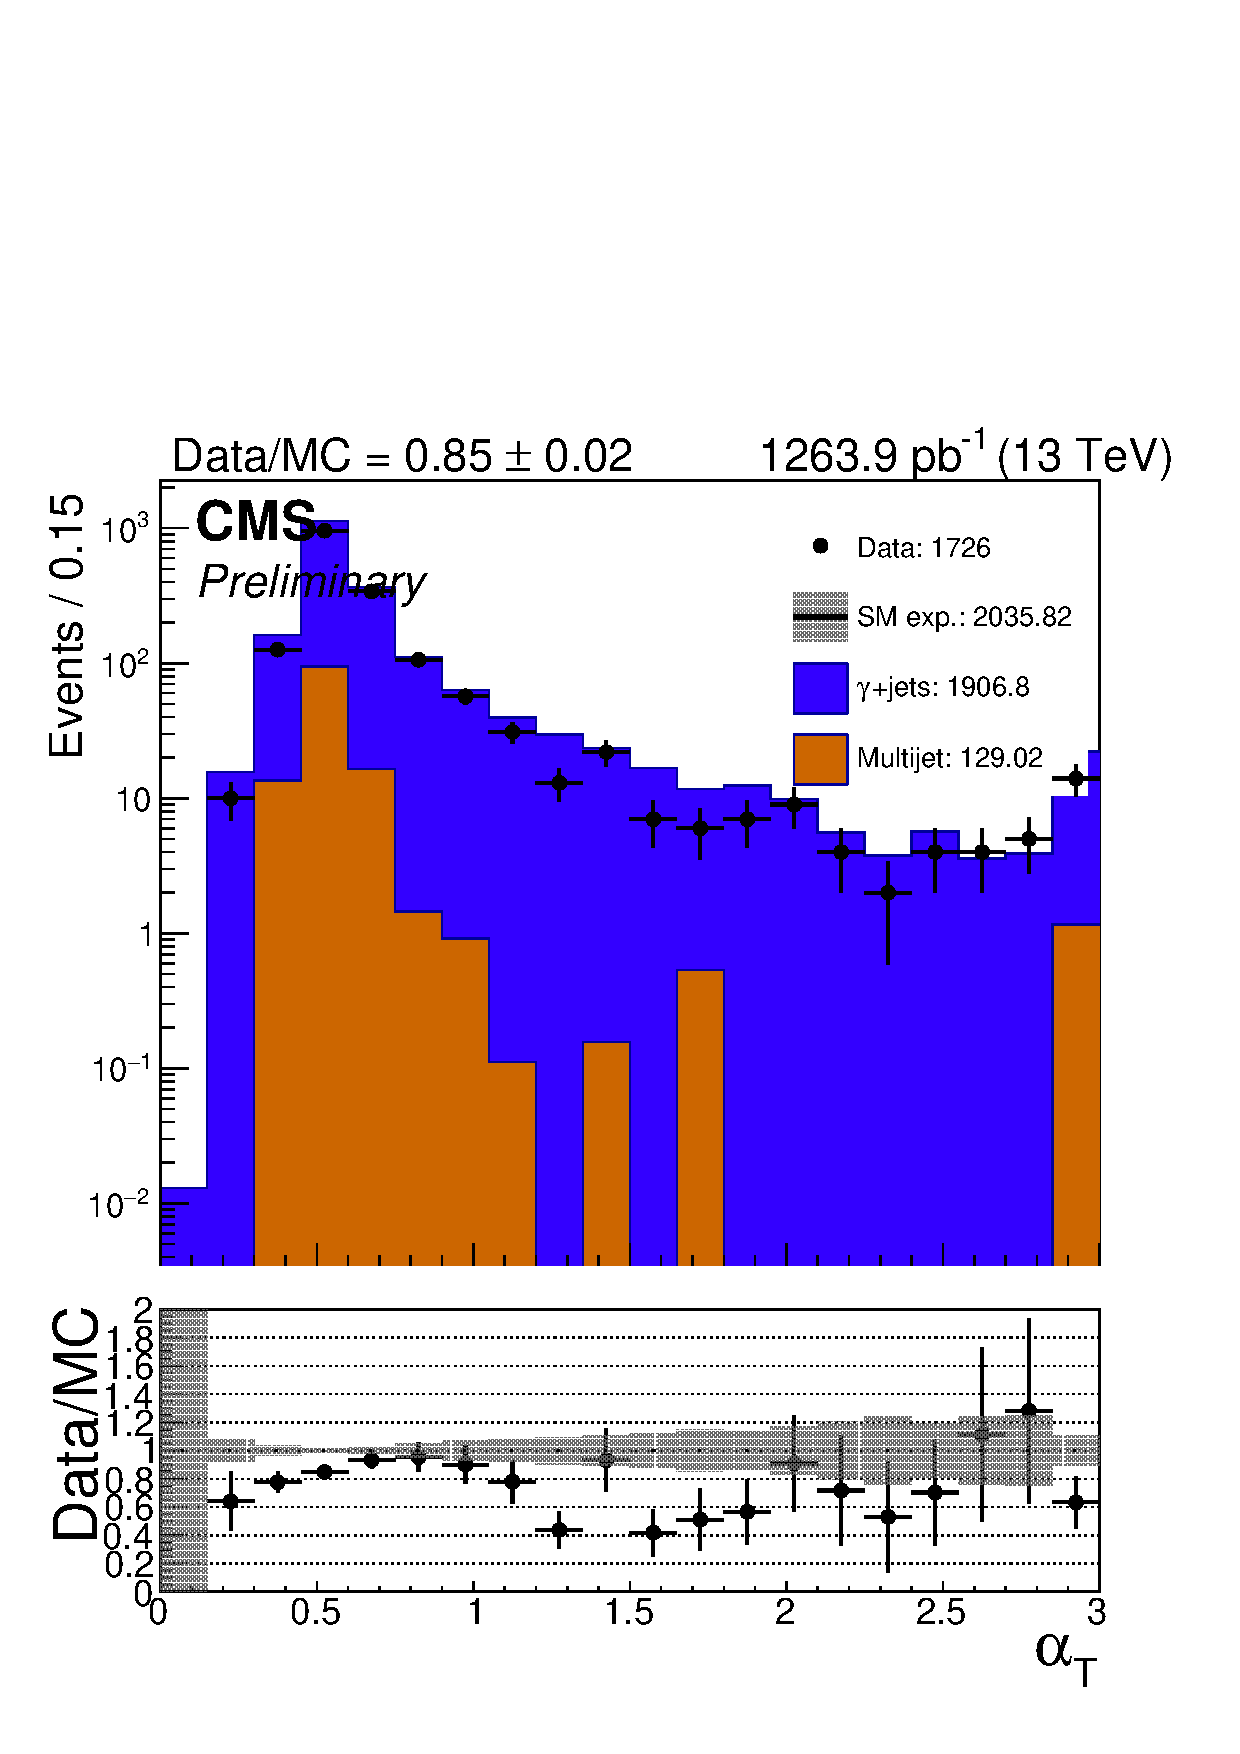
\includegraphics[width=0.5\textwidth]{figures/distributions/SinglePhoton/alphaT_sym.pdf}} ~~
        \subfigure {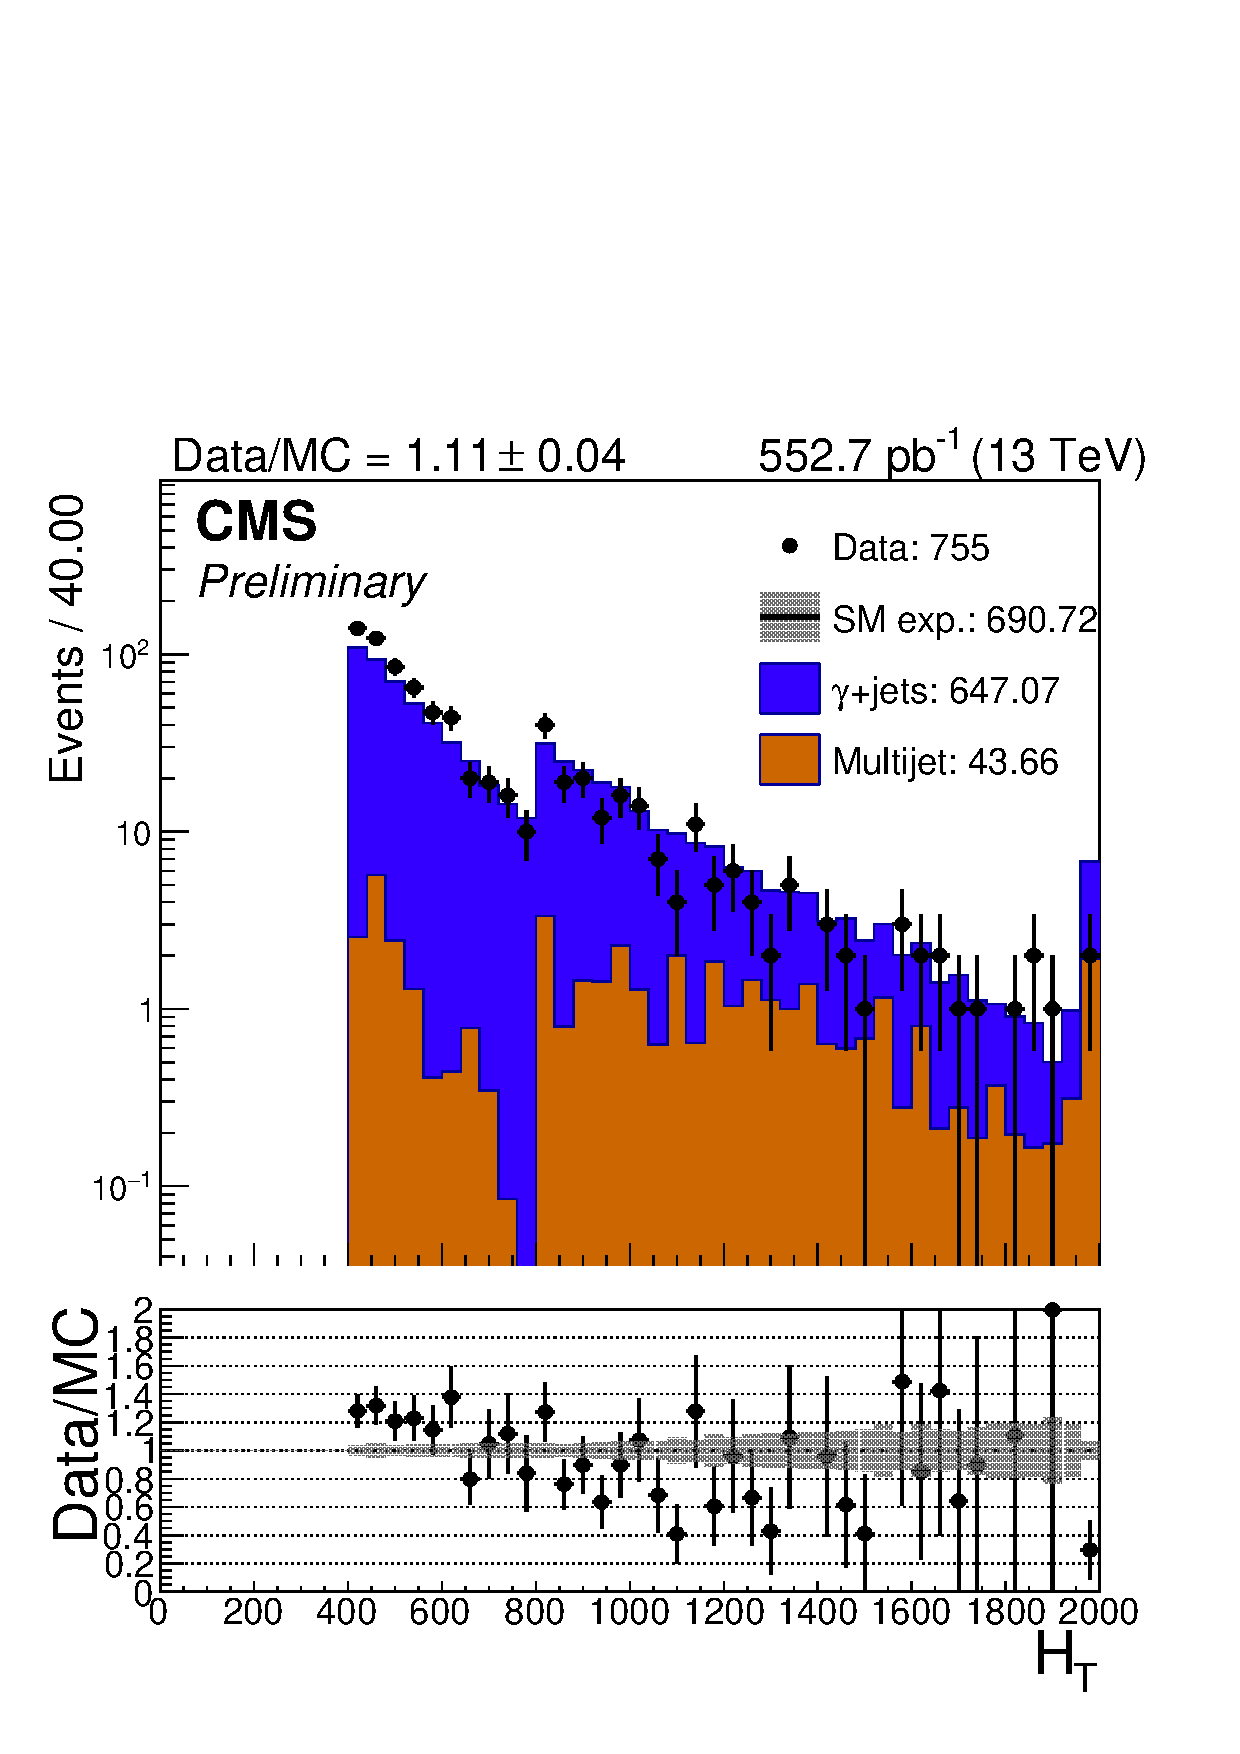
\includegraphics[width=0.5\textwidth]{figures/distributions/SinglePhoton/ht40_sym.pdf}} \\
        \subfigure {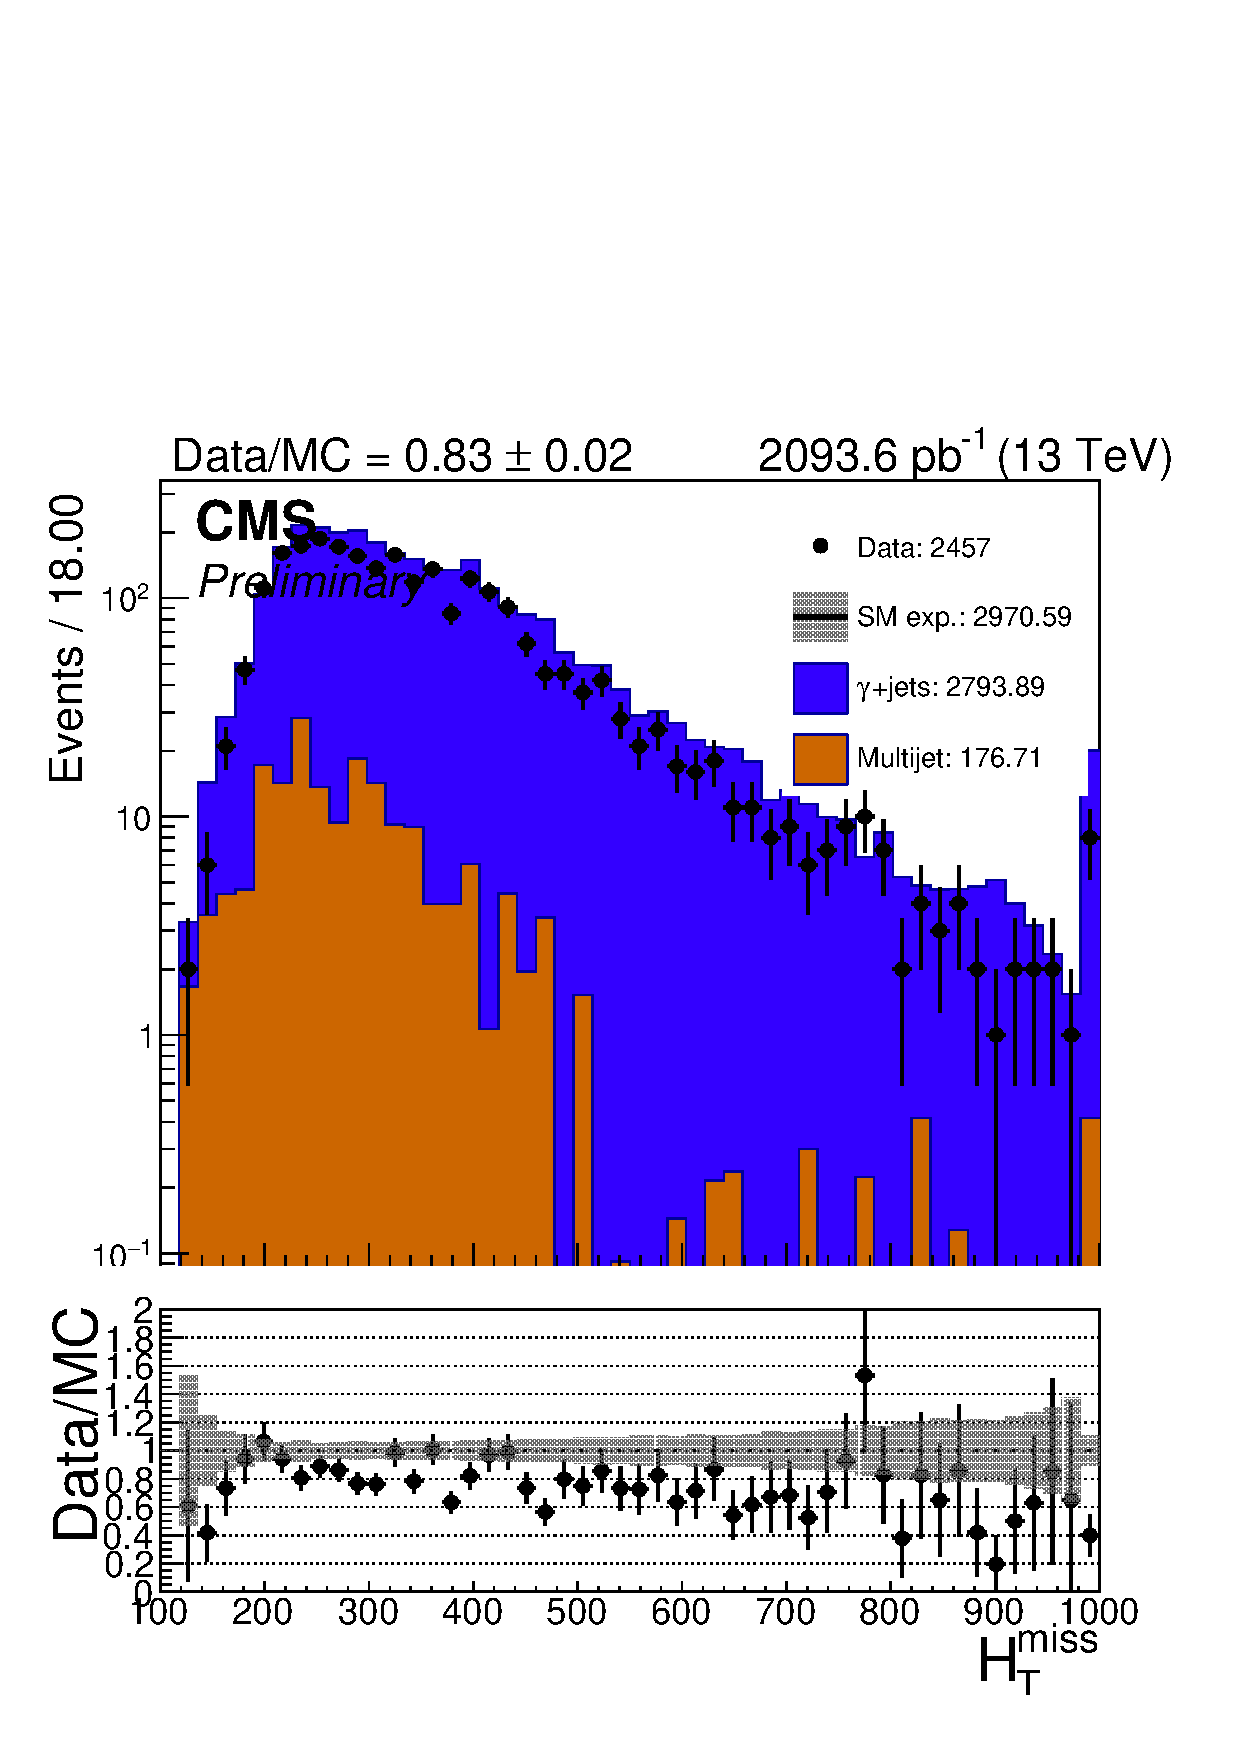
\includegraphics[width=0.5\textwidth]{figures/distributions/SinglePhoton/mht40_pt_sym.pdf}} ~~
        \subfigure {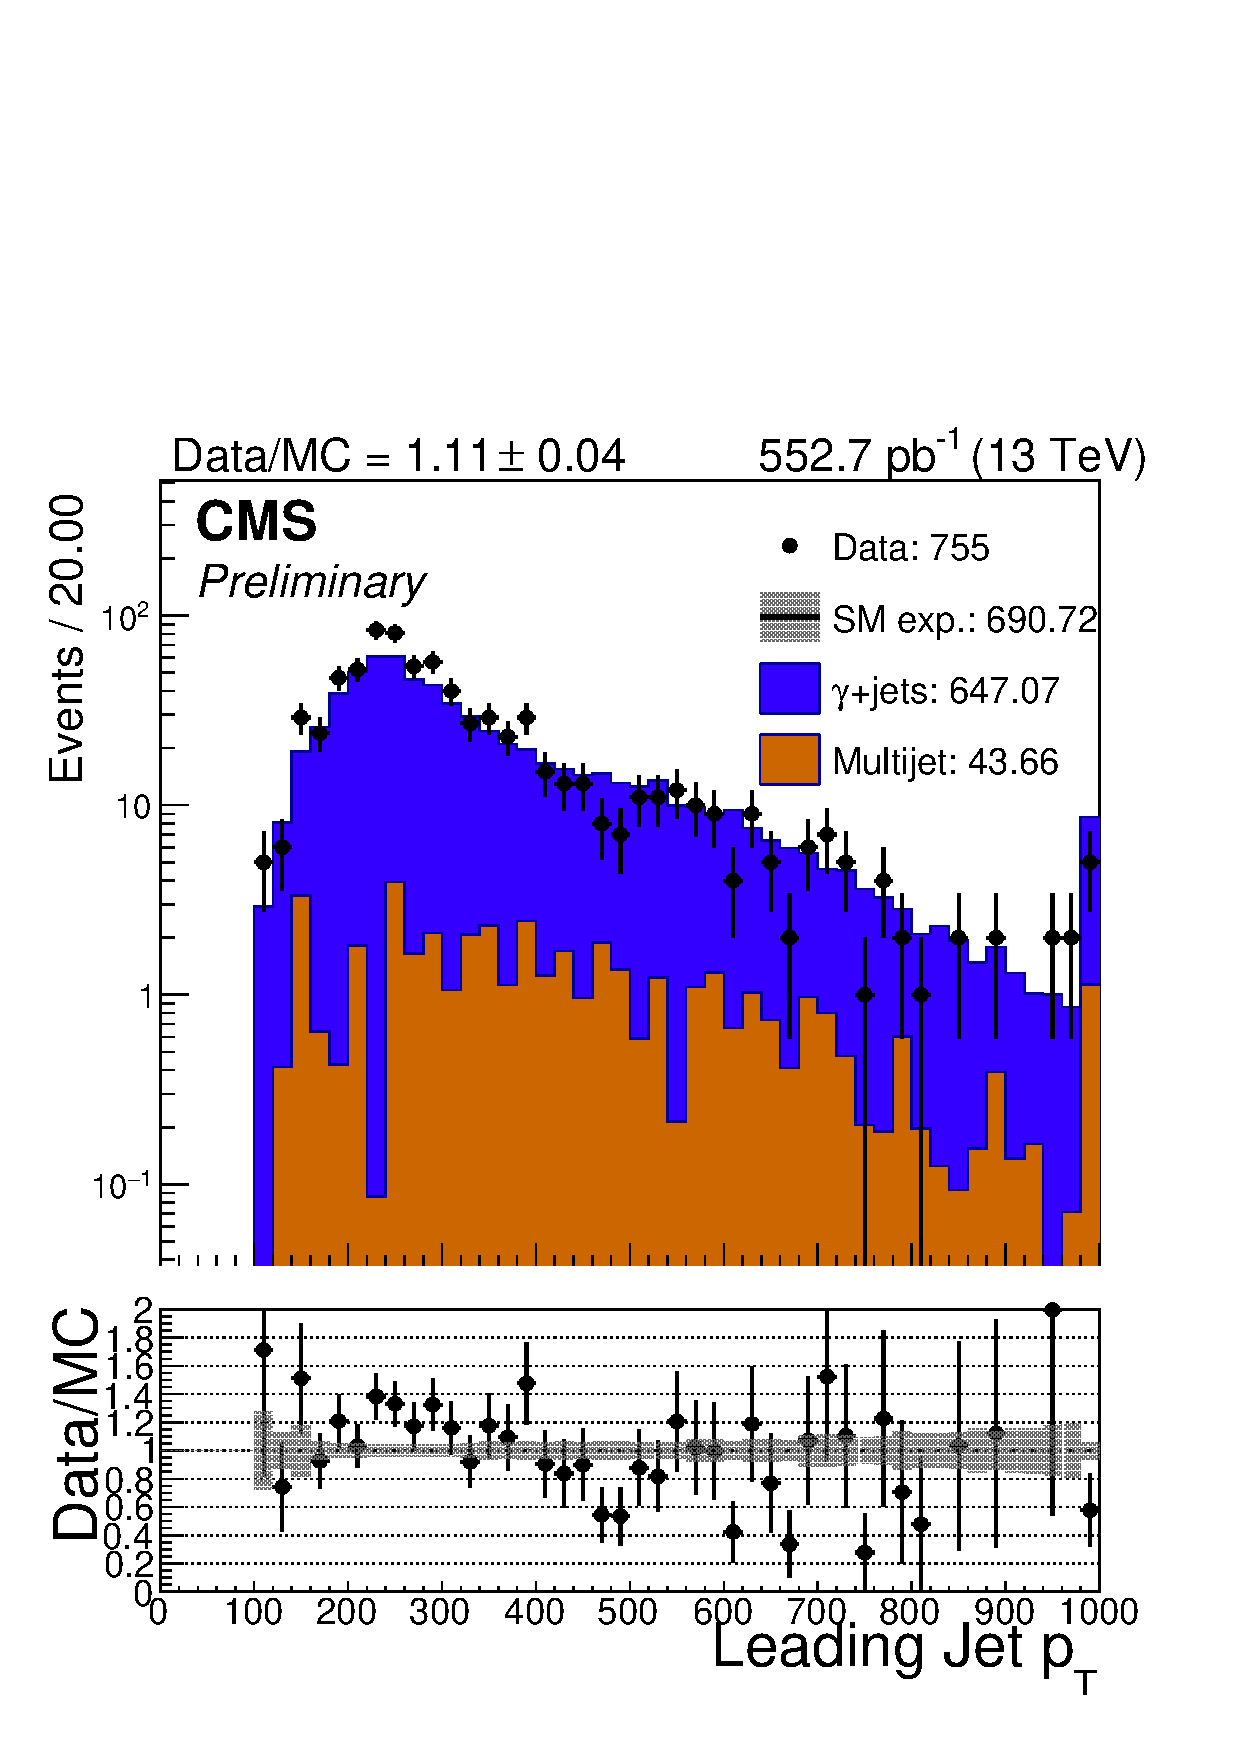
\includegraphics[width=0.5\textwidth]{figures/distributions/SinglePhoton/jet_pt[0]_sym.pdf}} \\
        \caption{Key analysis variables for single photon control region (symmetric bins)}
        \label{fig:distribution_singlephoton_sym}
    \end{center}
\end{figure}

\begin{figure}[h]
    \begin{center}
        \subfigure {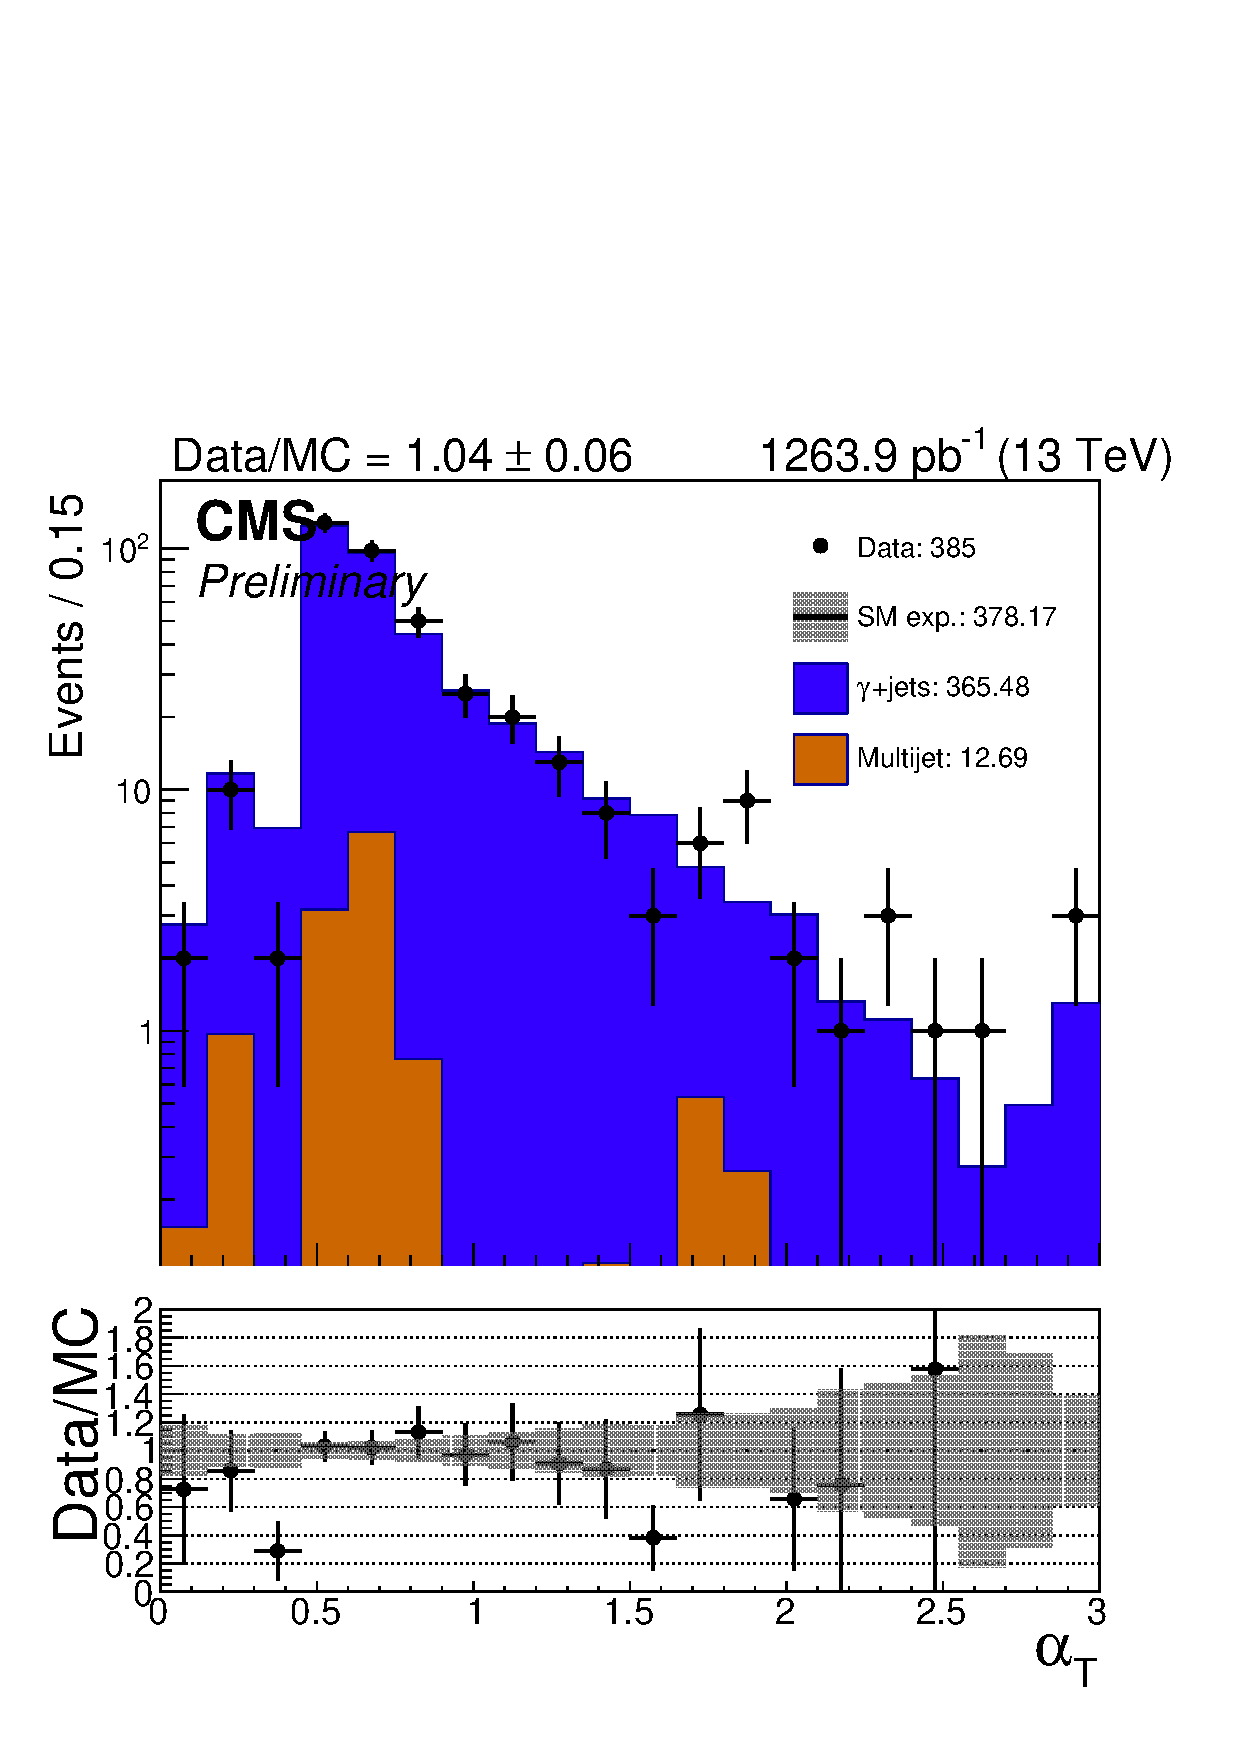
\includegraphics[width=0.5\textwidth]{figures/distributions/SinglePhoton/alphaT_asym.pdf}} ~~
        \subfigure {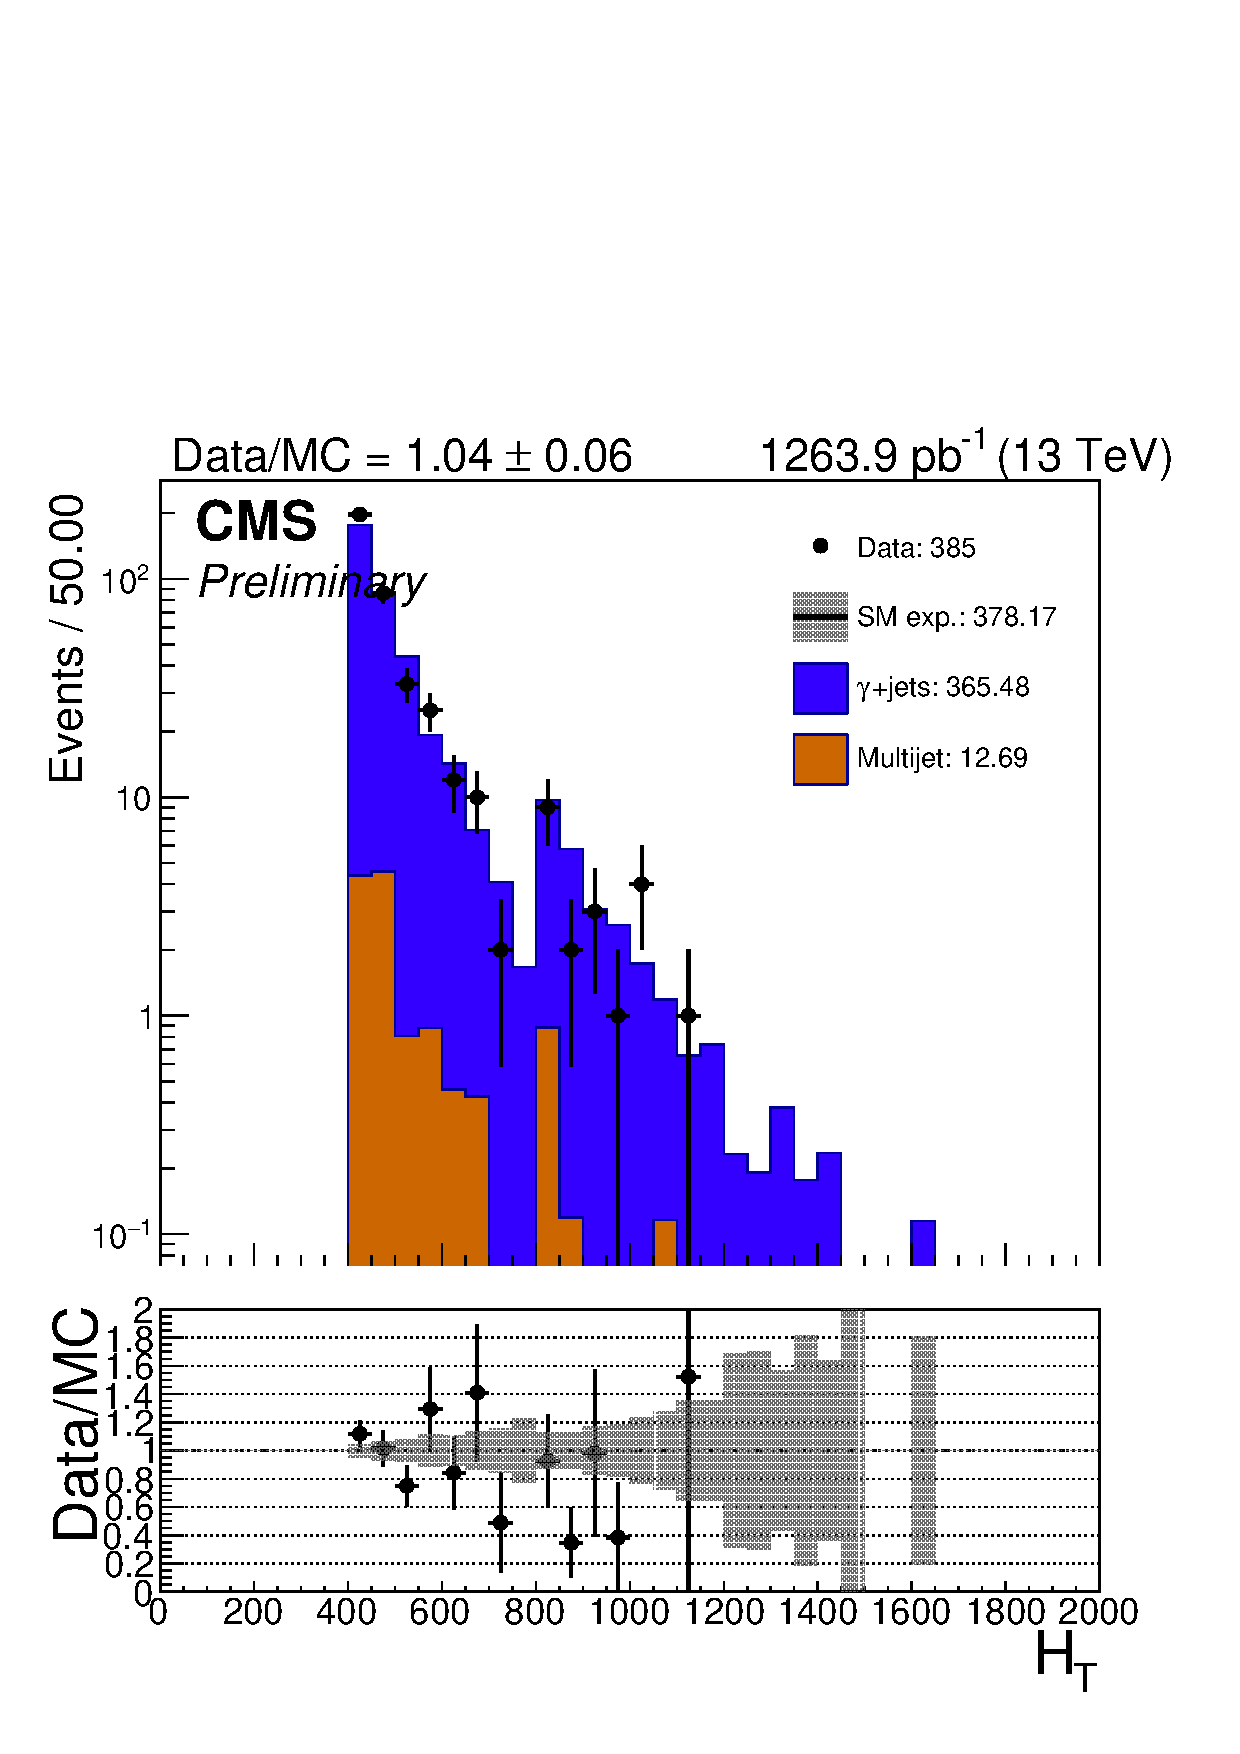
\includegraphics[width=0.5\textwidth]{figures/distributions/SinglePhoton/ht40_asym.pdf}} \\
        \subfigure {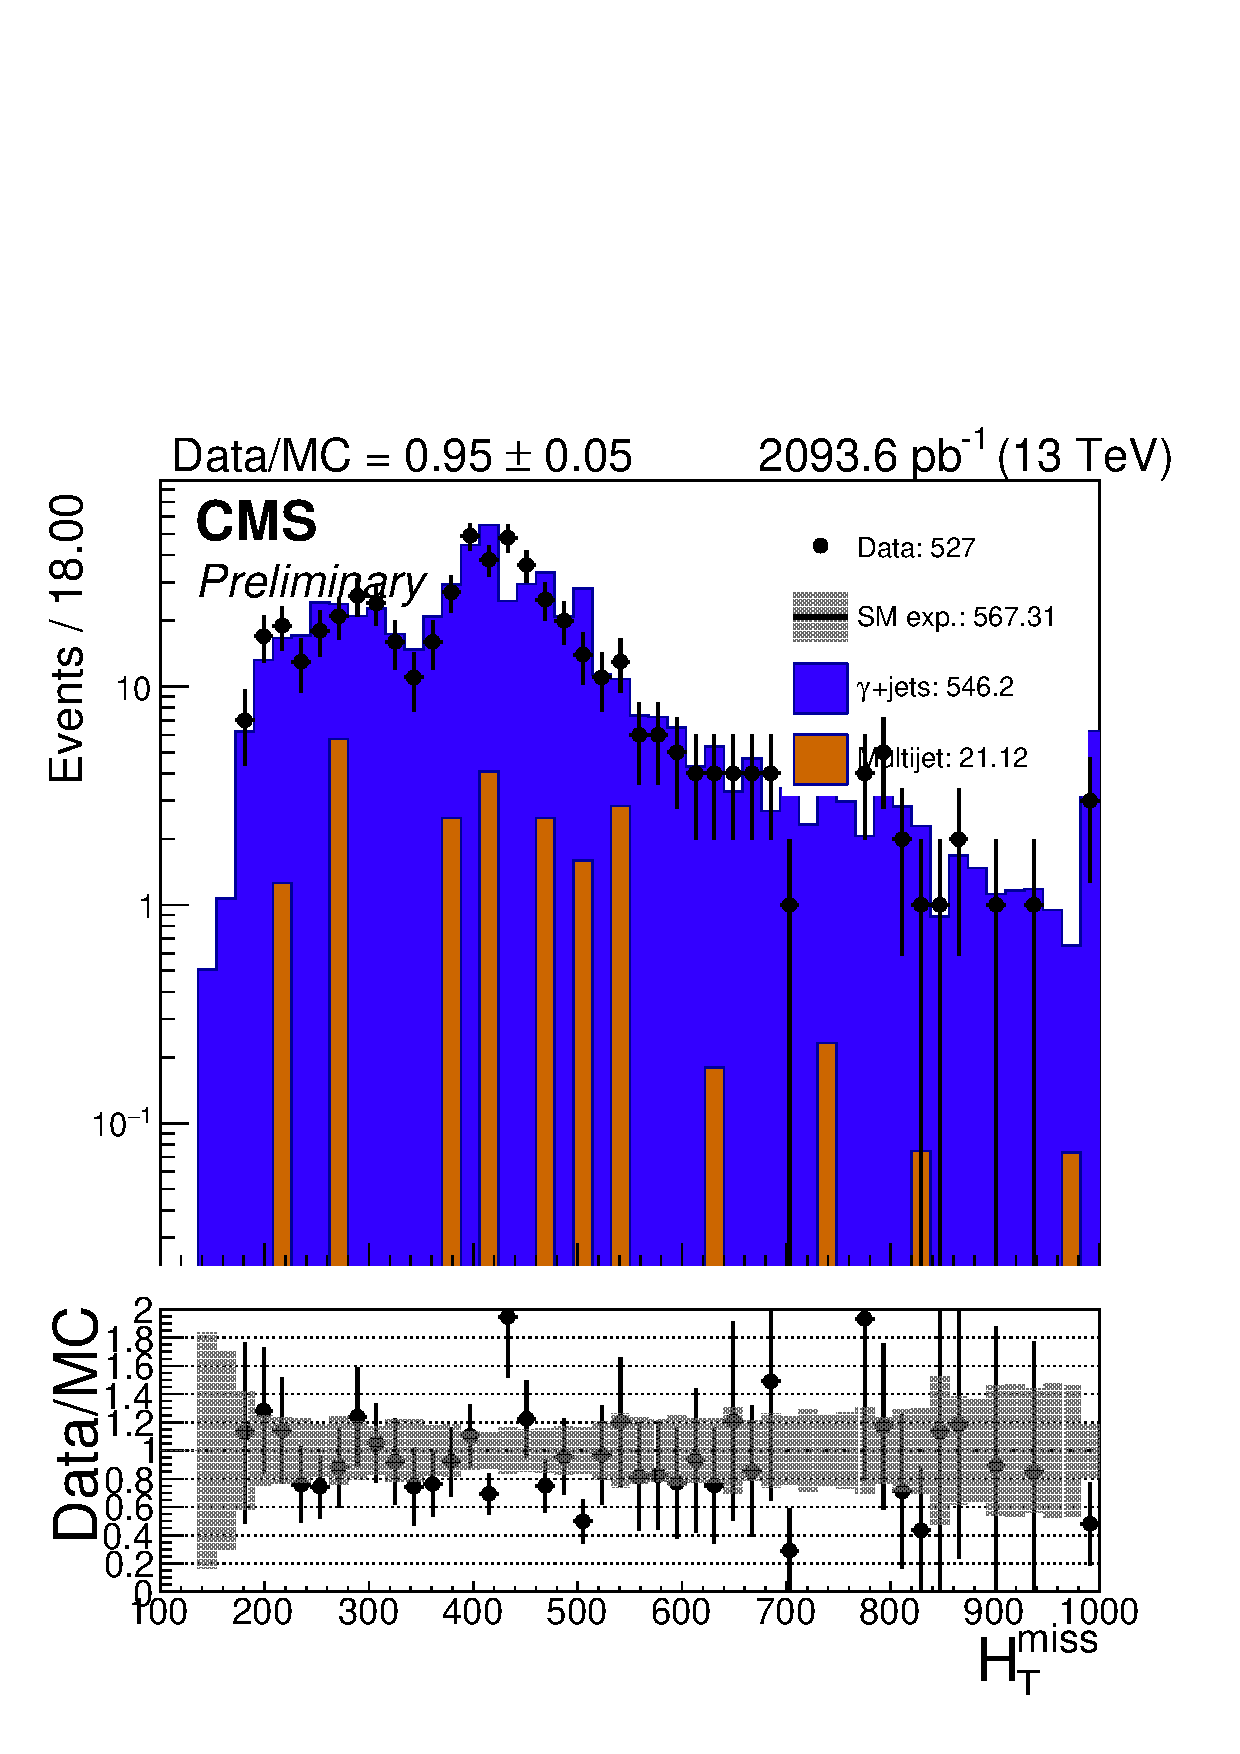
\includegraphics[width=0.5\textwidth]{figures/distributions/SinglePhoton/mht40_pt_asym.pdf}} ~~
        \subfigure {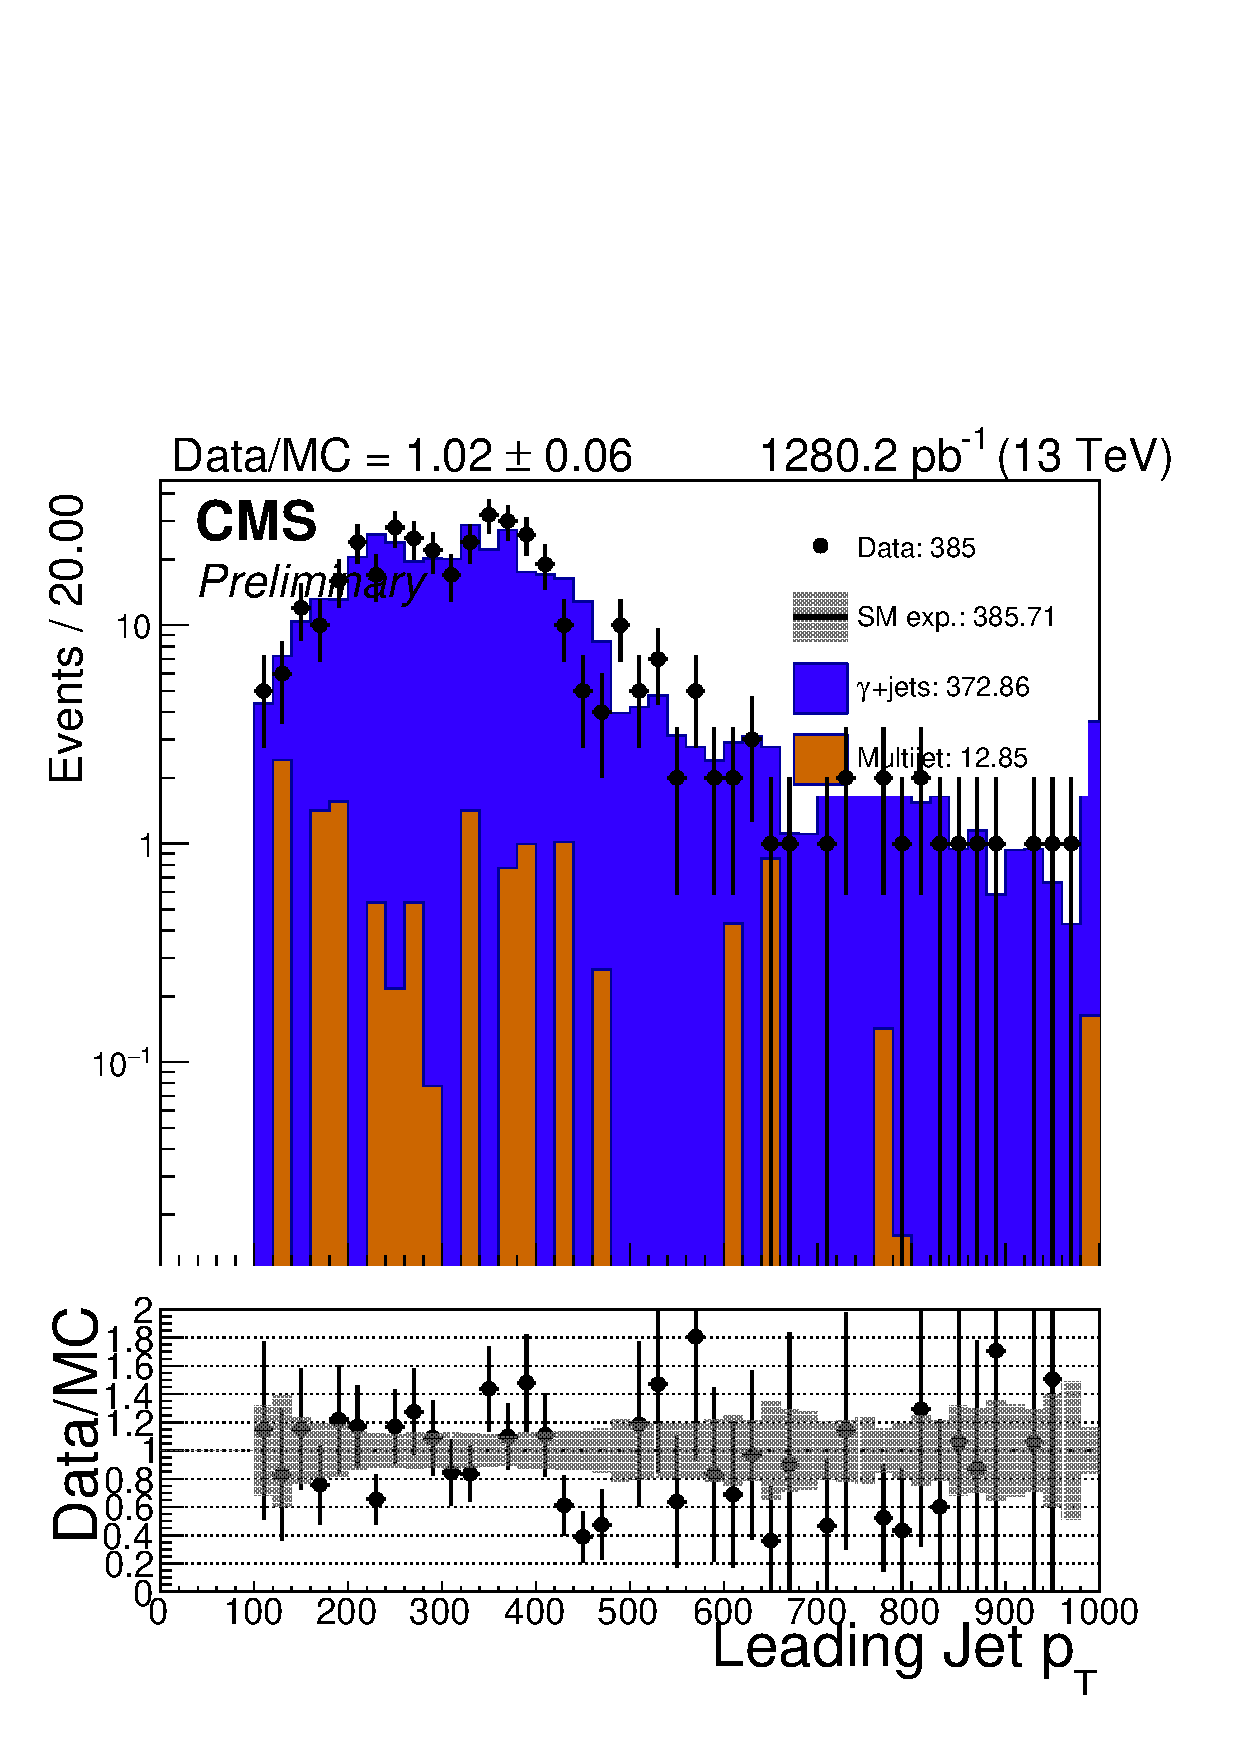
\includegraphics[width=0.5\textwidth]{figures/distributions/SinglePhoton/jet_pt[0]_asym.pdf}} \\
        \caption{Key analysis variables for single photon control region (asymmetric bins)}
        \label{fig:distribution_singlephoton_asym}
    \end{center}
\end{figure}

\begin{figure}
    \begin{center} 
        \subfigure {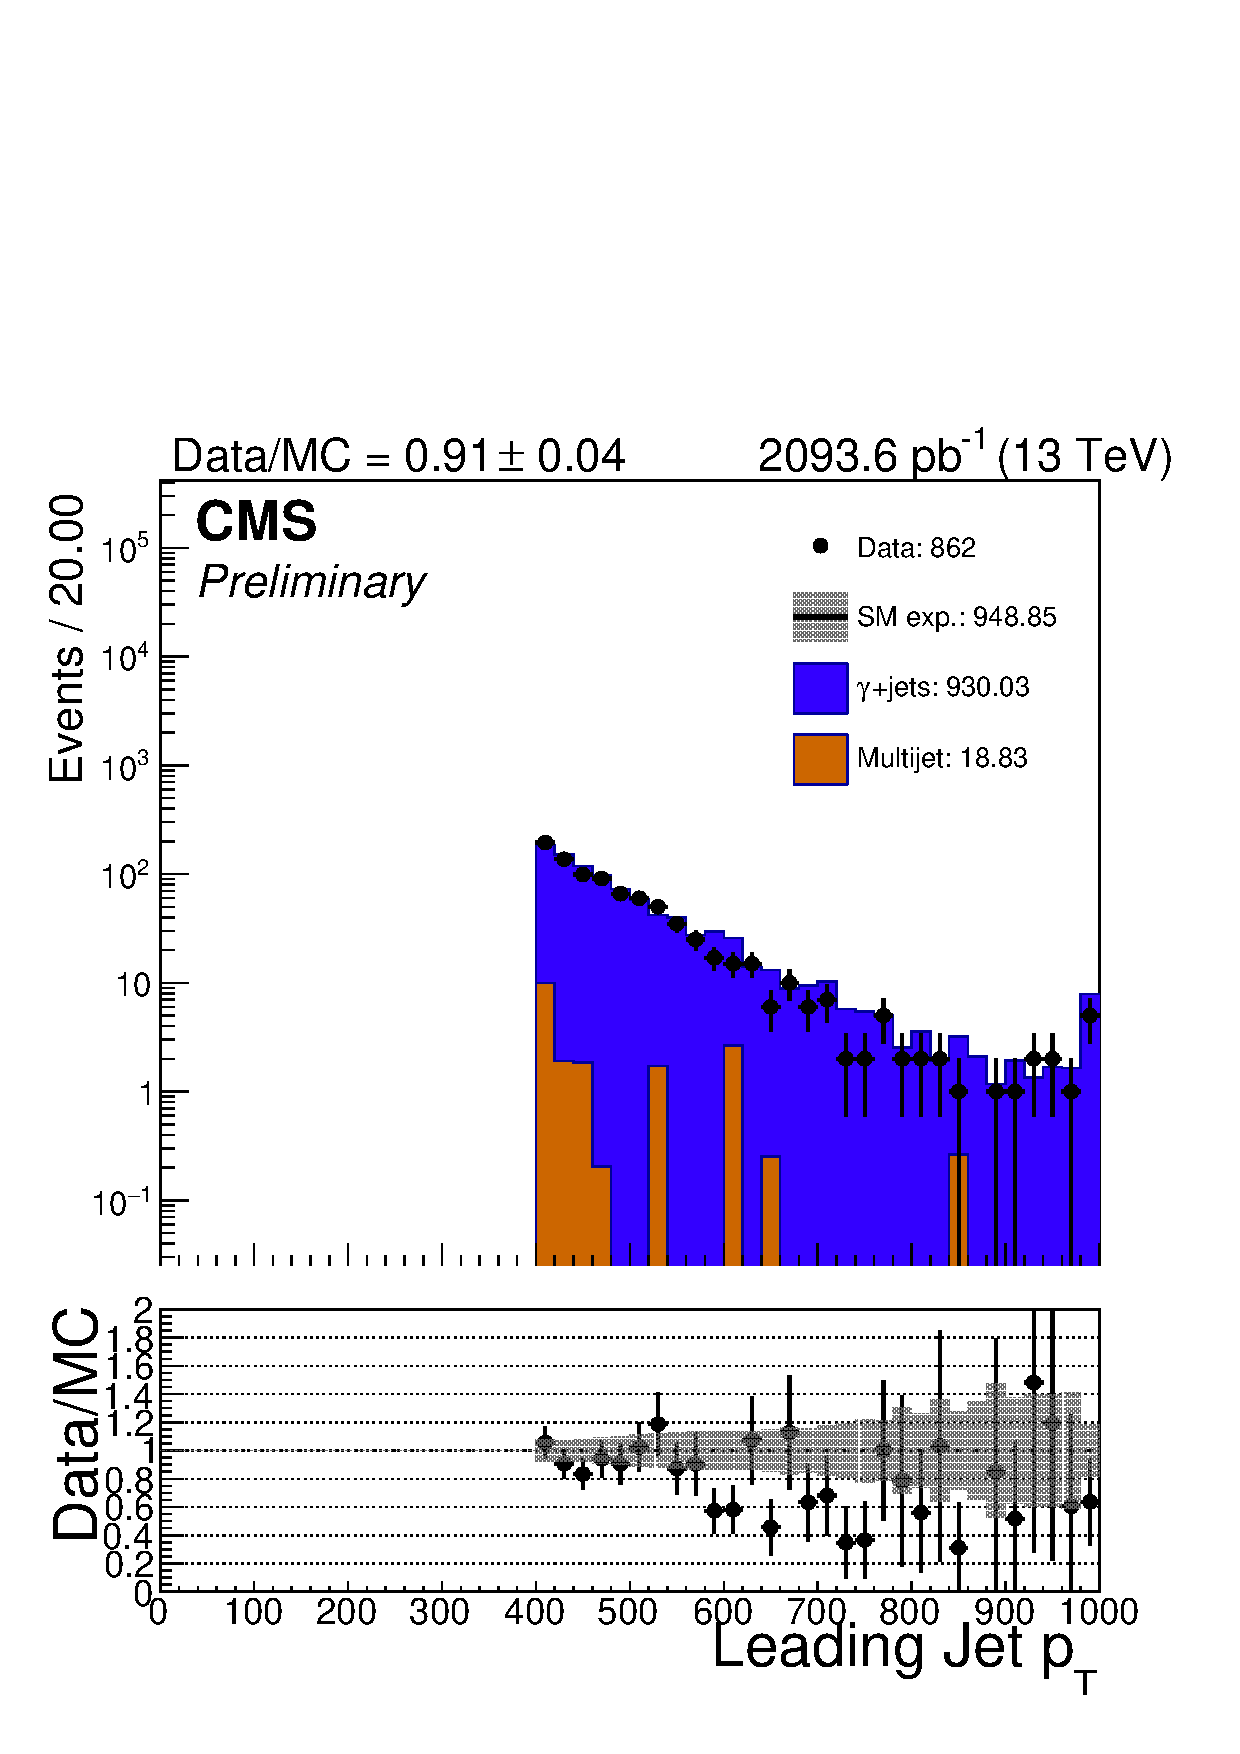
\includegraphics[width=0.5\textwidth]{figures/distributions/SinglePhoton/jet_pt[0]_eq1j.pdf}} ~~
        \subfigure {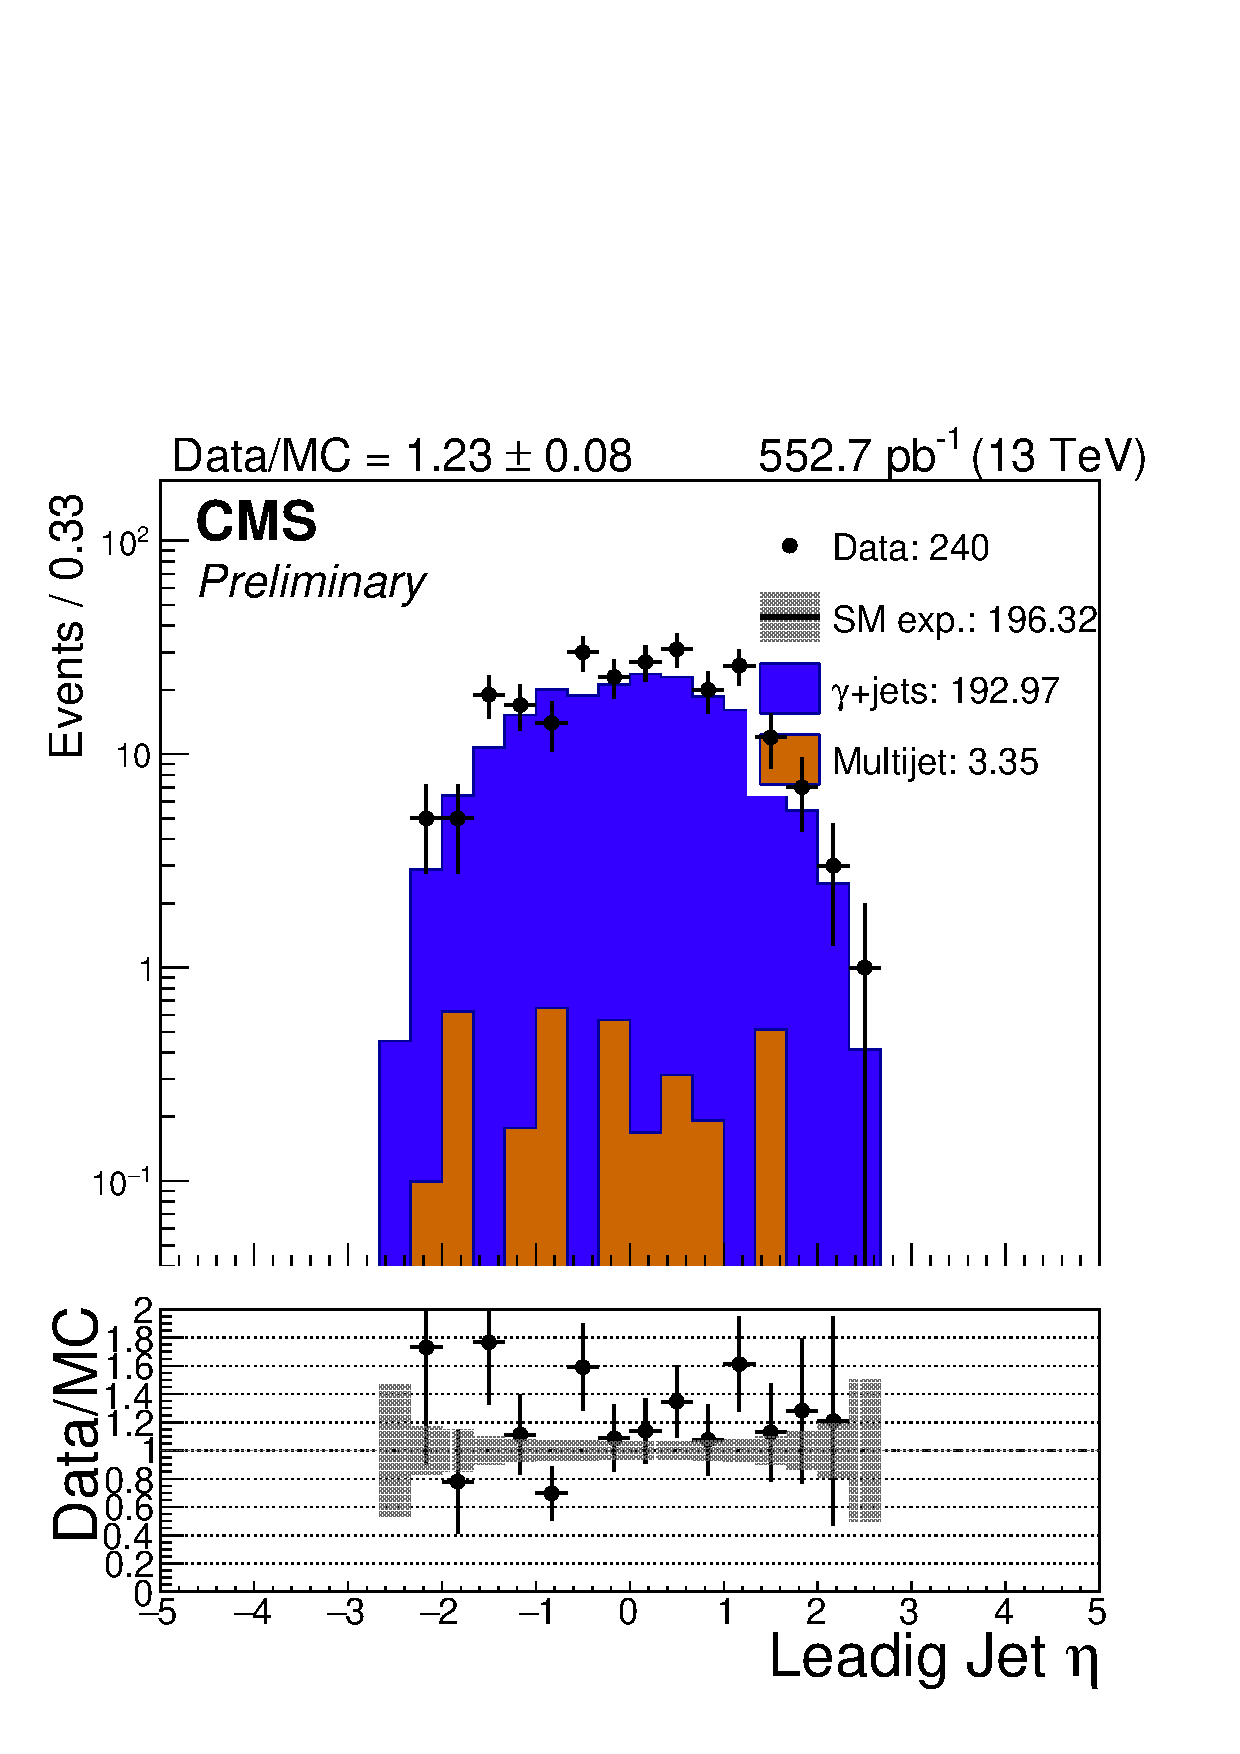
\includegraphics[width=0.5\textwidth]{figures/distributions/SinglePhoton/jet_eta[0]_eq1j.pdf}} \\
        \subfigure {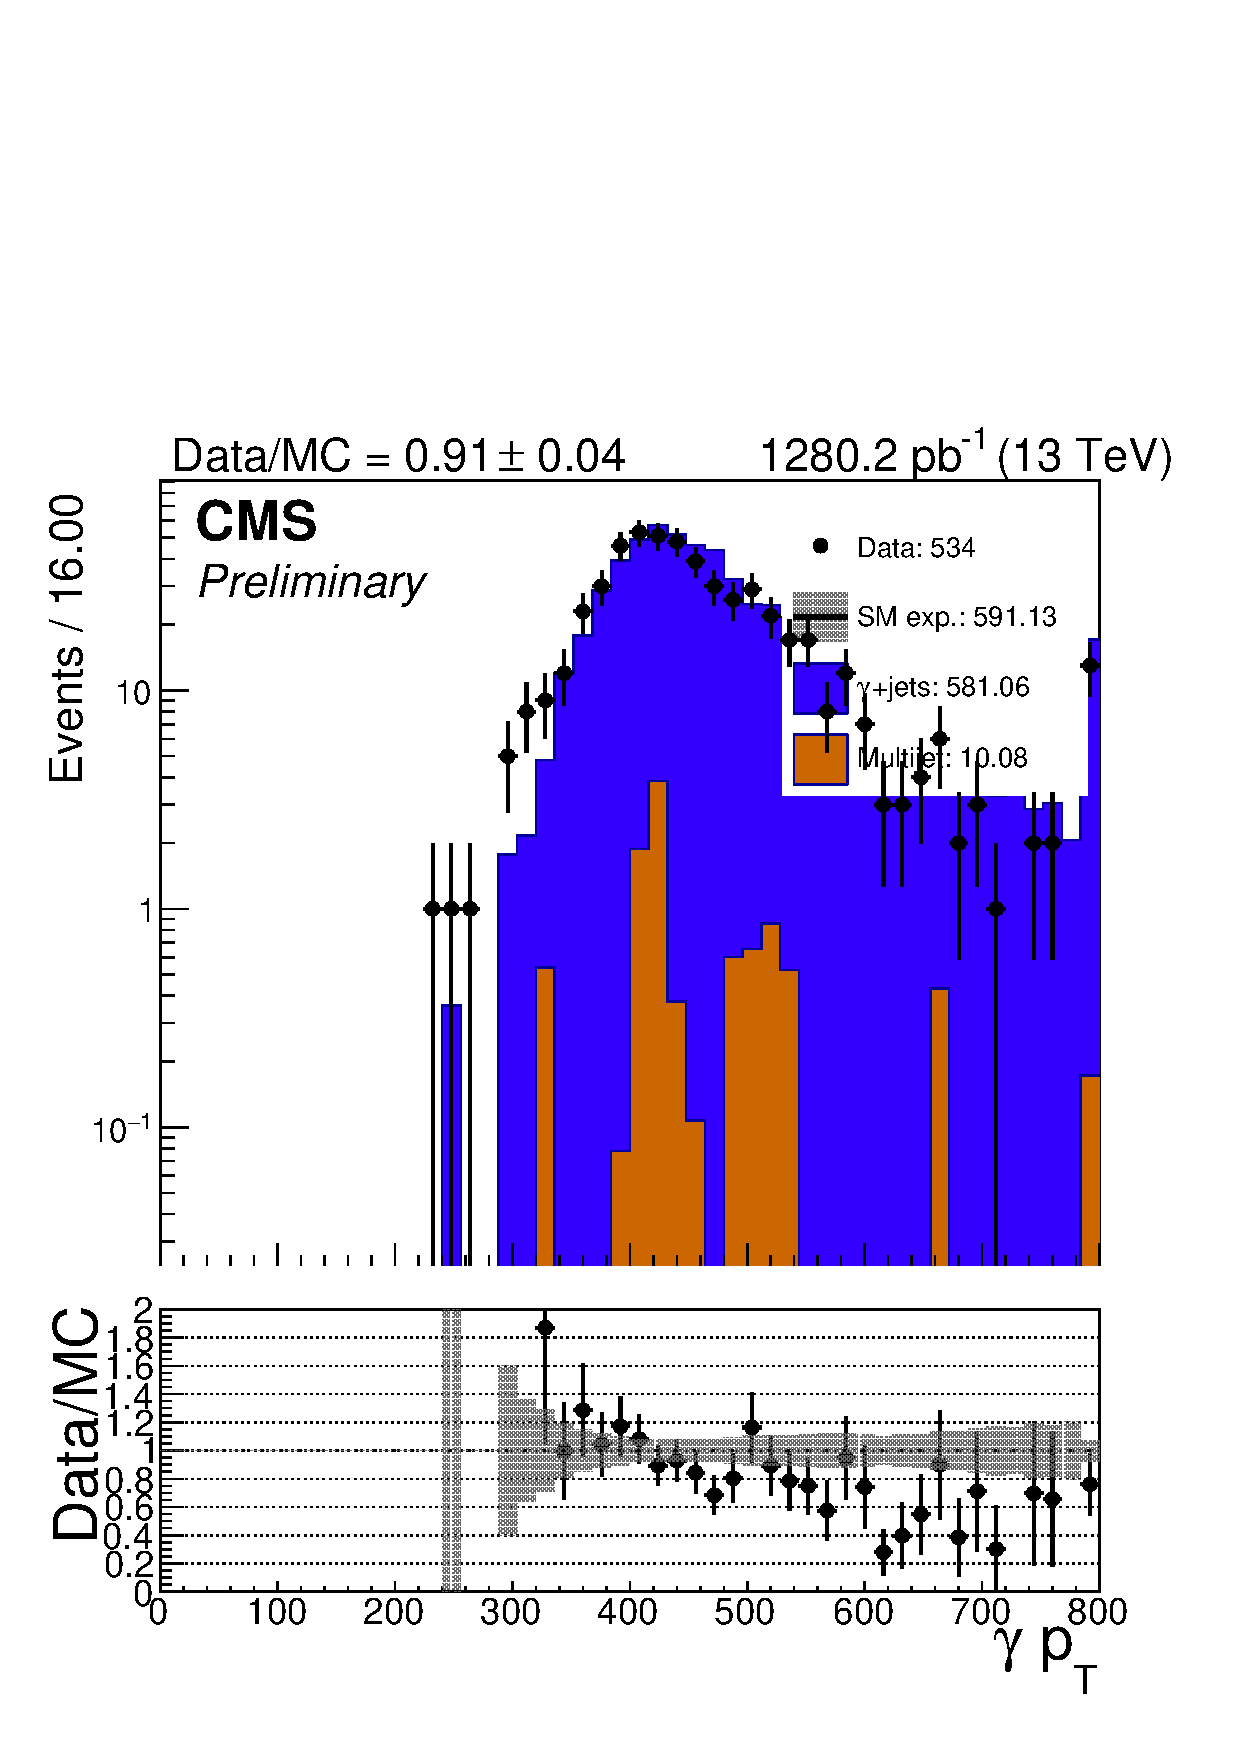
\includegraphics[width=0.5\textwidth]{figures/distributions/SinglePhoton/gamma_pt[0]_eq1j.pdf}} ~~
        \subfigure {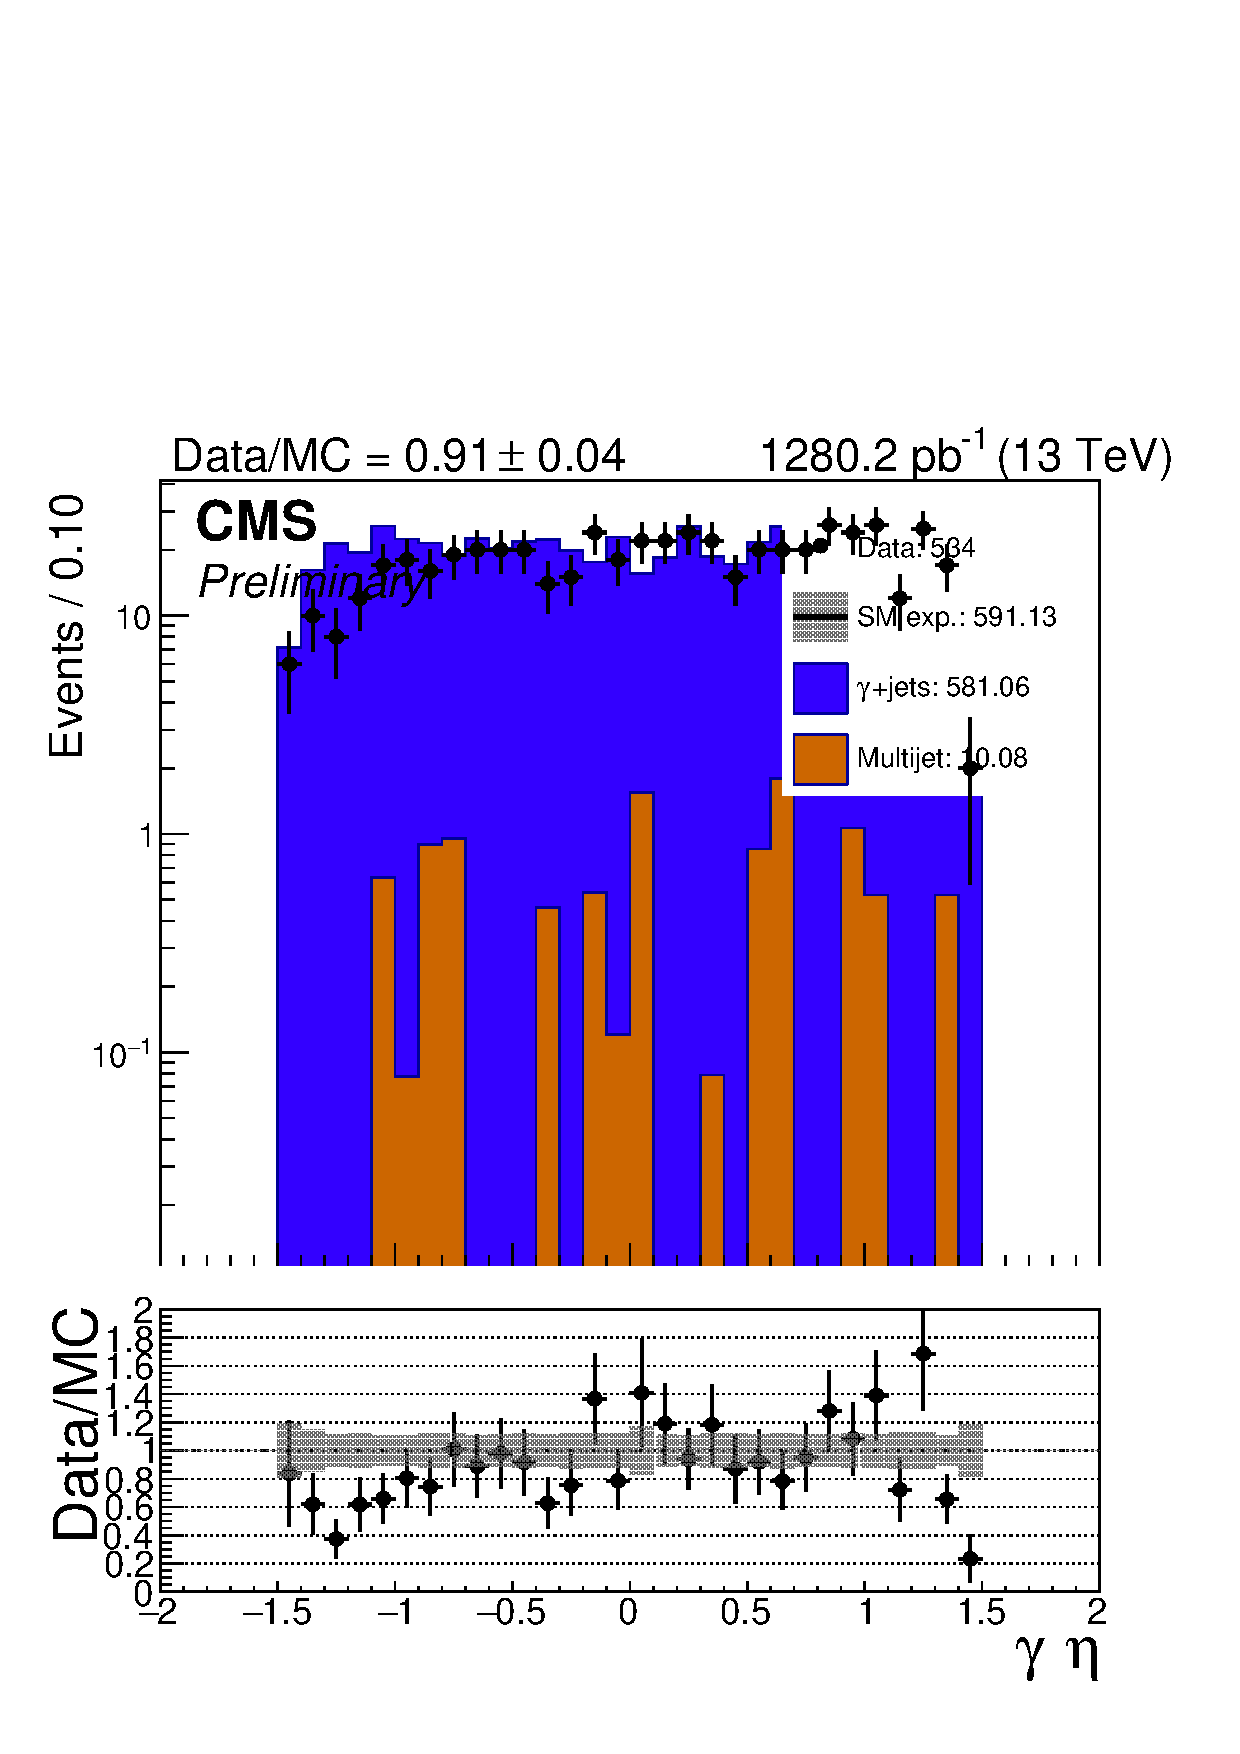
\includegraphics[width=0.5\textwidth]{figures/distributions/SinglePhoton/gamma_eta[0]_eq1j.pdf}} \\
        \caption{Key analysis variables for single photon control region (monojet bins)}
        \label{fig:distribution_singlephoton_mono}
    \end{center}
\end{figure}

\clearpage

%%____________________________________________________________________________||
\subsection{Breakdown of SM backgrounds in the hadronic signal
  region\label{sec:bkgd-comp}}

In the absence of multijet events from QCD, the remaining significant
backgrounds in the signal region are expected to stem from SM
processes with genuine \met in the final state. For the low jet
multiplicity categories, the largest backgrounds with genuine \met are
 from the associated production of W or Z bosons with jets,
followed by either the weak decays \znunu\ or \wtaunu, where the
$\tau$ decays hadronically and is identified as a jet, or by leptonic
decays that are outside acceptance or not rejected by the dedicated
electron or muon vetoes. For the higher jet multiplicity categories,
top quark production followed by semileptonic weak top quark decay
becomes dominant. The relative contribution from \ttbar is depending on 
the jet multiplicity with increase importance for large jet multiplicities.

% A breakdown
% of the relative contributions of the SM backgrounds, as given by
% simulation, in the different (\njet, \nb, \scalht) bins can be found
% in Table~\ref{tab:backgrounds}. 
Tables showing the yields for these electroweak backgrounds can be seen in Table~\ref{tab:yields_ewk_sig}.
An overview of the three dominant channels, \ttbar, \zInv~ and W~+~jets, are shown in Tables \ref{tab:yields_tt_sig}, 
\ref{tab:yields_zinv_sig} and \ref{tab:yields_wjetstolnuht_sig} respectively for 1.28\ifb 
(yields for 3\ifb are in Appendix~\ref{app:yields3fb}). The contribution from
other sources, such as the single top and diboson channels, was found to be
negligible so are not shown.

%\begin{landscape}

\newpage
\begin{table}
\tiny
\centering
\topcaption{Yields for the Electroweak process in the signal region for 3\ifb. The letter ``a'' in jet \eg ``2a''  indicates the asymmetric jet bins.\label{tab:yields_ewk_sig}}
\begin{tabular}
{c|c|cccccccc}
	\hline\hline
   &     & \multicolumn{8}{c}{\scalht (\gev)} \\ 
	\njet & \nb & 200-250 & 250-300 & 300-350 & 350-400 & 400-500 & 500-600 & 600-800 & 800-$\infty$ \\ 
\hline
	1 & 0 & 7291.15 $\pm$40.24 & 2438.42 $\pm$20.04 & 975.06 $\pm$12.03 & 413.56 $\pm$6.92 & 307.19 $\pm$5.04 & 90.67 $\pm$2.39 & 40.27 $\pm$1.20 & 9.39 $\pm$0.79 \\ 
	1 & 1 & 252.78 $\pm$6.62 & 90.28 $\pm$3.54 & 41.28 $\pm$2.57 & 16.98 $\pm$1.34 & 14.50 $\pm$1.20 & 3.70 $\pm$0.78 & 1.90 $\pm$0.69 & 0.30 $\pm$0.67 \\ 
	2 & 0 & 899.02 $\pm$13.69 & 969.97 $\pm$13.33 & 652.84 $\pm$10.54 & 398.14 $\pm$7.34 & 363.80 $\pm$5.69 & 126.53 $\pm$2.86 & 62.69 $\pm$1.39 & 85.19 $\pm$1.46 \\ 
	2 & 1 & 99.89 $\pm$4.74 & 91.44 $\pm$4.22 & 62.33 $\pm$3.25 & 35.76 $\pm$2.28 & 29.90 $\pm$1.76 & 11.43 $\pm$1.09 & 6.57 $\pm$0.78 & 8.29 $\pm$0.77 \\ 
	2 & 2 & 5.32 $\pm$1.09 & 5.69 $\pm$1.00 & 3.86 $\pm$0.89 & 2.70 $\pm$0.82 & 1.89 $\pm$0.76 & 0.95 $\pm$0.69 & 0.31 $\pm$0.67 & 0.19 $\pm$0.66 \\ 
	3 & 0 & 1.42 $\pm$0.76 & 175.90 $\pm$5.79 & 481.02 $\pm$9.40 & 487.61 $\pm$8.71 & 586.13 $\pm$7.79 & 217.59 $\pm$3.89 & 124.73 $\pm$1.98 & 120.66 $\pm$1.73 \\ 
	3 & 1 & 0.55 $\pm$0.70 & 44.71 $\pm$3.37 & 102.19 $\pm$4.78 & 103.72 $\pm$4.77 & 101.44 $\pm$4.00 & 30.89 $\pm$1.81 & 17.15 $\pm$1.02 & 16.99 $\pm$0.95 \\ 
	3 & 2 & 0.00 $\pm$0.66 & 8.23 $\pm$1.55 & 19.52 $\pm$2.15 & 23.31 $\pm$2.40 & 16.46 $\pm$1.91 & 3.97 $\pm$0.86 & 1.98 $\pm$0.73 & 1.33 $\pm$0.68 \\ 
	3 & $\ge3$ & 0.00 $\pm$0.66 & 0.00 $\pm$0.66 & 0.11 $\pm$0.67 & 0.51 $\pm$0.69 & 0.31 $\pm$0.68 & 0.31 $\pm$0.68 & 0.07 $\pm$0.66 & 0.01 $\pm$0.66 \\ 
	4 & 0 & - & 1.32 $\pm$0.75 & 76.70 $\pm$4.06 & 215.86 $\pm$6.18 & 406.89 $\pm$7.10 & 196.72 $\pm$3.97 & 127.62 $\pm$2.20 & 102.43 $\pm$1.61 \\ 
	4 & 1 & - & 0.21 $\pm$0.67 & 29.14 $\pm$2.69 & 78.21 $\pm$4.32 & 137.53 $\pm$5.69 & 49.03 $\pm$2.86 & 28.43 $\pm$1.80 & 19.79 $\pm$1.17 \\ 
	4 & 2 & - & 0.00 $\pm$0.66 & 12.84 $\pm$1.99 & 29.62 $\pm$2.81 & 50.91 $\pm$3.54 & 14.31 $\pm$1.77 & 7.21 $\pm$1.39 & 3.94 $\pm$0.84 \\ 
	4 & $\ge3$ & - & 0.00 $\pm$0.66 & 0.20 $\pm$0.68 & 1.62 $\pm$0.79 & 2.45 $\pm$0.86 & 1.35 $\pm$0.75 & 0.59 $\pm$0.70 & 0.10 $\pm$0.66 \\ 
	$\ge5$ & 0 & - & - & 0.00 $\pm$0.66 & 10.88 $\pm$1.52 & 115.00 $\pm$4.31 & 109.12 $\pm$3.61 & 101.33 $\pm$2.68 & 92.09 $\pm$2.03 \\ 
	$\ge5$ & 1 & - & - & 0.00 $\pm$0.66 & 7.36 $\pm$1.46 & 74.56 $\pm$4.31 & 62.14 $\pm$3.80 & 45.39 $\pm$2.96 & 35.90 $\pm$2.40 \\ 
	$\ge5$ & 2 & - & - & 0.00 $\pm$0.66 & 3.34 $\pm$1.13 & 30.88 $\pm$2.86 & 25.71 $\pm$2.59 & 20.95 $\pm$2.29 & 12.55 $\pm$1.70 \\ 
	$\ge5$ & $\ge3$ & - & - & 0.00 $\pm$0.66 & 0.93 $\pm$0.75 & 3.87 $\pm$1.20 & 3.31 $\pm$1.11 & 1.44 $\pm$0.77 & 1.51 $\pm$0.78 \\ 
	2a & 0 & 4622.92 $\pm$32.17 & 1354.85 $\pm$15.28 & 528.84 $\pm$9.30 & 219.56 $\pm$5.32 & 144.32 $\pm$3.56 & 37.08 $\pm$1.63 & 15.42 $\pm$0.90 & 14.10 $\pm$0.84 \\ 
	2a & 1 & 441.43 $\pm$9.80 & 121.34 $\pm$4.81 & 41.02 $\pm$2.58 & 17.98 $\pm$1.50 & 12.72 $\pm$1.22 & 2.76 $\pm$0.75 & 1.31 $\pm$0.68 & 1.05 $\pm$0.68 \\ 
	2a & 2 & 30.69 $\pm$2.48 & 6.02 $\pm$0.98 & 3.23 $\pm$0.86 & 1.47 $\pm$0.74 & 0.44 $\pm$0.68 & 0.07 $\pm$0.66 & 0.07 $\pm$0.66 & 0.03 $\pm$0.66 \\ 
	3a & 0 & 1259.29 $\pm$16.64 & 1259.13 $\pm$16.02 & 640.12 $\pm$10.98 & 212.64 $\pm$5.50 & 101.48 $\pm$3.21 & 20.08 $\pm$1.36 & 6.90 $\pm$0.77 & 6.12 $\pm$0.75 \\ 
	3a & 1 & 311.67 $\pm$8.88 & 307.52 $\pm$8.66 & 137.15 $\pm$5.60 & 43.47 $\pm$3.05 & 16.48 $\pm$1.68 & 1.92 $\pm$0.72 & 1.22 $\pm$0.71 & 0.73 $\pm$0.67 \\ 
	3a & 2 & 49.63 $\pm$3.52 & 56.27 $\pm$3.75 & 35.78 $\pm$3.07 & 7.23 $\pm$1.43 & 1.93 $\pm$0.76 & 0.40 $\pm$0.67 & 0.06 $\pm$0.66 & 0.03 $\pm$0.66 \\ 
	3a & $\ge3$ & 1.21 $\pm$0.77 & 0.98 $\pm$0.72 & 0.59 $\pm$0.71 & 0.01 $\pm$0.66 & 0.08 $\pm$0.67 & 0.00 $\pm$0.66 & 0.00 $\pm$0.66 & 0.00 $\pm$0.66 \\ 
	4a & 0 & - & 147.18 $\pm$5.58 & 368.00 $\pm$8.55 & 240.63 $\pm$6.56 & 134.45 $\pm$3.95 & 19.48 $\pm$1.40 & 3.72 $\pm$0.73 & 2.12 $\pm$0.69 \\ 
	4a & 1 & - & 56.40 $\pm$3.76 & 167.07 $\pm$6.80 & 96.71 $\pm$4.88 & 46.45 $\pm$3.21 & 3.39 $\pm$0.88 & 0.50 $\pm$0.67 & 0.40 $\pm$0.67 \\ 
	4a & 2 & - & 15.08 $\pm$2.01 & 53.45 $\pm$3.71 & 35.20 $\pm$3.12 & 15.09 $\pm$2.06 & 0.83 $\pm$0.70 & 0.02 $\pm$0.66 & 0.05 $\pm$0.66 \\ 
	4a & $\ge3$ & - & 0.32 $\pm$0.67 & 4.66 $\pm$1.29 & 2.24 $\pm$0.96 & 0.71 $\pm$0.72 & 0.19 $\pm$0.68 & 0.00 $\pm$0.66 & 0.01 $\pm$0.66 \\ 
	$\ge5$a & 0 & - & - & 35.71 $\pm$2.82 & 84.14 $\pm$4.12 & 112.10 $\pm$4.50 & 19.59 $\pm$1.60 & 5.37 $\pm$0.86 & 0.90 $\pm$0.68 \\ 
	$\ge5$a & 1 & - & - & 19.46 $\pm$2.14 & 64.43 $\pm$4.10 & 86.19 $\pm$4.76 & 13.17 $\pm$1.88 & 1.64 $\pm$0.77 & 0.15 $\pm$0.67 \\ 
	$\ge5$a & 2 & - & - & 12.99 $\pm$1.97 & 27.10 $\pm$2.74 & 45.10 $\pm$3.57 & 7.65 $\pm$1.51 & 0.85 $\pm$0.72 & 0.04 $\pm$0.66 \\ 
	$\ge5$a & $\ge3$ & - & - & 1.24 $\pm$0.79 & 4.16 $\pm$1.21 & 3.32 $\pm$1.09 & 2.11 $\pm$0.86 & 0.52 $\pm$0.70 & 0.00 $\pm$0.66 \\ 
	\hline
	\hline
\end{tabular}
\end{table}

\newpage
\begin{table}[h!]
\tiny
\centering
\topcaption{Yields for the \ttbar process in the signal region for 1.28\ifb. The letter ``a'' in jet \eg ``2a''  indicates the asymmetric jet bins.\label{tab:yields_tt_sig}}
\begin{tabular}
{c|c|cccccccc}
	\hline\hline
   &     & \multicolumn{8}{c}{\scalht (\gev)} \\ 
	\njet & \nb & 200-250 & 250-300 & 300-350 & 350-400 & 400-500 & 500-600 & 600-800 & 800-$\infty$ \\ 
\hline
	1 & 0 & 11.37 $\pm$1.14 & 2.89 $\pm$0.52 & 0.19 $\pm$0.27 & 0.01 $\pm$0.17 & 0.04 $\pm$0.14 & 0.00 $\pm$0.11 & 0.00 $\pm$0.11 & 0.00 $\pm$0.11 \\ 
	1 & 1 & 3.48 $\pm$0.53 & 1.17 $\pm$0.36 & 0.04 $\pm$0.12 & 0.25 $\pm$0.16 & 0.03 $\pm$0.12 & 0.00 $\pm$0.11 & 0.00 $\pm$0.11 & 0.00 $\pm$0.11 \\ 
	2 & 0 & 21.05 $\pm$1.52 & 16.86 $\pm$1.43 & 7.20 $\pm$0.90 & 3.13 $\pm$0.58 & 1.39 $\pm$0.43 & 0.03 $\pm$0.12 & 0.00 $\pm$0.12 & 0.14 $\pm$0.13 \\ 
	2 & 1 & 19.35 $\pm$1.48 & 14.60 $\pm$1.26 & 6.87 $\pm$0.85 & 2.76 $\pm$0.55 & 1.38 $\pm$0.38 & 0.63 $\pm$0.22 & 0.13 $\pm$0.14 & 0.05 $\pm$0.11 \\ 
	2 & 2 & 0.87 $\pm$0.32 & 0.57 $\pm$0.22 & 0.57 $\pm$0.20 & 0.46 $\pm$0.19 & 0.30 $\pm$0.17 & 0.01 $\pm$0.11 & 0.00 $\pm$0.11 & 0.00 $\pm$0.11 \\ 
	3 & 0 & 0.20 $\pm$0.14 & 8.78 $\pm$1.05 & 16.56 $\pm$1.38 & 12.72 $\pm$1.21 & 12.26 $\pm$1.18 & 2.00 $\pm$0.45 & 0.87 $\pm$0.34 & 0.82 $\pm$0.24 \\ 
	3 & 1 & 0.21 $\pm$0.14 & 13.37 $\pm$1.29 & 26.51 $\pm$1.72 & 23.85 $\pm$1.69 & 16.17 $\pm$1.34 & 2.92 $\pm$0.53 & 0.91 $\pm$0.26 & 0.66 $\pm$0.20 \\ 
	3 & 2 & 0.00 $\pm$0.11 & 2.74 $\pm$0.59 & 6.24 $\pm$0.83 & 7.48 $\pm$0.93 & 4.97 $\pm$0.74 & 0.68 $\pm$0.22 & 0.24 $\pm$0.16 & 0.02 $\pm$0.11 \\ 
	3 & $\ge3$ & 0.00 $\pm$0.11 & 0.00 $\pm$0.11 & 0.01 $\pm$0.11 & 0.14 $\pm$0.13 & 0.12 $\pm$0.13 & 0.12 $\pm$0.13 & 0.00 $\pm$0.11 & 0.00 $\pm$0.11 \\ 
	4 & 0 & - & 0.13 $\pm$0.13 & 5.95 $\pm$0.84 & 15.20 $\pm$1.33 & 19.61 $\pm$1.54 & 5.16 $\pm$0.74 & 1.69 $\pm$0.46 & 0.64 $\pm$0.22 \\ 
	4 & 1 & - & 0.05 $\pm$0.12 & 9.27 $\pm$1.03 & 23.93 $\pm$1.66 & 39.33 $\pm$2.28 & 8.79 $\pm$1.05 & 3.59 $\pm$0.66 & 1.11 $\pm$0.35 \\ 
	4 & 2 & - & 0.00 $\pm$0.11 & 4.84 $\pm$0.79 & 11.03 $\pm$1.13 & 18.56 $\pm$1.46 & 4.44 $\pm$0.67 & 2.01 $\pm$0.52 & 0.73 $\pm$0.23 \\ 
	4 & $\ge3$ & - & 0.00 $\pm$0.11 & 0.09 $\pm$0.13 & 0.57 $\pm$0.21 & 0.82 $\pm$0.25 & 0.49 $\pm$0.19 & 0.22 $\pm$0.15 & 0.00 $\pm$0.11 \\ 
	$\ge5$ & 0 & - & - & 0.00 $\pm$0.11 & 1.23 $\pm$0.37 & 12.66 $\pm$1.24 & 9.58 $\pm$1.05 & 4.97 $\pm$0.78 & 2.62 $\pm$0.62 \\ 
	$\ge5$ & 1 & - & - & 0.00 $\pm$0.11 & 2.79 $\pm$0.56 & 25.02 $\pm$1.74 & 19.45 $\pm$1.53 & 11.46 $\pm$1.18 & 7.38 $\pm$0.96 \\ 
	$\ge5$ & 2 & - & - & 0.00 $\pm$0.11 & 1.36 $\pm$0.41 & 12.06 $\pm$1.18 & 9.59 $\pm$1.06 & 7.46 $\pm$0.93 & 3.94 $\pm$0.67 \\ 
	$\ge5$ & $\ge3$ & - & - & 0.00 $\pm$0.11 & 0.40 $\pm$0.19 & 1.61 $\pm$0.44 & 1.29 $\pm$0.39 & 0.44 $\pm$0.20 & 0.47 $\pm$0.20 \\ 
	2a & 0 & 93.50 $\pm$3.32 & 20.07 $\pm$1.53 & 3.98 $\pm$0.70 & 1.47 $\pm$0.38 & 0.65 $\pm$0.22 & 0.09 $\pm$0.13 & 0.22 $\pm$0.14 & 0.00 $\pm$0.11 \\ 
	2a & 1 & 72.37 $\pm$2.91 & 15.71 $\pm$1.35 & 2.81 $\pm$0.53 & 1.37 $\pm$0.37 & 0.62 $\pm$0.23 & 0.03 $\pm$0.11 & 0.00 $\pm$0.11 & 0.04 $\pm$0.12 \\ 
	2a & 2 & 3.69 $\pm$0.65 & 0.34 $\pm$0.16 & 0.21 $\pm$0.15 & 0.05 $\pm$0.12 & 0.00 $\pm$0.11 & 0.00 $\pm$0.11 & 0.00 $\pm$0.11 & 0.00 $\pm$0.11 \\ 
	3a & 0 & 61.61 $\pm$2.66 & 55.75 $\pm$2.57 & 22.33 $\pm$1.66 & 5.52 $\pm$0.82 & 1.60 $\pm$0.42 & 0.22 $\pm$0.14 & 0.00 $\pm$0.11 & 0.00 $\pm$0.11 \\ 
	3a & 1 & 90.64 $\pm$3.26 & 86.15 $\pm$3.21 & 34.65 $\pm$2.02 & 9.07 $\pm$1.04 & 2.62 $\pm$0.55 & 0.14 $\pm$0.13 & 0.23 $\pm$0.15 & 0.00 $\pm$0.11 \\ 
	3a & 2 & 17.29 $\pm$1.42 & 18.46 $\pm$1.46 & 10.50 $\pm$1.12 & 2.43 $\pm$0.54 & 0.28 $\pm$0.16 & 0.00 $\pm$0.11 & 0.00 $\pm$0.11 & 0.00 $\pm$0.11 \\ 
	3a & $\ge3$ & 0.47 $\pm$0.20 & 0.28 $\pm$0.16 & 0.25 $\pm$0.15 & 0.00 $\pm$0.11 & 0.03 $\pm$0.12 & 0.00 $\pm$0.11 & 0.00 $\pm$0.11 & 0.00 $\pm$0.11 \\ 
	4a & 0 & - & 11.31 $\pm$1.16 & 26.58 $\pm$1.76 & 14.18 $\pm$1.27 & 4.61 $\pm$0.72 & 0.71 $\pm$0.25 & 0.03 $\pm$0.11 & 0.00 $\pm$0.11 \\ 
	4a & 1 & - & 17.74 $\pm$1.46 & 54.46 $\pm$2.57 & 29.63 $\pm$1.88 & 12.83 $\pm$1.26 & 0.47 $\pm$0.23 & 0.00 $\pm$0.11 & 0.03 $\pm$0.11 \\ 
	4a & 2 & - & 5.10 $\pm$0.79 & 20.66 $\pm$1.54 & 13.80 $\pm$1.29 & 5.52 $\pm$0.83 & 0.23 $\pm$0.14 & 0.00 $\pm$0.11 & 0.00 $\pm$0.11 \\ 
	4a & $\ge3$ & - & 0.09 $\pm$0.12 & 1.89 $\pm$0.49 & 0.90 $\pm$0.32 & 0.30 $\pm$0.16 & 0.08 $\pm$0.13 & 0.00 $\pm$0.11 & 0.00 $\pm$0.11 \\ 
	$\ge5$a & 0 & - & - & 4.56 $\pm$0.76 & 9.27 $\pm$1.05 & 11.69 $\pm$1.16 & 1.35 $\pm$0.41 & 0.25 $\pm$0.15 & 0.00 $\pm$0.11 \\ 
	$\ge5$a & 1 & - & - & 7.06 $\pm$0.85 & 24.07 $\pm$1.69 & 31.24 $\pm$1.95 & 4.33 $\pm$0.73 & 0.38 $\pm$0.20 & 0.03 $\pm$0.12 \\ 
	$\ge5$a & 2 & - & - & 5.14 $\pm$0.79 & 10.97 $\pm$1.13 & 18.12 $\pm$1.49 & 2.97 $\pm$0.58 & 0.34 $\pm$0.17 & 0.00 $\pm$0.11 \\ 
	$\ge5$a & $\ge3$ & - & - & 0.53 $\pm$0.21 & 1.72 $\pm$0.44 & 1.31 $\pm$0.39 & 0.83 $\pm$0.26 & 0.22 $\pm$0.15 & 0.00 $\pm$0.11 \\ 
	\hline
	\hline
\end{tabular}
\end{table}

\newpage
\begin{table}
\tiny
\centering
\topcaption{Yields for the W process in the signal region for 3\ifb. The letter ``a'' in jet \eg ``2a''  indicates the asymmetric jet bins.\label{tab:yields_wjetstolnuht_sig}}
\begin{tabular}
{c|c|cccccccc}
	\hline\hline
   &     & \multicolumn{8}{c}{\scalht (\gev)} \\ 
	\njet & \nb & 200-250 & 250-300 & 300-350 & 350-400 & 400-500 & 500-600 & 600-800 & 800-$\infty$ \\ 
\hline
	1 & 0 & 2723.78 $\pm$33.30 & 808.48 $\pm$16.54 & 284.89 $\pm$9.58 & 97.93 $\pm$5.09 & 71.21 $\pm$3.46 & 16.37 $\pm$1.44 & 6.15 $\pm$0.68 & 0.96 $\pm$0.58 \\ 
	1 & 1 & 63.58 $\pm$4.85 & 19.51 $\pm$2.53 & 10.86 $\pm$2.06 & 2.60 $\pm$0.83 & 3.28 $\pm$0.85 & 0.84 $\pm$0.61 & 0.26 $\pm$0.57 & 0.02 $\pm$0.57 \\ 
	2 & 0 & 365.20 $\pm$11.45 & 374.98 $\pm$11.13 & 246.58 $\pm$8.83 & 140.95 $\pm$5.97 & 121.18 $\pm$4.27 & 38.38 $\pm$2.00 & 17.53 $\pm$0.88 & 23.53 $\pm$0.86 \\ 
	2 & 1 & 19.95 $\pm$2.64 & 20.05 $\pm$2.51 & 14.64 $\pm$2.07 & 8.54 $\pm$1.45 & 8.09 $\pm$1.12 & 2.82 $\pm$0.77 & 1.45 $\pm$0.59 & 2.12 $\pm$0.60 \\ 
	2 & 2 & 0.23 $\pm$0.60 & 0.70 $\pm$0.64 & 0.32 $\pm$0.60 & 0.19 $\pm$0.57 & 0.07 $\pm$0.57 & 0.33 $\pm$0.58 & 0.04 $\pm$0.57 & 0.04 $\pm$0.57 \\ 
	3 & 0 & 0.44 $\pm$0.63 & 62.97 $\pm$4.54 & 187.56 $\pm$7.66 & 195.06 $\pm$7.14 & 218.50 $\pm$5.88 & 74.08 $\pm$2.76 & 36.06 $\pm$1.14 & 33.26 $\pm$0.95 \\ 
	3 & 1 & 0.00 $\pm$0.57 & 4.48 $\pm$1.23 & 14.00 $\pm$2.17 & 19.95 $\pm$2.28 & 23.01 $\pm$1.95 & 7.69 $\pm$1.00 & 4.56 $\pm$0.64 & 4.10 $\pm$0.63 \\ 
	3 & 2 & 0.00 $\pm$0.57 & 0.46 $\pm$0.61 & 1.47 $\pm$0.76 & 2.73 $\pm$0.87 & 0.87 $\pm$0.62 & 0.48 $\pm$0.59 & 0.30 $\pm$0.57 & 0.30 $\pm$0.57 \\ 
	3 & $\ge3$ & 0.00 $\pm$0.57 & 0.00 $\pm$0.57 & 0.00 $\pm$0.57 & 0.00 $\pm$0.57 & 0.00 $\pm$0.57 & 0.00 $\pm$0.57 & 0.00 $\pm$0.57 & 0.00 $\pm$0.57 \\ 
	4 & 0 & - & 0.70 $\pm$0.64 & 30.90 $\pm$3.16 & 80.85 $\pm$4.65 & 156.72 $\pm$5.10 & 67.40 $\pm$2.69 & 41.50 $\pm$1.28 & 30.69 $\pm$0.92 \\ 
	4 & 1 & - & 0.00 $\pm$0.57 & 2.69 $\pm$1.01 & 8.26 $\pm$1.59 & 15.43 $\pm$1.47 & 9.42 $\pm$1.12 & 6.08 $\pm$0.67 & 4.75 $\pm$0.63 \\ 
	4 & 2 & - & 0.00 $\pm$0.57 & 0.43 $\pm$0.61 & 2.06 $\pm$0.82 & 1.67 $\pm$0.72 & 0.88 $\pm$0.61 & 0.52 $\pm$0.58 & 0.48 $\pm$0.57 \\ 
	4 & $\ge3$ & - & 0.00 $\pm$0.57 & 0.00 $\pm$0.57 & 0.00 $\pm$0.57 & 0.16 $\pm$0.57 & 0.00 $\pm$0.57 & 0.03 $\pm$0.57 & 0.06 $\pm$0.57 \\ 
	$\ge5$ & 0 & - & - & 0.00 $\pm$0.57 & 3.95 $\pm$1.13 & 38.35 $\pm$2.72 & 34.42 $\pm$2.08 & 34.52 $\pm$1.47 & 29.17 $\pm$0.91 \\ 
	$\ge5$ & 1 & - & - & 0.00 $\pm$0.57 & 0.17 $\pm$0.57 & 6.98 $\pm$1.15 & 7.51 $\pm$1.07 & 6.67 $\pm$0.83 & 6.57 $\pm$0.66 \\ 
	$\ge5$ & 2 & - & - & 0.00 $\pm$0.57 & 0.00 $\pm$0.57 & 0.90 $\pm$0.64 & 1.10 $\pm$0.66 & 1.24 $\pm$0.61 & 0.86 $\pm$0.58 \\ 
	$\ge5$ & $\ge3$ & - & - & 0.00 $\pm$0.57 & 0.00 $\pm$0.57 & 0.00 $\pm$0.57 & 0.20 $\pm$0.57 & 0.04 $\pm$0.57 & 0.07 $\pm$0.57 \\ 
	2a & 0 & 1869.70 $\pm$26.61 & 487.25 $\pm$12.58 & 184.72 $\pm$7.69 & 67.56 $\pm$4.20 & 38.33 $\pm$2.56 & 9.64 $\pm$1.13 & 2.96 $\pm$0.61 & 2.22 $\pm$0.60 \\ 
	2a & 1 & 95.40 $\pm$5.77 & 27.31 $\pm$2.99 & 10.31 $\pm$1.83 & 2.48 $\pm$0.79 & 3.63 $\pm$0.88 & 0.39 $\pm$0.58 & 0.26 $\pm$0.57 & 0.11 $\pm$0.57 \\ 
	2a & 2 & 6.04 $\pm$1.53 & 1.01 $\pm$0.69 & 0.82 $\pm$0.66 & 0.83 $\pm$0.64 & 0.03 $\pm$0.57 & 0.00 $\pm$0.57 & 0.04 $\pm$0.57 & 0.00 $\pm$0.57 \\ 
	3a & 0 & 495.03 $\pm$13.38 & 489.10 $\pm$13.07 & 250.43 $\pm$8.96 & 71.06 $\pm$4.23 & 32.06 $\pm$2.37 & 5.54 $\pm$0.96 & 1.35 $\pm$0.59 & 1.10 $\pm$0.59 \\ 
	3a & 1 & 39.85 $\pm$3.90 & 41.54 $\pm$3.69 & 20.05 $\pm$2.49 & 8.01 $\pm$1.55 & 3.24 $\pm$0.84 & 0.61 $\pm$0.59 & 0.17 $\pm$0.57 & 0.06 $\pm$0.57 \\ 
	3a & 2 & 2.18 $\pm$0.86 & 4.22 $\pm$1.28 & 4.92 $\pm$1.43 & 0.37 $\pm$0.60 & 0.10 $\pm$0.57 & 0.17 $\pm$0.57 & 0.00 $\pm$0.57 & 0.00 $\pm$0.57 \\ 
	3a & $\ge3$ & 0.00 $\pm$0.57 & 0.00 $\pm$0.57 & 0.00 $\pm$0.57 & 0.00 $\pm$0.57 & 0.00 $\pm$0.57 & 0.00 $\pm$0.57 & 0.00 $\pm$0.57 & 0.00 $\pm$0.57 \\ 
	4a & 0 & - & 56.78 $\pm$4.34 & 135.92 $\pm$6.60 & 94.50 $\pm$5.13 & 47.09 $\pm$2.86 & 5.96 $\pm$1.00 & 0.78 $\pm$0.58 & 0.38 $\pm$0.57 \\ 
	4a & 1 & - & 4.61 $\pm$1.28 & 16.96 $\pm$2.89 & 11.23 $\pm$1.80 & 4.87 $\pm$0.96 & 0.84 $\pm$0.61 & 0.15 $\pm$0.57 & 0.07 $\pm$0.57 \\ 
	4a & 2 & - & 0.75 $\pm$0.65 & 1.05 $\pm$0.67 & 0.66 $\pm$0.62 & 0.33 $\pm$0.59 & 0.10 $\pm$0.57 & 0.01 $\pm$0.57 & 0.00 $\pm$0.57 \\ 
	4a & $\ge3$ & - & 0.00 $\pm$0.57 & 0.00 $\pm$0.57 & 0.00 $\pm$0.57 & 0.00 $\pm$0.57 & 0.00 $\pm$0.57 & 0.00 $\pm$0.57 & 0.00 $\pm$0.57 \\ 
	$\ge5$a & 0 & - & - & 11.73 $\pm$1.93 & 29.11 $\pm$2.92 & 43.04 $\pm$3.21 & 7.37 $\pm$1.08 & 1.72 $\pm$0.67 & 0.27 $\pm$0.57 \\ 
	$\ge5$a & 1 & - & - & 0.88 $\pm$0.66 & 2.32 $\pm$0.83 & 6.38 $\pm$1.21 & 1.24 $\pm$0.67 & 0.22 $\pm$0.57 & 0.01 $\pm$0.57 \\ 
	$\ge5$a & 2 & - & - & 0.58 $\pm$0.63 & 0.32 $\pm$0.59 & 0.67 $\pm$0.62 & 0.02 $\pm$0.57 & 0.00 $\pm$0.57 & 0.00 $\pm$0.57 \\ 
	$\ge5$a & $\ge3$ & - & - & 0.00 $\pm$0.57 & 0.13 $\pm$0.58 & 0.00 $\pm$0.57 & 0.02 $\pm$0.57 & 0.00 $\pm$0.57 & 0.00 $\pm$0.57 \\ 
	\hline
	\hline
\end{tabular}
\end{table}

\newpage
\begin{table}[h!]
\tiny
\centering
\topcaption{Yields for the \zInv~ process in the signal region for 1.28\ifb. The letter ``a'' in jet \eg ``2a''  indicates the asymmetric jet bins.\label{tab:yields_zinv_sig}}
\begin{tabular}
{c|c|cccccccc}
	\hline\hline
   &     & \multicolumn{8}{c}{\scalht (\gev)} \\ 
	\njet & \nb & 200-250 & 250-300 & 300-350 & 350-400 & 400-500 & 500-600 & 600-800 & 800-$\infty$ \\ 
\hline
	1 & 0 & 1937.37 $\pm$9.57 & 692.55 $\pm$4.80 & 294.28 $\pm$3.09 & 134.66 $\pm$1.99 & 100.64 $\pm$1.56 & 31.70 $\pm$0.81 & 14.55 $\pm$0.41 & 3.60 $\pm$0.20 \\ 
	1 & 1 & 77.25 $\pm$1.85 & 29.02 $\pm$0.99 & 12.94 $\pm$0.64 & 5.88 $\pm$0.42 & 4.76 $\pm$0.34 & 1.24 $\pm$0.17 & 0.70 $\pm$0.12 & 0.12 $\pm$0.10 \\ 
	2 & 0 & 206.72 $\pm$2.82 & 237.00 $\pm$2.79 & 166.14 $\pm$2.28 & 106.61 $\pm$1.73 & 102.13 $\pm$1.55 & 37.58 $\pm$0.87 & 19.27 $\pm$0.44 & 26.17 $\pm$0.48 \\ 
	2 & 1 & 14.75 $\pm$0.79 & 15.86 $\pm$0.71 & 13.48 $\pm$0.65 & 8.86 $\pm$0.50 & 7.92 $\pm$0.43 & 3.04 $\pm$0.25 & 2.05 $\pm$0.17 & 2.58 $\pm$0.18 \\ 
	2 & 2 & 1.30 $\pm$0.22 & 1.56 $\pm$0.24 & 0.94 $\pm$0.19 & 0.61 $\pm$0.16 & 0.48 $\pm$0.13 & 0.25 $\pm$0.12 & 0.12 $\pm$0.10 & 0.06 $\pm$0.10 \\ 
	3 & 0 & 0.22 $\pm$0.11 & 39.41 $\pm$1.12 & 108.64 $\pm$1.87 & 112.10 $\pm$1.76 & 144.59 $\pm$1.83 & 59.23 $\pm$1.08 & 36.96 $\pm$0.61 & 36.47 $\pm$0.57 \\ 
	3 & 1 & 0.03 $\pm$0.10 & 3.79 $\pm$0.36 & 11.11 $\pm$0.58 & 11.90 $\pm$0.57 & 17.29 $\pm$0.65 & 6.98 $\pm$0.36 & 4.46 $\pm$0.22 & 4.84 $\pm$0.23 \\ 
	3 & 2 & 0.00 $\pm$0.09 & 0.58 $\pm$0.16 & 1.47 $\pm$0.23 & 1.30 $\pm$0.20 & 1.69 $\pm$0.21 & 0.81 $\pm$0.15 & 0.47 $\pm$0.11 & 0.42 $\pm$0.11 \\ 
	3 & $\ge3$ & 0.00 $\pm$0.09 & 0.00 $\pm$0.09 & 0.04 $\pm$0.10 & 0.08 $\pm$0.10 & 0.01 $\pm$0.09 & 0.01 $\pm$0.09 & 0.03 $\pm$0.09 & 0.00 $\pm$0.09 \\ 
	4 & 0 & - & 0.14 $\pm$0.11 & 13.59 $\pm$0.68 & 42.41 $\pm$1.11 & 87.13 $\pm$1.45 & 50.01 $\pm$1.00 & 35.06 $\pm$0.61 & 29.97 $\pm$0.52 \\ 
	4 & 1 & - & 0.04 $\pm$0.10 & 2.01 $\pm$0.27 & 5.91 $\pm$0.41 & 12.76 $\pm$0.55 & 8.11 $\pm$0.41 & 5.94 $\pm$0.27 & 5.31 $\pm$0.23 \\ 
	4 & 2 & - & 0.00 $\pm$0.09 & 0.46 $\pm$0.16 & 0.73 $\pm$0.17 & 2.45 $\pm$0.26 & 1.29 $\pm$0.22 & 0.85 $\pm$0.13 & 0.75 $\pm$0.12 \\ 
	4 & $\ge3$ & - & 0.00 $\pm$0.09 & 0.00 $\pm$0.09 & 0.13 $\pm$0.10 & 0.16 $\pm$0.10 & 0.09 $\pm$0.10 & 0.02 $\pm$0.09 & 0.02 $\pm$0.09 \\ 
	$\ge5$ & 0 & - & - & 0.00 $\pm$0.09 & 1.72 $\pm$0.23 & 20.05 $\pm$0.71 & 22.29 $\pm$0.69 & 23.54 $\pm$0.55 & 24.23 $\pm$0.47 \\ 
	$\ge5$ & 1 & - & - & 0.00 $\pm$0.09 & 0.28 $\pm$0.11 & 3.81 $\pm$0.31 & 3.86 $\pm$0.30 & 5.07 $\pm$0.27 & 5.13 $\pm$0.23 \\ 
	$\ge5$ & 2 & - & - & 0.00 $\pm$0.09 & 0.06 $\pm$0.10 & 0.73 $\pm$0.16 & 0.91 $\pm$0.16 & 0.95 $\pm$0.15 & 1.05 $\pm$0.13 \\ 
	$\ge5$ & $\ge3$ & - & - & 0.00 $\pm$0.09 & 0.00 $\pm$0.09 & 0.04 $\pm$0.10 & 0.04 $\pm$0.09 & 0.16 $\pm$0.10 & 0.14 $\pm$0.10 \\ 
	2a & 0 & 1081.21 $\pm$6.97 & 350.11 $\pm$3.38 & 142.84 $\pm$2.12 & 63.38 $\pm$1.34 & 44.57 $\pm$1.03 & 11.62 $\pm$0.48 & 5.10 $\pm$0.24 & 5.08 $\pm$0.23 \\ 
	2a & 1 & 75.27 $\pm$1.73 & 24.41 $\pm$0.88 & 10.30 $\pm$0.57 & 5.24 $\pm$0.40 & 3.26 $\pm$0.28 & 0.98 $\pm$0.17 & 0.45 $\pm$0.11 & 0.36 $\pm$0.11 \\ 
	2a & 2 & 6.83 $\pm$0.52 & 1.80 $\pm$0.25 & 0.82 $\pm$0.18 & 0.23 $\pm$0.11 & 0.17 $\pm$0.11 & 0.03 $\pm$0.09 & 0.01 $\pm$0.09 & 0.01 $\pm$0.09 \\ 
	3a & 0 & 264.48 $\pm$3.29 & 272.80 $\pm$3.00 & 143.94 $\pm$2.14 & 54.88 $\pm$1.25 & 28.02 $\pm$0.82 & 5.98 $\pm$0.38 & 2.37 $\pm$0.18 & 2.14 $\pm$0.17 \\ 
	3a & 1 & 25.33 $\pm$0.98 & 27.33 $\pm$0.93 & 15.32 $\pm$0.69 & 6.06 $\pm$0.42 & 3.03 $\pm$0.28 & 0.42 $\pm$0.12 & 0.22 $\pm$0.10 & 0.29 $\pm$0.11 \\ 
	3a & 2 & 2.95 $\pm$0.32 & 3.74 $\pm$0.35 & 2.67 $\pm$0.31 & 0.50 $\pm$0.14 & 0.50 $\pm$0.14 & 0.10 $\pm$0.10 & 0.02 $\pm$0.09 & 0.01 $\pm$0.09 \\ 
	3a & $\ge3$ & 0.04 $\pm$0.10 & 0.14 $\pm$0.11 & 0.00 $\pm$0.09 & 0.00 $\pm$0.09 & 0.00 $\pm$0.09 & 0.00 $\pm$0.09 & 0.00 $\pm$0.09 & 0.00 $\pm$0.09 \\ 
	4a & 0 & - & 27.26 $\pm$0.95 & 72.45 $\pm$1.51 & 48.17 $\pm$1.19 & 32.67 $\pm$0.91 & 5.06 $\pm$0.33 & 1.22 $\pm$0.15 & 0.77 $\pm$0.12 \\ 
	4a & 1 & - & 4.35 $\pm$0.38 & 9.58 $\pm$0.55 & 6.84 $\pm$0.45 & 4.91 $\pm$0.35 & 0.62 $\pm$0.14 & 0.15 $\pm$0.10 & 0.11 $\pm$0.10 \\ 
	4a & 2 & - & 1.01 $\pm$0.21 & 1.70 $\pm$0.24 & 0.94 $\pm$0.18 & 0.78 $\pm$0.15 & 0.08 $\pm$0.10 & 0.00 $\pm$0.09 & 0.02 $\pm$0.09 \\ 
	4a & $\ge3$ & - & 0.05 $\pm$0.10 & 0.10 $\pm$0.10 & 0.05 $\pm$0.10 & 0.00 $\pm$0.09 & 0.00 $\pm$0.09 & 0.00 $\pm$0.09 & 0.00 $\pm$0.09 \\ 
	$\ge5$a & 0 & - & - & 5.67 $\pm$0.44 & 14.21 $\pm$0.66 & 17.77 $\pm$0.68 & 3.86 $\pm$0.29 & 1.31 $\pm$0.17 & 0.27 $\pm$0.11 \\ 
	$\ge5$a & 1 & - & - & 0.86 $\pm$0.18 & 2.43 $\pm$0.28 & 2.81 $\pm$0.27 & 0.76 $\pm$0.15 & 0.22 $\pm$0.10 & 0.03 $\pm$0.09 \\ 
	$\ge5$a & 2 & - & - & 0.16 $\pm$0.11 & 0.46 $\pm$0.14 & 0.83 $\pm$0.17 & 0.28 $\pm$0.12 & 0.03 $\pm$0.09 & 0.02 $\pm$0.09 \\ 
	$\ge5$a & $\ge3$ & - & - & 0.00 $\pm$0.09 & 0.00 $\pm$0.09 & 0.11 $\pm$0.10 & 0.06 $\pm$0.10 & 0.00 $\pm$0.09 & 0.00 $\pm$0.09 \\ 
	\hline
	\hline
\end{tabular}
\end{table}


%%____________________________________________________________________________||
\newpage
\subsection{Yields in the control samples}

The yields in the \mj, \mmj, \ej, \eej and \gj control samples can be found in
Tables~\ref{tab:yields_ewk_mu}, \ref{tab:yields_ewk_mumu},
and \ref{tab:yields_ewk_gj} respectively for 1.28 \ifb (yields for 3\ifb are in Appendix~\ref{app:yields3fb}). 
The number of events in each of these regions is important to determine how these analysis regions can be extended. We require to 
each control region to have sufficiently populated control regions to enable a robust data driven background prediction.


\begin{table}[h!]
\tiny
\centering
\topcaption{Yields  in the \mj control region for 3.0\ifb. The letter ``a'' in jet \eg ``2a''  indicates the asymmetric jet bins.\label{tab:yields_ewk_mu}}
\begin{tabular}
{c|c|cccccccc}
	\hline\hline
   &     & \multicolumn{8}{c}{\scalht (\gev)} \\ 
	\njet & \nb & 200-250 & 250-300 & 300-350 & 350-400 & 400-500 & 500-600 & 600-800 & 800-$\infty$ \\ 
\hline
	1 & 0 & 4346.16 $\pm$40.68 & 1592.60 $\pm$22.75 & 692.78 $\pm$14.96 & 331.48 $\pm$9.23 & 266.59 $\pm$6.55 & 86.63 $\pm$3.11 & 42.70 $\pm$1.31 & 9.47 $\pm$0.77 \\ 
	1 & 1 & 176.85 $\pm$7.95 & 59.85 $\pm$4.23 & 28.35 $\pm$2.91 & 14.05 $\pm$1.86 & 11.54 $\pm$1.41 & 3.23 $\pm$0.84 & 2.24 $\pm$0.71 & 0.43 $\pm$0.66 \\ 
	2 & 0 & 471.52 $\pm$12.57 & 689.05 $\pm$14.87 & 637.02 $\pm$14.00 & 572.29 $\pm$11.83 & 718.87 $\pm$10.28 & 346.85 $\pm$5.76 & 297.17 $\pm$3.08 & 152.20 $\pm$1.89 \\ 
	2 & 1 & 95.74 $\pm$5.20 & 103.58 $\pm$5.45 & 84.33 $\pm$4.91 & 67.27 $\pm$4.10 & 92.15 $\pm$4.28 & 43.38 $\pm$2.58 & 36.22 $\pm$2.01 & 18.80 $\pm$1.41 \\ 
	2 & 2 & 4.24 $\pm$1.12 & 8.31 $\pm$1.54 & 4.30 $\pm$1.13 & 6.44 $\pm$1.27 & 9.18 $\pm$1.66 & 4.03 $\pm$1.15 & 3.95 $\pm$1.06 & 1.12 $\pm$0.72 \\ 
	3 & 0 & 1.35 $\pm$0.77 & 211.79 $\pm$8.25 & 443.28 $\pm$11.52 & 507.10 $\pm$11.23 & 767.36 $\pm$11.31 & 449.96 $\pm$7.21 & 413.35 $\pm$4.43 & 244.60 $\pm$2.97 \\ 
	3 & 1 & 1.59 $\pm$0.81 & 111.05 $\pm$5.76 & 237.40 $\pm$8.29 & 230.05 $\pm$7.84 & 284.89 $\pm$8.26 & 146.74 $\pm$5.75 & 121.29 $\pm$4.77 & 59.26 $\pm$3.08 \\ 
	3 & 2 & 0.42 $\pm$0.69 & 25.55 $\pm$2.66 & 75.23 $\pm$4.63 & 82.77 $\pm$5.03 & 107.47 $\pm$5.43 & 45.02 $\pm$3.55 & 31.32 $\pm$2.82 & 11.28 $\pm$1.65 \\ 
	3 & $\ge3$ & 0.00 $\pm$0.66 & 2.93 $\pm$1.20 & 2.59 $\pm$1.03 & 1.27 $\pm$0.78 & 5.27 $\pm$1.42 & 2.20 $\pm$0.93 & 0.77 $\pm$0.70 & 0.63 $\pm$0.70 \\ 
	4 & 0 & - & 0.65 $\pm$0.71 & 60.89 $\pm$4.20 & 186.92 $\pm$7.02 & 467.26 $\pm$9.81 & 326.71 $\pm$6.90 & 351.12 $\pm$5.68 & 218.97 $\pm$3.33 \\ 
	4 & 1 & - & 0.83 $\pm$0.73 & 61.14 $\pm$4.16 & 170.46 $\pm$6.86 & 385.68 $\pm$10.19 & 232.47 $\pm$7.69 & 195.99 $\pm$6.87 & 94.58 $\pm$4.21 \\ 
	4 & 2 & - & 0.48 $\pm$0.69 & 25.35 $\pm$2.71 & 89.53 $\pm$5.06 & 198.32 $\pm$7.46 & 117.77 $\pm$5.70 & 84.26 $\pm$4.68 & 40.10 $\pm$3.20 \\ 
	4 & $\ge3$ & - & 0.00 $\pm$0.66 & 2.19 $\pm$0.86 & 6.35 $\pm$1.47 & 15.17 $\pm$2.10 & 11.30 $\pm$1.95 & 7.87 $\pm$1.61 & 3.83 $\pm$1.17 \\ 
	$\ge5$ & 0 & - & - & 0.54 $\pm$0.70 & 12.14 $\pm$1.86 & 130.45 $\pm$5.53 & 193.91 $\pm$6.33 & 276.01 $\pm$6.44 & 249.37 $\pm$5.19 \\ 
	$\ge5$ & 1 & - & - & 1.15 $\pm$0.77 & 16.62 $\pm$2.19 & 190.79 $\pm$7.46 & 263.29 $\pm$8.51 & 334.02 $\pm$9.32 & 249.03 $\pm$7.79 \\ 
	$\ge5$ & 2 & - & - & 0.43 $\pm$0.69 & 7.76 $\pm$1.53 & 112.22 $\pm$5.61 & 160.15 $\pm$6.59 & 221.24 $\pm$7.85 & 155.55 $\pm$6.53 \\ 
	$\ge5$ & $\ge3$ & - & - & 0.00 $\pm$0.66 & 1.41 $\pm$0.80 & 13.60 $\pm$2.03 & 20.49 $\pm$2.48 & 29.88 $\pm$2.92 & 24.79 $\pm$2.71 \\ 
	2a & 0 & 4607.64 $\pm$40.47 & 2399.37 $\pm$27.92 & 1123.04 $\pm$18.56 & 488.82 $\pm$10.94 & 341.74 $\pm$7.30 & 93.38 $\pm$3.06 & 47.18 $\pm$1.43 & 9.45 $\pm$0.77 \\ 
	2a & 1 & 806.41 $\pm$15.61 & 330.99 $\pm$9.77 & 156.22 $\pm$6.68 & 58.22 $\pm$3.87 & 43.53 $\pm$3.06 & 11.36 $\pm$1.51 & 5.11 $\pm$0.89 & 1.13 $\pm$0.69 \\ 
	2a & 2 & 78.48 $\pm$4.71 & 37.04 $\pm$3.18 & 13.35 $\pm$1.82 & 5.84 $\pm$1.24 & 2.42 $\pm$0.86 & 0.97 $\pm$0.76 & 1.00 $\pm$0.72 & 0.42 $\pm$0.69 \\ 
	3a & 0 & 1095.83 $\pm$19.39 & 1454.90 $\pm$21.44 & 797.53 $\pm$15.70 & 400.67 $\pm$10.02 & 287.16 $\pm$6.78 & 73.12 $\pm$3.12 & 31.99 $\pm$1.45 & 6.98 $\pm$0.77 \\ 
	3a & 1 & 605.88 $\pm$13.19 & 781.84 $\pm$15.02 & 376.38 $\pm$10.31 & 145.18 $\pm$6.15 & 88.67 $\pm$4.49 & 19.84 $\pm$1.98 & 8.42 $\pm$1.33 & 0.70 $\pm$0.67 \\ 
	3a & 2 & 162.51 $\pm$6.71 & 231.77 $\pm$8.08 & 115.94 $\pm$5.63 & 42.12 $\pm$3.35 & 24.86 $\pm$2.60 & 5.73 $\pm$1.27 & 1.71 $\pm$0.76 & 0.22 $\pm$0.67 \\ 
	3a & $\ge3$ & 6.24 $\pm$1.46 & 7.89 $\pm$1.58 & 3.97 $\pm$1.17 & 1.00 $\pm$0.76 & 1.14 $\pm$0.74 & 0.48 $\pm$0.69 & 0.00 $\pm$0.66 & 0.00 $\pm$0.66 \\ 
	4a & 0 & - & 224.44 $\pm$8.28 & 406.63 $\pm$11.27 & 259.42 $\pm$8.37 & 192.48 $\pm$6.24 & 52.65 $\pm$2.86 & 18.97 $\pm$1.34 & 2.90 $\pm$0.70 \\ 
	4a & 1 & - & 210.63 $\pm$7.62 & 358.86 $\pm$10.03 & 226.29 $\pm$7.95 & 142.79 $\pm$6.25 & 24.00 $\pm$2.40 & 8.29 $\pm$1.42 & 1.63 $\pm$0.75 \\ 
	4a & 2 & - & 93.55 $\pm$5.16 & 171.23 $\pm$6.96 & 110.06 $\pm$5.54 & 60.90 $\pm$4.10 & 16.33 $\pm$2.22 & 3.34 $\pm$1.17 & 0.19 $\pm$0.67 \\ 
	4a & $\ge3$ & - & 4.68 $\pm$1.19 & 12.39 $\pm$1.90 & 8.96 $\pm$1.71 & 2.92 $\pm$1.07 & 0.74 $\pm$0.71 & 0.41 $\pm$0.69 & 0.00 $\pm$0.66 \\ 
	$\ge5$a & 0 & - & - & 30.76 $\pm$2.99 & 88.61 $\pm$5.02 & 131.59 $\pm$5.72 & 39.65 $\pm$2.78 & 17.35 $\pm$1.83 & 1.22 $\pm$0.67 \\ 
	$\ge5$a & 1 & - & - & 46.91 $\pm$3.69 & 128.31 $\pm$6.11 & 179.72 $\pm$7.03 & 51.34 $\pm$3.73 & 21.09 $\pm$2.41 & 1.75 $\pm$0.80 \\ 
	$\ge5$a & 2 & - & - & 20.97 $\pm$2.39 & 60.20 $\pm$4.15 & 111.31 $\pm$5.67 & 36.34 $\pm$3.23 & 9.64 $\pm$1.69 & 1.28 $\pm$0.78 \\ 
	$\ge5$a & $\ge3$ & - & - & 2.35 $\pm$1.08 & 7.69 $\pm$1.59 & 7.74 $\pm$1.57 & 4.73 $\pm$1.36 & 1.92 $\pm$0.85 & 0.01 $\pm$0.66 \\ 
	\hline
	\hline
\end{tabular}
\end{table}

\newpage
\begin{table}[h!]
\tiny
\centering
\topcaption{Yields  in the \mmj control region for 1.28\ifb. The letter ``a'' in jet \eg ``2a''  indicates the asymmetric jet bins.\label{tab:yields_ewk_mumu}}
\begin{tabular}
{c|c|cccccccc}
	\hline\hline
   &     & \multicolumn{8}{c}{\scalht (\gev)} \\ 
	\njet & \nb & 200-250 & 250-300 & 300-350 & 350-400 & 400-500 & 500-600 & 600-800 & 800-$\infty$ \\ 
\hline
	1 & 0 & 255.86 $\pm$4.95 & 102.05 $\pm$3.01 & 45.27 $\pm$1.94 & 22.98 $\pm$1.22 & 17.90 $\pm$0.70 & 5.70 $\pm$0.28 & 2.84 $\pm$0.20 & 0.61 $\pm$0.17 \\ 
	1 & 1 & 13.53 $\pm$1.12 & 5.25 $\pm$0.67 & 3.01 $\pm$0.54 & 1.11 $\pm$0.25 & 0.73 $\pm$0.19 & 0.21 $\pm$0.17 & 0.14 $\pm$0.17 & 0.05 $\pm$0.16 \\ 
	2 & 0 & 20.83 $\pm$1.38 & 30.86 $\pm$1.64 & 32.26 $\pm$1.64 & 26.94 $\pm$1.24 & 34.55 $\pm$0.79 & 18.50 $\pm$0.45 & 15.34 $\pm$0.32 & 8.88 $\pm$0.30 \\ 
	2 & 1 & 2.58 $\pm$0.50 & 3.52 $\pm$0.57 & 3.72 $\pm$0.57 & 3.07 $\pm$0.46 & 3.79 $\pm$0.31 & 1.92 $\pm$0.26 & 1.57 $\pm$0.21 & 0.82 $\pm$0.17 \\ 
	2 & 2 & 0.08 $\pm$0.17 & 0.38 $\pm$0.20 & 0.23 $\pm$0.19 & 0.49 $\pm$0.21 & 0.13 $\pm$0.17 & 0.07 $\pm$0.16 & 0.09 $\pm$0.16 & 0.02 $\pm$0.16 \\ 
	3 & 0 & 0.05 $\pm$0.17 & 6.74 $\pm$0.78 & 15.83 $\pm$1.14 & 20.68 $\pm$1.10 & 31.37 $\pm$0.79 & 20.17 $\pm$0.47 & 19.65 $\pm$0.36 & 12.91 $\pm$0.30 \\ 
	3 & 1 & 0.00 $\pm$0.16 & 0.77 $\pm$0.25 & 2.81 $\pm$0.53 & 2.59 $\pm$0.39 & 6.14 $\pm$0.58 & 3.07 $\pm$0.27 & 2.98 $\pm$0.25 & 1.88 $\pm$0.19 \\ 
	3 & 2 & 0.00 $\pm$0.16 & 0.28 $\pm$0.19 & 0.56 $\pm$0.22 & 1.08 $\pm$0.28 & 1.29 $\pm$0.35 & 0.72 $\pm$0.23 & 0.29 $\pm$0.17 & 0.30 $\pm$0.19 \\ 
	3 & $\ge3$ & 0.00 $\pm$0.16 & 0.01 $\pm$0.16 & 0.00 $\pm$0.16 & 0.08 $\pm$0.17 & 0.02 $\pm$0.16 & 0.00 $\pm$0.16 & 0.00 $\pm$0.16 & 0.01 $\pm$0.16 \\ 
	4 & 0 & - & 0.00 $\pm$0.16 & 2.98 $\pm$0.54 & 5.90 $\pm$0.67 & 15.94 $\pm$0.68 & 12.79 $\pm$0.42 & 13.63 $\pm$0.33 & 10.50 $\pm$0.29 \\ 
	4 & 1 & - & 0.00 $\pm$0.16 & 0.31 $\pm$0.19 & 1.11 $\pm$0.27 & 3.35 $\pm$0.44 & 3.05 $\pm$0.39 & 3.06 $\pm$0.27 & 2.00 $\pm$0.19 \\ 
	4 & 2 & - & 0.00 $\pm$0.16 & 0.00 $\pm$0.16 & 0.63 $\pm$0.24 & 1.37 $\pm$0.36 & 0.77 $\pm$0.23 & 0.66 $\pm$0.20 & 0.41 $\pm$0.19 \\ 
	4 & $\ge3$ & - & 0.00 $\pm$0.16 & 0.00 $\pm$0.16 & 0.00 $\pm$0.16 & 0.03 $\pm$0.17 & 0.02 $\pm$0.16 & 0.03 $\pm$0.16 & 0.03 $\pm$0.16 \\ 
	$\ge5$ & 0 & - & - & 0.00 $\pm$0.16 & 0.09 $\pm$0.17 & 2.91 $\pm$0.37 & 4.39 $\pm$0.29 & 7.96 $\pm$0.33 & 8.96 $\pm$0.28 \\ 
	$\ge5$ & 1 & - & - & 0.00 $\pm$0.16 & 0.03 $\pm$0.17 & 1.37 $\pm$0.29 & 1.85 $\pm$0.37 & 2.15 $\pm$0.27 & 2.87 $\pm$0.36 \\ 
	$\ge5$ & 2 & - & - & 0.00 $\pm$0.16 & 0.03 $\pm$0.17 & 0.51 $\pm$0.22 & 0.42 $\pm$0.19 & 0.89 $\pm$0.26 & 1.06 $\pm$0.26 \\ 
	$\ge5$ & $\ge3$ & - & - & 0.00 $\pm$0.16 & 0.00 $\pm$0.16 & 0.00 $\pm$0.16 & 0.07 $\pm$0.17 & 0.28 $\pm$0.20 & 0.05 $\pm$0.16 \\ 
	2a & 0 & 207.84 $\pm$4.48 & 116.59 $\pm$3.29 & 60.10 $\pm$2.27 & 28.77 $\pm$1.39 & 18.49 $\pm$0.60 & 6.07 $\pm$0.29 & 2.97 $\pm$0.21 & 0.64 $\pm$0.17 \\ 
	2a & 1 & 23.33 $\pm$1.50 & 11.52 $\pm$1.04 & 6.84 $\pm$0.81 & 2.38 $\pm$0.38 & 1.58 $\pm$0.22 & 0.85 $\pm$0.24 & 0.26 $\pm$0.17 & 0.06 $\pm$0.16 \\ 
	2a & 2 & 3.24 $\pm$0.60 & 1.60 $\pm$0.39 & 0.24 $\pm$0.19 & 0.02 $\pm$0.16 & 0.06 $\pm$0.16 & 0.02 $\pm$0.16 & 0.01 $\pm$0.16 & 0.00 $\pm$0.16 \\ 
	3a & 0 & 38.65 $\pm$1.91 & 55.65 $\pm$2.29 & 29.70 $\pm$1.61 & 17.04 $\pm$1.03 & 14.80 $\pm$0.60 & 3.91 $\pm$0.25 & 2.07 $\pm$0.21 & 0.34 $\pm$0.17 \\ 
	3a & 1 & 7.29 $\pm$0.87 & 7.64 $\pm$0.89 & 5.45 $\pm$0.71 & 2.81 $\pm$0.46 & 2.05 $\pm$0.27 & 0.61 $\pm$0.19 & 0.41 $\pm$0.19 & 0.04 $\pm$0.17 \\ 
	3a & 2 & 1.81 $\pm$0.43 & 3.51 $\pm$0.67 & 1.83 $\pm$0.48 & 0.49 $\pm$0.20 & 0.63 $\pm$0.23 & 0.06 $\pm$0.16 & 0.01 $\pm$0.16 & 0.00 $\pm$0.16 \\ 
	3a & $\ge3$ & 0.05 $\pm$0.17 & 0.32 $\pm$0.20 & 0.06 $\pm$0.17 & 0.01 $\pm$0.16 & 0.01 $\pm$0.16 & 0.00 $\pm$0.16 & 0.00 $\pm$0.16 & 0.00 $\pm$0.16 \\ 
	4a & 0 & - & 5.71 $\pm$0.70 & 10.53 $\pm$0.92 & 8.46 $\pm$0.72 & 6.80 $\pm$0.44 & 2.22 $\pm$0.23 & 1.03 $\pm$0.20 & 0.16 $\pm$0.17 \\ 
	4a & 1 & - & 1.55 $\pm$0.40 & 3.34 $\pm$0.60 & 1.80 $\pm$0.36 & 2.14 $\pm$0.39 & 0.47 $\pm$0.19 & 0.26 $\pm$0.18 & 0.01 $\pm$0.16 \\ 
	4a & 2 & - & 0.24 $\pm$0.19 & 0.79 $\pm$0.26 & 0.48 $\pm$0.21 & 1.12 $\pm$0.37 & 0.33 $\pm$0.20 & 0.13 $\pm$0.18 & 0.19 $\pm$0.19 \\ 
	4a & $\ge3$ & - & 0.00 $\pm$0.16 & 0.01 $\pm$0.16 & 0.00 $\pm$0.16 & 0.00 $\pm$0.16 & 0.00 $\pm$0.16 & 0.00 $\pm$0.16 & 0.00 $\pm$0.16 \\ 
	$\ge5$a & 0 & - & - & 0.85 $\pm$0.26 & 1.88 $\pm$0.42 & 2.25 $\pm$0.27 & 1.04 $\pm$0.19 & 0.44 $\pm$0.17 & 0.10 $\pm$0.16 \\ 
	$\ge5$a & 1 & - & - & 0.19 $\pm$0.18 & 0.52 $\pm$0.22 & 1.57 $\pm$0.36 & 0.64 $\pm$0.24 & 0.19 $\pm$0.17 & 0.16 $\pm$0.18 \\ 
	$\ge5$a & 2 & - & - & 0.00 $\pm$0.16 & 0.26 $\pm$0.19 & 0.29 $\pm$0.19 & 0.15 $\pm$0.17 & 0.23 $\pm$0.19 & 0.00 $\pm$0.16 \\ 
	$\ge5$a & $\ge3$ & - & - & 0.00 $\pm$0.16 & 0.00 $\pm$0.16 & 0.24 $\pm$0.19 & 0.00 $\pm$0.16 & 0.00 $\pm$0.16 & 0.00 $\pm$0.16 \\ 
	\hline
	\hline
\end{tabular}
\end{table}

\newpage
\begin{table}[h!]
\tiny
\centering
\topcaption{Yields  in the \gj control region for 3.0\ifb. The letter ``a'' in jet \eg ``2a''  indicates the asymmetric jet bins.\label{tab:yields_ewk_gj}}
\begin{tabular}
{c|c|cccc}
	\hline\hline
   &     & \multicolumn{4}{c}{\scalht (\gev)} \\ 
	\njet & \nb & 400-500 & 500-600 & 600-800 & 800-$\infty$ \\ 
\hline
	1 & 0 & 550.71 $\pm$16.32 & 178.61 $\pm$8.10 & 93.67 $\pm$4.12 & 23.91 $\pm$2.01 \\ 
	1 & 1 & 22.97 $\pm$3.15 & 7.33 $\pm$1.66 & 4.52 $\pm$1.08 & 1.27 $\pm$0.85 \\ 
	2 & 0 & 260.59 $\pm$10.97 & 109.70 $\pm$6.32 & 71.72 $\pm$3.61 & 166.92 $\pm$5.04 \\ 
	2 & 1 & 21.74 $\pm$3.15 & 9.19 $\pm$1.96 & 4.92 $\pm$1.10 & 16.55 $\pm$1.74 \\ 
	2 & 2 & 1.63 $\pm$0.94 & 0.50 $\pm$0.77 & 0.24 $\pm$0.74 & 0.46 $\pm$0.75 \\ 
	3 & 0 & 407.84 $\pm$14.07 & 180.73 $\pm$8.12 & 112.58 $\pm$4.34 & 241.25 $\pm$5.98 \\ 
	3 & 1 & 40.80 $\pm$4.24 & 19.85 $\pm$2.71 & 9.77 $\pm$1.36 & 31.79 $\pm$2.29 \\ 
	3 & 2 & 3.64 $\pm$1.36 & 1.86 $\pm$0.89 & 1.24 $\pm$0.84 & 2.95 $\pm$0.99 \\ 
	3 & $\ge3$ & 0.00 $\pm$0.73 & 0.00 $\pm$0.73 & 0.04 $\pm$0.73 & 0.19 $\pm$0.74 \\ 
	4 & 0 & 219.39 $\pm$10.06 & 143.80 $\pm$7.37 & 124.20 $\pm$4.95 & 193.89 $\pm$5.41 \\ 
	4 & 1 & 32.41 $\pm$3.88 & 21.32 $\pm$2.92 & 16.71 $\pm$1.76 & 31.18 $\pm$2.24 \\ 
	4 & 2 & 7.82 $\pm$1.93 & 3.41 $\pm$1.10 & 3.58 $\pm$1.01 & 4.71 $\pm$1.08 \\ 
	4 & $\ge3$ & 0.05 $\pm$0.73 & 0.28 $\pm$0.76 & 0.12 $\pm$0.73 & 0.00 $\pm$0.73 \\ 
	$\ge5$ & 0 & 47.09 $\pm$5.57 & 63.76 $\pm$5.12 & 84.96 $\pm$4.29 & 148.69 $\pm$4.75 \\ 
	$\ge5$ & 1 & 8.28 $\pm$1.85 & 15.79 $\pm$2.54 & 21.15 $\pm$2.32 & 37.90 $\pm$2.46 \\ 
	$\ge5$ & 2 & 1.46 $\pm$0.91 & 2.67 $\pm$1.03 & 4.29 $\pm$1.14 & 6.95 $\pm$1.23 \\ 
	$\ge5$ & $\ge3$ & 0.00 $\pm$0.73 & 0.00 $\pm$0.73 & 0.12 $\pm$0.73 & 0.50 $\pm$0.75 \\ 
	2a & 0 & 128.17 $\pm$7.78 & 38.44 $\pm$3.83 & 21.99 $\pm$2.21 & 21.05 $\pm$1.85 \\ 
	2a & 1 & 7.35 $\pm$1.77 & 2.80 $\pm$1.01 & 0.66 $\pm$0.76 & 1.92 $\pm$0.90 \\ 
	2a & 2 & 0.00 $\pm$0.73 & 0.00 $\pm$0.73 & 0.00 $\pm$0.73 & 0.12 $\pm$0.73 \\ 
	3a & 0 & 81.16 $\pm$6.37 & 18.57 $\pm$2.62 & 6.75 $\pm$1.22 & 11.16 $\pm$1.46 \\ 
	3a & 1 & 11.01 $\pm$2.37 & 2.36 $\pm$0.96 & 1.31 $\pm$0.85 & 0.85 $\pm$0.78 \\ 
	3a & 2 & 1.54 $\pm$0.93 & 0.35 $\pm$0.77 & 0.09 $\pm$0.73 & 0.00 $\pm$0.73 \\ 
	3a & $\ge3$ & 0.00 $\pm$0.73 & 0.00 $\pm$0.73 & 0.00 $\pm$0.73 & 0.00 $\pm$0.73 \\ 
	4a & 0 & 90.41 $\pm$6.86 & 15.41 $\pm$2.55 & 4.62 $\pm$1.14 & 3.65 $\pm$1.05 \\ 
	4a & 1 & 12.25 $\pm$2.38 & 3.84 $\pm$1.40 & 0.58 $\pm$0.76 & 0.41 $\pm$0.75 \\ 
	4a & 2 & 2.04 $\pm$1.00 & 0.00 $\pm$0.73 & 0.00 $\pm$0.73 & 0.00 $\pm$0.73 \\ 
	4a & $\ge3$ & 0.13 $\pm$0.75 & 0.00 $\pm$0.73 & 0.22 $\pm$0.74 & 0.00 $\pm$0.73 \\ 
	$\ge5$a & 0 & 50.83 $\pm$5.71 & 10.89 $\pm$2.15 & 4.42 $\pm$1.19 & 0.90 $\pm$0.78 \\ 
	$\ge5$a & 1 & 4.85 $\pm$1.46 & 3.51 $\pm$1.37 & 0.72 $\pm$0.77 & 0.21 $\pm$0.74 \\ 
	$\ge5$a & 2 & 2.27 $\pm$1.04 & 0.14 $\pm$0.74 & 0.00 $\pm$0.73 & 0.00 $\pm$0.73 \\ 
	$\ge5$a & $\ge3$ & 0.00 $\pm$0.73 & 0.00 $\pm$0.73 & 0.00 $\pm$0.73 & 0.00 $\pm$0.73 \\ 
	\hline
	\hline
\end{tabular}
\end{table}

\newpage

%%____________________________________________________________________________||
\subsection{Signal acceptance from asymmetric jet \Pt thresholds}

For a typical compressed model, Fig.~\ref{fig:asymMotivation} shows the second jet \PT
distribution for two different \HT bins. In the low \HT case a large portion of
the events are killed by requiring the second jet to have $\ET>100\gev$. 

We therefore add an new analysis category where the leading jet is required to fulfil 
momenta of jet $\ET>100\gev$ and sub-leading jet $40\gev<\ET<100\gev$. This new category 
results in new asymmetric jet bins split also in $\njet$, $\nb$ and \HT. The asymmetric jet bin
results in much larger acceptance for monojet-type and ISR induced event topologies like DM signals
and compresses SUSY scenarios. 
For the simplified model T2tt with $m_{\rm stop}=425\gev$ and $m_{\rm LSP}=325\gev$, 
including these bins increases signal acceptance by around a factor 3, for the DM models a factor of five is observed.
The addition of the asymmetric bin can only lead in combination to improvements or constant sensitivities.
\begin{figure}[h!]
  \centering
  \subfigure[Second jet \PT for $200\gev<\HT<250\gev$, $\alphat>0.65$]{
    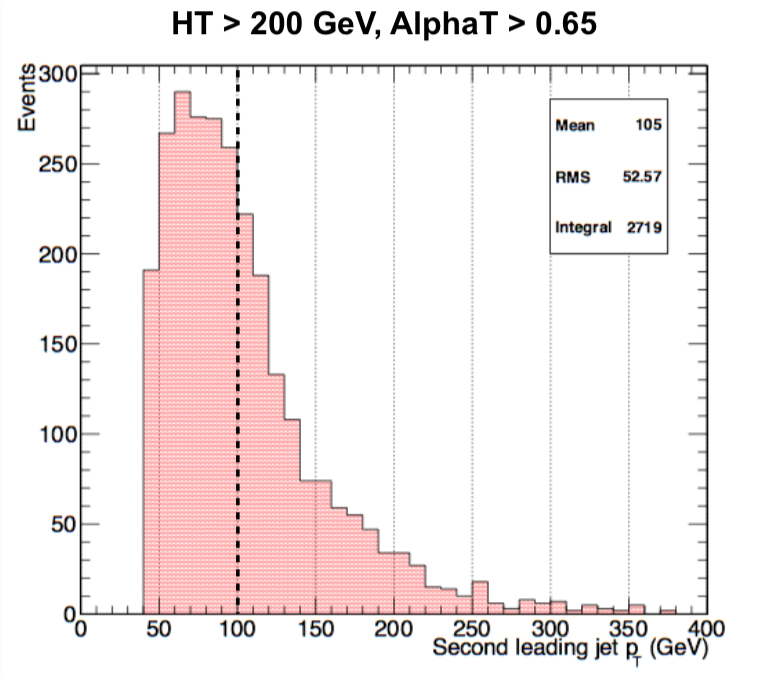
\includegraphics[width=0.5\textwidth]{figures/asymPlots/secondJetPtlowHT}
  }~~
  \subfigure[Second jet \PT for $400\gev<\HT>500\gev$, $\alphat>0.52$]{
    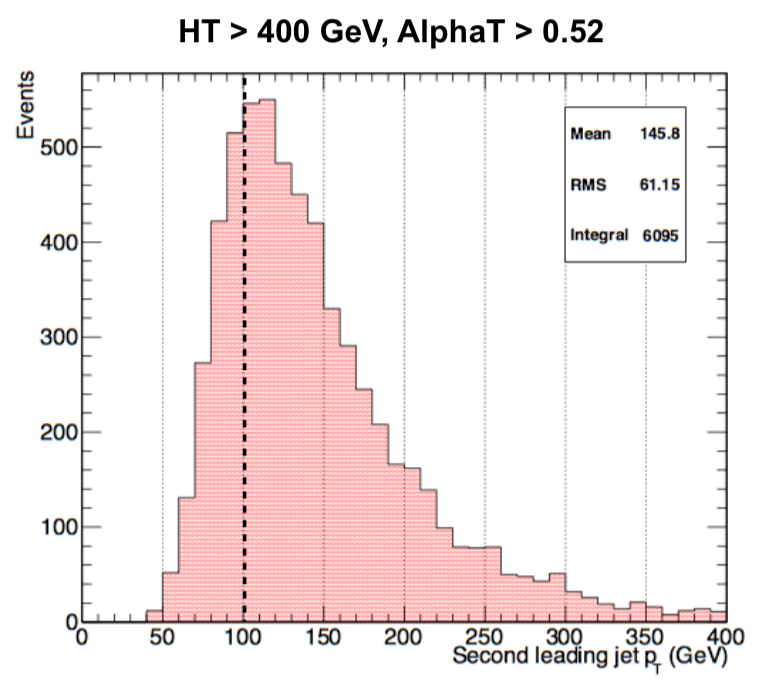
\includegraphics[width=0.5\textwidth]{figures/asymPlots/secondJetPthigherHT}
  }
  \\
  \caption{\label{fig:asymMotivation} The second leading jet \PT for different
  cases of \HT after a baseline signal selection: $\njet\geq2$, lead jet
  $\ET>100\gev$, lepton vetoes. Made with the T2tt ($m_{\rm
    stop}=425\gev$, $m_{\rm LSP}=325\gev$) simplified model sample.}
\end{figure}

